\documentclass{article}

\usepackage[utf8]{inputenc}
\usepackage[T1, T2A]{fontenc}
\usepackage[russian, english]{babel}
\usepackage{tempora}
\usepackage{arxiv}
\usepackage{floatrow}
\usepackage{float}
\usepackage{animate}
\usepackage{caption}
\usepackage{subcaption}
\usepackage{tocloft}



%\usepackage[T1]{fontenc}    % use 8-bit T1 fonts

\usepackage{url}            % simple URL typesetting
\usepackage{booktabs}       % professional-quality tables
\usepackage{amsfonts}       % blackboard math symbols
\usepackage{nicefrac}       % compact symbols for 1/2, etc.
\usepackage{microtype}      % microtypography
\usepackage{lipsum}
\usepackage{graphicx}
\usepackage[super]{nth}
%\usepackage[round,sort,comma,authoryear]{natbib}
%\usepackage{todonotes}
\usepackage[multiple]{footmisc}
\usepackage{csquotes}
%\usepackage[hyperfootnotes=false]{hyperref}       % hyperlinks
\usepackage[hidelinks,linktocpage=true]{hyperref}       % hyperlinks

% customize captions

\DeclareCaptionFormat{custom}
{
    \textit{#1#2}\small{#3}
}
\captionsetup{width=0.9\textwidth,format=custom}

% Change font size of table of content
\renewcommand\cftsecfont{\normalsize}
\renewcommand\cftsecpagefont{\normalsize}
\renewcommand\cftsecafterpnum{\par\addvspace{2pt}}
\renewcommand\cftsubsecafterpnum{\vskip 2pt}

\setlength\cftbeforesecskip{-2pt}
\setlength\cftbeforesubsecskip{-2pt}

\renewcommand{\contentsname}{}
\addto\captionsenglish{\renewcommand{\contentsname}{}}




%\usepackage[nomarkers, nolists]{endfloat}
%\renewcommand{\efloatseparator}{\mbox{}}

%\usepackage[backend=biber,style=authoryear,sorting=nyt]{biblatex} 
\usepackage[backend=biber,style=ieee,sorting=nyt]{biblatex} 
\addbibresource{references.bib}

\selectlanguage{english}

% Make cite be citep so that everything is in parenthesis
%\renewcommand\cite{\citep} 
\renewcommand\cite{\parencite} 

\newcommand{\todo}[1]{} 
%\setuptodonotes{color=black!30, backgroundcolor=white!30}

%add comment
\newcommand{\comment}[1]{}

% Penalize breaking footnotes
\interfootnotelinepenalty=3000

% Set space between footnotes
\setlength{\footnotesep}{12pt}

\graphicspath{ {./} }
%Apophenic
\title{An analogue picture maker}


\author{
  Nisse A.~Bergman \\
  \\
  Spring term 2022\\
  Master essay\\
  Supervisors: Michele Masucci\\
  \\
  Department of Fine Art\\
  Konstfack University of Arts, Crafts and Design\\
  LM Ericssons Väg, 126 26, Hägersten, Sweden \\
  \texttt{nisse.bergman@student.konstfack.se} \\
}

\begin{document}
\maketitle

\begin{abstract}
I present a novel optical device capable of faithfully reproducing
arbitrary images and image sequences by utilizing the interplay between
mirrors and colored surfaces acting as interactive mosaics.\\
My main contribution is describing a method for pre-computing the mirror
lattice configuration and mirror orientation as well as a ways of
finding the corresponding diffuse color pattern in the spatio-temporal
domain. \\
The method is fast enough to allow rapid iteration by enabling
physically based light ray simulation ahead of fabrication.\\
I demonstrate the effectiveness of my method in a wide range of image
and image sequence scenarios as well as multiple device configuration
variants.
\end{abstract}


\section{Introduction}
This master thesis assay is supposed to complement and give a more
thorough understanding of my master exhibition. While this paper is published deep
in the humanities in the fine art department I have opted to write it a
little bit more like one would write an in-depth technical blog or repo
readme\footnote{Open source projects hosted publicly traditionally have
  a file called \texttt{README} that is intended to be read by users or
  contributors of the project before use. The readme file is usually
  placed in the root folder of the repository and commonly contains
  instructions on how to compile and run the project, some code
  examples, code formatting and style rules and sometimes more in-depth
  description of architectural design.} post that might be more familiar
to the \emph{natural scientist} or the casual hobby coder. I will not go
full techno on you but this paper will demand some prior knowledge of
optics and combinatorics to fully comprehend all concepts. That said I
will try to focus on the intuition\footnote{In mathematics the term
  \emph{intuition} refers to a way to reason to a solution of a
  mathematical problem using a broader understanding of a mathematical
  concepts. It doesn't have to be a formal proof but more commonly an
  example. Explaining solutions by first describing the intuition is
  very common in geometry where it is commonly possible to describe
  problems in e.g. lower dimensions.} and add extensive figures and
footnotes where a novice reader of the field can find a primer and an
experienced reader some more depth and details. If you don't feel
comfortable with the nitty gritty as for example the math figures you
can just skip ahead. Since I want this article to work as a traditional
readme-file as well as a science paper I want it to be possible to
reproduce the results by following along in the text. That is why I have
insisted on keeping the mathematical notation and technicalities to retain
utility even though most readers of fine art master theses probably
won't care.

The sculptures I present here are a new kind of device, contraption or
idea that can show images without any (required) moving parts or
electricity. One can say that it is an analogue passive display. It is
using illuminated pixels just as a computer screen\footnote{The most
  common type of computer screens are called Liquid Crystal Display or
  LCD. It works by shining a white back light on a liquid crystal film.
  By applying a polarized electrical current to the LCD-film the film
  can change from opaque to transparent or vice versa. By having red,
  green and blue filters the transmitted light can be either red, green
  or blue. Combining red, green and blue light with different
  intensities one can make the human eye perceive a large portion of the visible spectrum. One unit of red,
  green and blue is called a pixel. By putting a huge number of pixels
  together in a grid one can make electronic mosaics and produce any
  picture or animation.} does, but in my case the pixels are not small
lamps but mirrors. Each mirror works just as a pixel or a mosaic tile
contributing with one small piece of the overall image. By orienting
each mirror so that they reflect a color from somewhere else in the
room it is possible to make the mirror appear to have a color. Hence,
by painting a surface in a room it is possible to make sure that any
desired color are available to be reflected. After realizing that it is
possible to reflect a predetermined color from a predetermined position
in the room one can experiment with endless possibilities of arranging
the colors to be reflected. I have focused on four different variants
that I will talk about in this paper that I have also built physical
models of. The first one consists of a disc with painted eccentric
color fields. This variant makes it possible to create animations by
having the disc rotate around its minor axis thereby alternating what
colors is at the reflection focal points. The second variant is a
cylinder that rotates around its vertical axis and also enables an
animation. Then I'm showing the most basic variant which consists of a
rectilinear array of color fields that in my case only creates one
image per mirror setup but can be used to show multiple images using
multiple mirror setups while reusing the color fields.

I have structured this paper to discuss all the elements of making an
image with mirrors and color fields including:

\tableofcontents


\clearpage

\section{A brief history and background}
Fine art has a long history of making pictures that exploit how the
human vision merges small dots in close proximity into perceiving it as
one coherent shape. One example is ceramic, glass or stone mosaics with
examples as old as the 3\textsuperscript{rd} millennia BCE in
Mesopotamia. Mosaic patterns with pictures became widespread during the
classical era both in Ancient Greece and Ancient Rome. This is maybe the
first example of using small colored dots that blend in the human
perception into a picture.

In the late 1800s a painting technique called \emph{Pointillism} emerged
with prolific practitioners like Georges Seurat\footnote{Georges Seurat,
  1884--1886, \emph{A Sunday Afternoon on the Island of La Grande
  Jatte}, oil on canvas, 207.6 × 308 cm, Art Institute of Chicago} ,
Vincent can Gogh\footnote{Vincent van Gogh, 1887, \emph{Self Portrait},
  oil on canvas, 41 × 32.5 cm, Art institute of Chicago} and Paul Signac
\footnote{Paul Signac, 1901, \emph{L'Hirondelle Steamer on the Seine},
  oil on canvas, National Gallery in Prague} and a bit later for example
Robert Delauney\footnote{Robert Delaunay, 1906, \emph{Jean Metzinger},
  oil on paper, 54.9 × 43.2 cm, Museum of Fine Arts, Houston}.
Pointillism heavily relies on the fact that small dots of paint close
together is merged in the human brain into a single surface. Instead of
using a lot of color shades some shades can be made by mixing dark and
light dots with different densities. This phenomena is exploited in many
related but distinct techniques in different media. In printmaking the
technique is adapted to paper and called \emph{half toning} where dots
of, usually, cyan, magenta, yellow and black ink are printed in a raster
with different sizes. In computer science where it is usually restricted
to rectilinear arrays it is called \emph{dithering} and typically includes
a restricted color palette. In engraving there is a technique called
\emph{stippling} that similar to pointillism but only one color is
used. All techniques are basically the same with some modifications for
each medium.

When artists got access to the early computers in the 50s the output was
usually limited to oscilloscopes. Herbert W. Franke published some of the earlier
computer generated works in \emph{Kunst und Konstruktion} already in 1957 \footnote{Herbert W. Franke, 1957, \emph{Kunst und Konstruktion}}
that contains multiple examples of this.

Later in the 60s when computers got the ability to print paper strips with a fixed-width
font (e.g typewriter typefaces like Courier) artists started using that technology too.
Computer art pioneers like Kenneth Knowlton and Leon Harmon\footnote{Ken Knowlton, Leon Harmon,
  1967, \emph{Computer Nude (Studies in Perception I)}, 86.36 x 182.88
  cm, silkscreen print} used those limitations and made shaded pictures
with only text by treating the different characters as different gray
scale pixels. This has later become known as ASCII-art\footnote{The name
  ASCII comes from the 1963 character encoding called \emph{American
  Standard Code for Information Interchange} specifying what characters
  that can be used}. In the mid 70's to early 80's this was one of the
most common computer game graphics modes. With the release of 8-bit (256
color) video game console \emph{Nintendo Entertainment System} in the
early 1980s the \emph{8-bit pixel art} was popularized and featured lots
of perceptual tricks using the limits of what pictures can be made with
a very limited palette.

Using mirrors and optics to create a picture is also not a new idea. The
Stanford physics PhD Ben Bartlett\footnote{Ben Bartlett, 2021,
  \emph{3d-printed-mirror\_array},
  \url{https://github.com/bencbartlett/3D-printed-mirror-array}} used a
similar and independently invented idea as mine. He published, just a month ago at the time of writing, a
project that created a "Will you marry me" message to his future partner on a beach
with a hand held 3d-printed array of small mirrors. Interestingly for
this paper he has also published a technical readme-writeup in his
GitHub-repo. From academia we have for example got the interesting paper
called \emph{High-contrast Computational Caustic Design}\footnote{Yuliy
  Schwartzburg, Romain Testuz, Andrea Tagliasacchi Mark Pauly, 2014,
  \emph{High-contrast Computational Caustic Design}} that was published
in 2014 describing how a flat transparent surface can be shaped so that
the caustics\footnote{When for example the sun rays hit the water of a
  pool they refract penetrating the waves and fills the bottom of the
  pool non-uniformally with areas of high light intensity and others
  with low. This phenomena is called caustics.} produce an arbitrary
picture. Using the same technique the less academic but
still-aerospace-engineer Matt Ferraro published a technical
writeup\footnote{Matt Ferraro, 2021, \emph{Hiding Images in Plain Sight:
  The Physics Of Magic Windows} ,
  \url{https://mattferraro.dev/posts/caustics-engineering}} with
sourcecode in 2021 where he explains how to make your own with a
CNC-router while leaning heavily on a previous paper from 2014 by Yue et
al. \footnote{Yonghao Yue, Kei Iwasaki, Bing-Yu Chen, Yoshinori Dobashi
  and Tomoyuki Nishita, 2014, \emph{Poisson-Based Continuous Surface
  Generation for Goal-Based Caustics}}. When researching this paper I
found that Swedish artist Christian Partos \footnote{Christian Partos,
  2003, \emph{MOM (Multi Oriented Mirrors)},
  \url{http://www.partos.se/Www/SidorE/MOM.htm}} used a similar idea as
mine but instead of color-fields he used the falloff from a spotlight
as the palette. I would also like to mention Daniel Rozin\footnote{Daniel
  Rozin, 2011, \emph{Brushed metal mirror},
  \url{http://www.smoothware.com/danny/brushedmetalmirror.html}} who has
made multiple sculptures involving mirrors (although computer
controlled).

\section{Picking a suitable image or images for
reproduction}

As will become apparent in just a few moments it is a lot easier to
reproduce an image that contains few unique colors than one that
contains all possible shades. This is usually referred to a
\emph{reduced palette} in contrast to use all possible colors. The
obvious drawback of using a reduced palettes is that the fidelity of the
image will also be reduced if the originals palette does not match the
reduced. Fortunately computer games had to work with these
limitations\footnote{For example the very popular \emph{Nintendo
  Entertainment System} (1984) could display a total of 25 different
  colors at a time. The original \emph{Game Boy} (1989) could only
  display four shades of green. The \emph{Sega Master System} (1985)
  could display 64 colors but only 31 on screen at the same time while
  the \emph{Mega Drive} (1988) increased that to 512 colors and 61
  simultaneously on screen.} for many years during the 70's, 80's and
early 90's with the effect that a lot of research was put in to find clever ways to
hide the artifacts that appears when using a reduced palette.

In general there are two kinds of images that works well with a reduced
palette. Either very noisy images with a lot of high-frequency details
\footnote{High frequency details are large changes in colors over a
  small distance. The classic example is pictures of stormy water. Low
  frequency details are the opposite. Putting a blur filter on low
  frequency details doesn't change much.}or solid color fields as for
example cartoons. The in-between with smooth gradients are trickier. The
reason noisy images works well is that when you reduce the color
palette the result will also be noisy and the image will be perceived as
noisy both before and after. Low frequency details like shades and
gradients tend to produce aliasing artifacts that is more difficult to
hide with few colors. Cartoon style images doesn't contain shades or
gradients and are produced with the constraint of a reduced palette in
mind.

The image one wants to create generally is going to be low resolution
given the fact that one will have to fabricate it later and an image
with two million mirrors will be quite a project. One can also bear in
mind each mirror will be very large in comparison to for example a
computer screen pixel. It can be smart to take inspiration from digital
images that are made to work being very small. The obvious example that
comes to mind is application icons that are meant to be legible even at
very small sizes. Another inspiration can be emojis or emoticons that
are created to flow in text\footnote{An iPhone 13 has about 4.7 million
  pixels. With a density of 460 pixels per inch and a size of 146x71 mm
  it makes it to about 80.000 pixels per square centimeter. An emoji set
  with the standard font size is about 3x3 mm meaning it contains about
  25.000 pixels.} while being legible at those small sizes.

If the image should contain multiple frames like an animation or a
slideshow one also has to think about the sum of colors in all images.
In that case it can be beneficial to pick images that contain the same
colors to not expand the palette too much. We will come back to that
later.

\section{Selecting an optimized color palette, or \emph{color quantisation}}

We have established that we want to produce images with a reduced
palette. The easiest way is of course to draw the images with a reduced
palette to begin with and we don't have to reduce the palette but say we
don't have that option.

Say we have an arbitrary image and want to use an already existing
palette. Maybe we for example only have a certain number of paints that
we cannot mix. The naïve approach to solve this issue is to iterate over
all pixels and then compare their colors to all colors in a predefined
palette finding the one most similar. Sometimes, if we are lucky, and
depending on the palette and image, the difference may not be easily
detectable with the human eye. A shades of red in the image might be
just a hair different from the paint we have at hand but so using that
might not make any noticeable difference\footnote{Noticeable is of
  course a relative term related to perception which makes any error
  hard to qualify. This paper is long enough as it is.}. At a first
glance this seems like a reasonable approach but when digging a bit
deeper it will become apparent that just defining what "closest"
actually mean is very hard. What happens when the image contains
hundreds of shades of red and the palette only one? What happens if it contains none?

An other scenario is that one don't have a predefined palette. Say you
can mix any paint color but you can only use five. Then you want to
somehow compute the palette that has the maximum perceived similarity to
the original and this problem is incredibly hard. In the technical literature this
problem of having a palette with a lot of colors and reducing it to a
palette with few colors is referred to as \emph{color space
quantisation}\footnote{In mathematics and signal processing
  \emph{quantisation} is the process of mapping a large often continuous
  set into a smaller countable set often with finite elements.}.

This problem is computationally very hard for exact solutions (if any
exist) but there are algorithms that can produce good approximations.
The standard color space quantisation algorithm that is used in for
example Photoshop is called \emph{k-means clustering}\footnote{K-means
  clustering (or sometimes the \emph{Lloyd--Forgy algorithm} ) formally
  aims to partition \emph{n} observations into \emph{k} clusters in with
  each observation belongs to the cluster with the nearest mean.}\footnote{Edward W. Forgy, 1965, \emph{Cluster analysis of multivariate data: efficiency versus interpretability of classifications}.} and
was invented in 1957. It basically finds \(n\) points in s spectrum so
that the distance from all colors locations is minimized. Another
common algorithm is \emph{Median Cut} that is used less these days
because of its poor quality. K-means and Median Cut tends to produce
washed out colors when reducing the palette to very few colors. 
This is due to the fact that if one mixes opposite colors the result is gray
and since k-means clustering by definition is trying to find the mean 
color the result will tend to be gray. Two different, slightly
better, but slow and resource intensive algorithms is \emph{Hierarchical
Agglomerative clustering} and \emph{Spatial Color Quantisation} that
were both published in 1994. Another algorithm that I have tested is the
\emph{NeuQuant} algorithm by Anthony Dekker\footnote{Anthony H. Dekker,
  1994, \emph{Kohonen neural networks for optimal color quantization}},
also from 1994, that uses pretrained Kohonen neural networks to find the
best palette and assign each pixel one color from it. It tends to
favor the smoothness of larger gradients over the retention of visually
distinct, but less frequent hues. Also, can introduce edge artifacts
when used with graphics since it's not designed for working with a small
number of colors. I have settled for \emph{RgbQuant}\footnote{Leon Sorokin, 2015, https://github.com/leeoniya/RgbQuant.js} by Leon Sorokin that is
specifically made for small palette graphics and also has the benefit of
being published in 2013 and hence can use a lot of the findings of
previous research.

If we want to create an animation with multiple images the size of the
problem scales up linearly with the number of frames. Instead of each
mirror only showing one color each mirror should be able to show a
sequence of colors so when the palette is reduced the entire sequence
needs to be considered.

\begin{figure}[ht!]
\centering

    \begin{subfigure}{0.5\textwidth}
         \centering
         
\includegraphics[scale=1.0]{images/walkthrough/start.png}
     \end{subfigure}
     
     \begin{subfigure}{0.5\textwidth}
         \centering
         
\includegraphics[scale=1.0]{images/walkthrough/palette.png}
     \end{subfigure}

\caption{An example image of a hamburger containing thousands of colors (top) and the automatically computed palette reduced to only nine colors using the RgbQuant-algorithm (bottom)}
\end{figure}





\section{Ways of refining the reduced palette to create perceived gradients and shades}

Now we have an optimal palette. How do we assign the palette colors to each mirror?
As we saw in the History section there are many examples of artists
emulating gradient and shades with few colors (e.g. dithering,
stippling, half toning). For our purposes dithering is the best approach
since it is used on a grid with the points having the same distance and
same size. Dithering works by intentionally apply a carefully crafted
noise to the image that prevents large scale patterns as color banding.

\begin{figure}[ht!]
\centering

\includegraphics{images/walkthrough/threshold.png}
\caption{The hamburger example from above using the same example palette. Here is the baseline result when just 'snapping' each pixels color to the color most similar in the palette. This is technically called the nearest-neighbor algorithm. It is possible to see the banding effect in the red on the bun.}
\end{figure}

There are a lot of different dithering algorithms but they roughly fall
into three different categories namely \emph{random dithering}, \emph{ordered dithering} and
\emph{error diffusion dithering}. In the \emph{random dithering} category we simply have
algorithms that add a random noise with a bias to the underlying color
to break up the banding. This tend to have the effect that larger smooth gradients are handled well but smaller details usually disappears in the noise.

\begin{figure}[ht!]
\centering
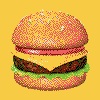
\includegraphics{images/walkthrough/noise.png}
\caption{Random noise dithering.}
\end{figure}

In the ordered category we have \emph{half-tone-},
\emph{void-and-cluster-} and \emph{Bayer matrix-dithering}. They
generally create a distinct patterns that was very common in the early
Super Nintendo era.

\begin{figure}[ht!]
\centering
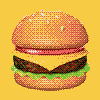
\includegraphics{images/walkthrough/bayer.png}
\caption{Bayer matrix dithering.}
\end{figure}

The more interesting methods are the error-diffusion dithering
algorithms that tries to, as the name suggests, diffuse the error of the
difference between actual color and the available palette color over
its neighbouring pixels. The most common of the error-diffusion
dithering algorithms and also the oldest are
\emph{Floyd-Steinberg}\footnote{Robert W. Floyd and Louis Steinberg,
  1976, \emph{An adaptive algorithm for spatial grey scale - Proceedings
  of the Society of Information Display 17}} from 1976. A modified
version of this is still considered state of the art and is used in for example Photoshop. 
Independently and almost at the same time Jarvis, Judice and Ninke of Bell Labs
developed a similar algorithm\footnote{J F Jarvis, C N Judice, and W H
  Ninke, 1976, \emph{A survey of techniques for the display of
  continuous tone pictures on bilevel displays. Computer Graphics and
  Image Processing}} that takes more neighboring pixels into account. To improve on the resulting quality and/or
computation speed a number of spinoffs and variants that diffuse the
error slightly differently were developed by Peter Stucki in 1981, Bill
Atkinson\footnote{Bill Atkinson also invented the double click while
  working at Apple Computers} in the mid 1980's, Daniel Burkes in 1988
and Frankie Sierra in 1989. They all produce slightly different results
and have different pros and cons. In some of the examples below one can
see that the quantisation-error has diffused out into the solid
background. The way to pick one is basically a matter of taste and the
type of image used.

\begin{figure}[ht!]
\centering
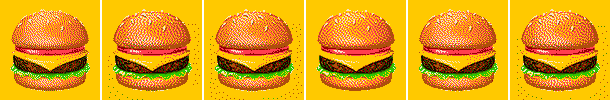
\includegraphics[width=0.9\textwidth]{images/walkthrough/all-dithering.png}
\caption{Diffusion dithering algorithms. From the left Floyd-Steinberg, Jarvis-Judice-Ninke, Stucki, Atkinson, Burkes and Sierra. The main differences can be seen in the cheese and the background.}
\end{figure}


\section{Considerations of how to arrange the mirrors}

We want the image made by the mirrors to look vibrant hence we need to reflect
as much light as possible. We do that by covering as much of the substrate that
the mirrors are attached to. All the area not covered by a mirror will
have its own color and that color affects the overall picture,
basically mixing with the colors of the image, so we want to reduce that area as
much as possible. To do that we need to find a shape of mirrors and a
pattern of tiling that covers the most amount of area and exposes as
little as possible of the background surface.

We also need to think about what is reasonable in terms of effort. It is
only easy to find square and round circles off the shelf. We will need
thousands of mirrors and having to fabricate odd shaped ones is not
really a viable option.

Square mirrors seems to be the obvious choice but for reasons we will
discuss later we want to use round mirrors since they have some good
properties when we come to fabricating. While square tiling of square
tiles are 100\% efficient round mirrors arranged in a rectilinear are
not and will leave a lot of gaps in-between them. We can do better and
fortunately people have been studying this thoroughly and proved that
most dense packing of circles on a plane is, not surprisingly, the hexagonal array packing.

\begin{figure}[ht!]
\centering
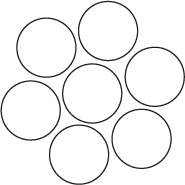
\includegraphics{images/circular-pattern.png}
\caption{Hexagonal packing}
\end{figure}


This is the same honeycomb packing bees use in their beehives
\footnote{The density of packing circles on a plane with diameter \(D\)
  is
  \(\frac{3\pi}{4}D^2 \big/ \frac{3\sqrt{3}}{2}D^2= \frac{\pi\sqrt{3}}{6} \approx 0.9069\)
  i.e. about 10\% of the light will be hitting the substrate instead of
  a mirror. Variant of this problem have been solved by scientific
  superstars for example Kepler, Lagrange and Gauss.}. It is
proven\footnote{Hai-Chau Chang and Lih-Chung Wang, 2010. \emph{A Simple
  Proof of Thue's Theorem on Circle Packing}}\footnote{Proven by Joseph
  Louis Lagrange in 1773} to minimize the space between the round
mirrors and hence reflect more light per unit area and therefore allow
for a more vivid image.

Using a hexagonal grid does have the drawback that since out original
digital image that we want to make a mirror-image of will most definitely
be a rectilinear grid we will have to convert the coordinates to
hexagonal. This can be done in multiple ways \footnote{A great source of
  information on hexagonal grids can be found here
  \url{https://www.redblobgames.com/grids/hexagons/}}. Just mapping
from a rectilinear to a hex grid will make the image shrink on one of
its axes (depending on the hex arrangement). This is due to the fact that 
the hexagonal shape has three symmetric diagonals that are longer than the sides.
One can implement some kind of sub pixel sampling like a \emph{bicubic interpolation}\footnote{See
  for example Dianyuan Han, 2013, Comparison of Commonly Used Image
  Interpolation Methods}or just account for the difference by
pre-scaling the magnified axis by \(\frac{3}{2}\) To compensate.

Of course, the objective might not be to optimize for area coverage but
some other aesthetic quality but that is beyond the scope of this paper.

\section{A very brief primer on light transport}

To be able to follow along in the coming sections we need to explain
some basic concepts of light transport. Feel free to skip this section
if you feel comfortable with basic optics.

Light rays travel in a straight line through a medium (like air). When
striking a surface some of the light will be absorbed by the surface
(converted to heat) and some will bounce back, reflected. The absorption
is what makes object look colored due to that the surface absorbing
some frequencies of light more than others. On a perfectly flat, smooth
surface, called a specular surface, the angle of incidence, the angle at
which the light ray hits the surface, is equal to the angle of
reflection with regards to a projected line perpendicular to the
surface, known as the normal.

\begin{figure}[ht!]
\centering
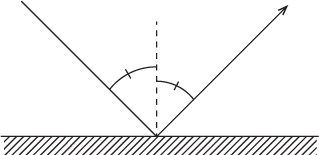
\includegraphics{images/reflection.png}
\caption{Angle of incident and angle of reflections equal with regards to normal (dashed)}
\end{figure}


On rough surfaces, called diffuse surfaces, the light will reflect in
slightly different angles all over the surface but still retaining its
energy. A mirror is said to be more specular than a painted wall that is
said to be diffuse.

\begin{figure}[ht!]
\centering
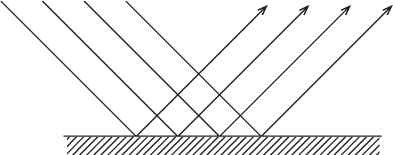
\includegraphics{images/specular-reflection.png}
\caption{Specular reflection}
\end{figure}


\begin{figure}[ht!]
\centering
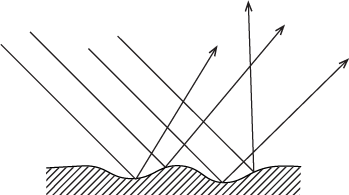
\includegraphics{images/diffuse-reflection.png}
\caption{Diffuse reflection}
\end{figure}


For opaque materials all the light will either have to be reflected or
absorbed. If the material is transparent or translucent some of the
light might pass into the material. When passing into a material the
light ray bends from its angle of incidence. This phenomenon is called
refraction. The amount of bending is due to the relative indices of
refraction (also called the optical density) of the medium the ray
travels from and the medium the ray travels into (described by
\emph{Snell's Law}). The larger the difference between the media the
more the ray bends\footnote{To be specific the refractive index varies
  slightly with the wavelength of light. Generally the refractive index
  decreases with increasing wavelength. This leads to an effect called
  \emph{Chromatic aberration} that for example in lenses manifests
  itself as fringes where the light is split into its constituent
  frequencies with slightly different focal points. There is also
  something called \emph{Critical angle} which is the angle at where
  light is not refracted but instead reflected. If the angle of
  incidence is greater than the critical angle all light will be
  reflected. This is the phenomena that makes fiber cables work by
  bouncing the light inside a transparent glass fiber, called
  \emph{total internal reflection}. This is also the phenomena, called
  the \emph{Fresnel effect}, that makes a calm lake at sunset appear as
  a mirror although being a poor reflector at normal incidence. For
  reference air has a refractive index very close to 1.00 while the
  value for window glass is about 1.52.}.

\begin{figure}[ht!]
\centering
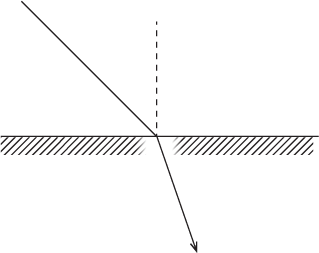
\includegraphics{images/refraction.png}
\caption{Refraction}
\end{figure}

For our purposes we can largely disregard both refraction and
diffuseness. We also don't have to consider translucency, internal
reflections, subsurface scattering, Fresnel effects, chromatic
aberration or any other obscure phenomena present in the real world
since it will not make any noticeable difference that we can adjust for
anyway. We will consider the mirrors we use to be ideal mirrors that are
perfectly flat, covered with a perfectly transparent glass with the same
refractive index as the surrounding media and the reflective surface to
be perfectly specular \footnote{In theory it would be possible to use
  \emph{first surface mirrors} in which the reflective surface is the
  front instead of on the back of the glass. First surface mirrors are
  commonly used in high precision optical equipment such as cameras,
  telescopes and lasers but are also considerably more expensive
  starting at around 400 times the price of a regular second surface
  mirror.}. For us the only thing that matters is that incident and
reflected light rays have the same angle in respect to the average
surface normal.


\section{How to compute the orientation of each individual
mirror}

We cannot (or at least we don't want to) take all physical phenomena
into consideration when doing these calculation since that would be
extremely tedious and wouldn't improve the result noticeable therefore
we are going to simplify. We are going to do all computations using an idealized
mirror reflects all light striking it, without absorbing any light, it
itself doesn't have any inherent color. It appears as it has the color
or colors of whatever it reflects, of course also depending on your
vantage point. If we for example paint a wall blue, and stand with our
back against it with a mirror in front of us, the mirror will look as
blue as the wall. If we paint the wall with a color spectrum and adjust
either the angle of the mirror or our own position we can make it
reflect any point on that surface we want and thereby taking the color
of it. If we want the mirror to look red we can adjust the angle in such
a way that it will reflect a red point. If we want it green we adjust it
accordingly. This is something we can use to decide what color the
mirror should appear as.

\begin{figure}[ht!]
\centering
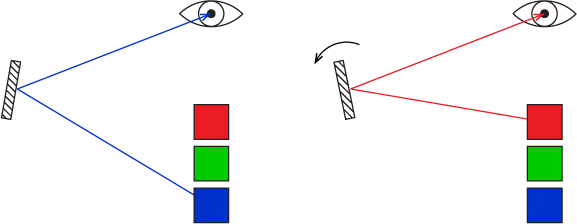
\includegraphics{images/change-color.png}
\caption{The same mirror can appear to be one of multiple colors by rotating the mirror. In the left picture the mirror will appear blue while in the right it will appear red.}
\end{figure}


To calculate what angle the mirror has to have to reflect the light from
a point on the wall, to our eye, is fairly trivial. We
know that the face of the mirror needs to point in such a way that the
angle of incidence and the angle of reflection should be equal in
regards to the mirrors surface normal. The position of the mirror, the
angle of incidence and reflection is known so that leaves us to solve for 
the optimal mirror surface normal. Suppose we have a color field with
the center \(t\). We also have the position of the spectators eye \(e\)
and the center of the mirror \(m\). This gives us equation 1:
\(\vec{i}=e-m, \vec{r}=t-m\)\\
where \(\vec{i}\) denotes the vector of incidence and \(\vec{r}\) the
vector of reflectance. The mirrors normal \(\hat{m}\) is bisecting the
normalized\footnote{A normalized unit vector is denoted with a hat, e.g.
  \(\hat{r}=\frac{\vec{r}}{\|\vec{r}\|}\) where the magnitude of a
  vector is denoted with double bars. The magnitude can be computed, in
  3d euclidian space, with \emph{Pythagoras theorem}:
  \(\|\vec{r}\| = \sqrt{r_x^2 + r_y^2 + r_z^2}\)} vectors of incidence
and reflectance: \(\hat{m}=\frac{\hat{i}^{-1}+\hat{r}}{2}\)\\
Bisecting the angle can be done by adding the two vectors and then
splitting the sum in half making it a unit vector (called the \emph{half
vector}).\\
By aligning the mirrors normal with the half vector we get a perfect
reflection of the color field in the mirror with respect to the
spectators position.

\begin{figure}[ht!]
\centering
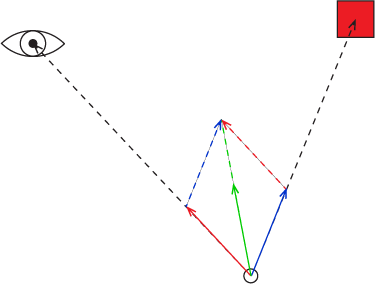
\includegraphics{images/finding-normal.png}
\caption{A visual representation of Equation 2. finding the normal (green). The blue represents the inverted vector of incidence and red the reflected. Adding blue and red and then scaling the sum by 0.5 gives green. From the eye´s point of view the mirror will appear red.}
\end{figure}


So this gives us the basic tools to "set the color" of our mirrors. In
the figures above this has been shown to work in two dimensions (for
clarity) but the math generalizes to three dimensions.

We can now create a "color palette" that we then can "sample" colors
from by adjusting the angle of our mirror. If this mirror is fairly
small it can essentially work as a single pixel that can take any color
from the palette and reflect that into the spectators eye.

So far we have thought of the light as a single ray that strikes a point
of the palette, a point of the mirror and the a point of the spectators
eye but that is a too big of a simplification. If we think of the rays
from the eye (so in reverse\footnote{Although the light rays starts at a
  light source, bounces and scatters off the colored surfaces, reflects
  in the mirrors and strikes the spectators retina it is sometimes
  easier to think of the process in reverse. We don't care about any
  photon that does not hit our eye and the math will add up the same in
  both directions\footnotemark{}. This is actually a very common
  technique in 3D graphics raytracing.}) that strike the mirror they
will form a cone with the apex in the eye and the base covering the
mirrors surface. It is only the rays within that cone that we will be
concerned with. This cone is usually called a \emph{frustum}\footnote{Technically
  a frustum is a geometric shape that has two parallel planes but here
  we use it slightly looser as in the term \emph{viewing frustum} that is generally used
  in the computer graphics literature.} and represents the region
visible in the mirror reflection. When the rays reflect in the mirrors
the frustum will continue extending with the same taper until it strikes
the color fields. The surface area that will be covered by the frustum
on the color fields is related to the surface area of the mirrors and
the combined distances between the eye, mirror and color surfaces.

Doubling that distance will quadruple the area (due to the \emph{The
inverse square law}). This is important since having too small color
fields in relation to the distance from the mirrors will make the mirror
pick up a larger area than one color field and since it's a square law
and not linear small changes in distance makes for bigger changes in
area.

\begin{figure}[ht!]
\centering
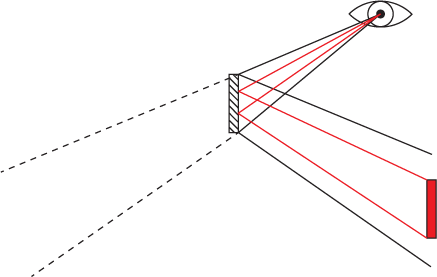
\includegraphics{images/inverse-square-law-frustum.png}
\caption{The frustum extends from the eye subtending the mirror (stroked) and is reflected. The reflected part of the frustum is then larger than the color field (red) picking up the color of whatever surrounds it.}
\end{figure}


This leads to another phenomena that we have to at least consider: One
could assume that the shape reflected in a circular mirror would also be
a circle but that is not always the case. If the frustum from the mirror
and the color fields does not strike the color fields completely
perpendicular the frustum will be "cut off" at a slanted angle, in
geometry the shape formed by the intersection is called \emph{a conic
section} and is is elliptical and not a circle\footnote{The conic
  section is actually one of the mathematical definitions of an ellipse.}.
An example of this is when you are out walking a dark night and shine
your torch light on the ground. If you shine it straight down you would
see a circular light beam but if you shine it further ahead of you it
forms an ellipse. The further away from you the more elliptical and
larger the lights shape will be.

\begin{figure}[ht!]
\centering
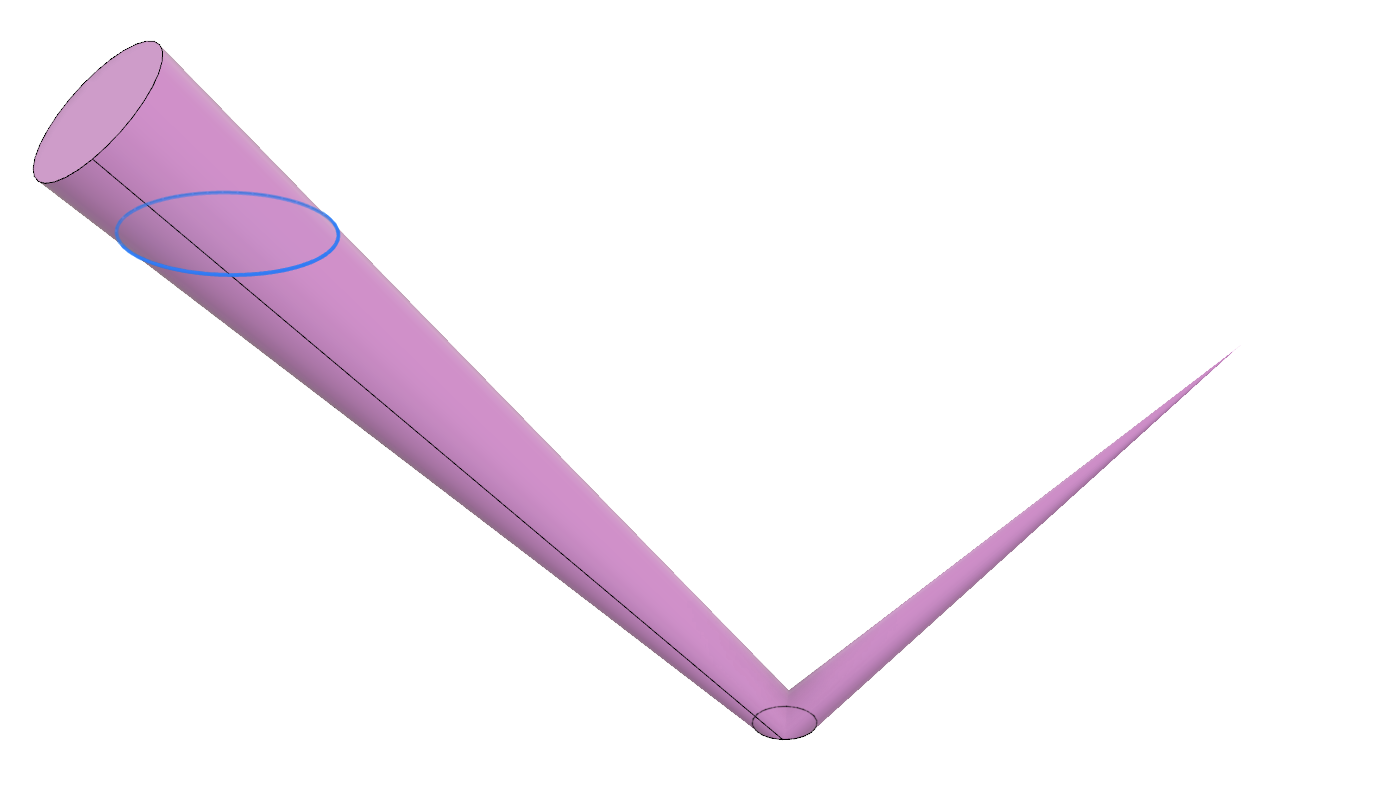
\includegraphics[width=\textwidth]{images/conic-section-1.png}
\caption{Here a light beam (magenta) is reflected in a circular mirror (bottom) at 45° and strikes an imagined parallel wall. The resulting conic section (blue) is elliptical.}
\label{fig:conic_section}
\end{figure}


\begin{figure}[ht!]
\centering
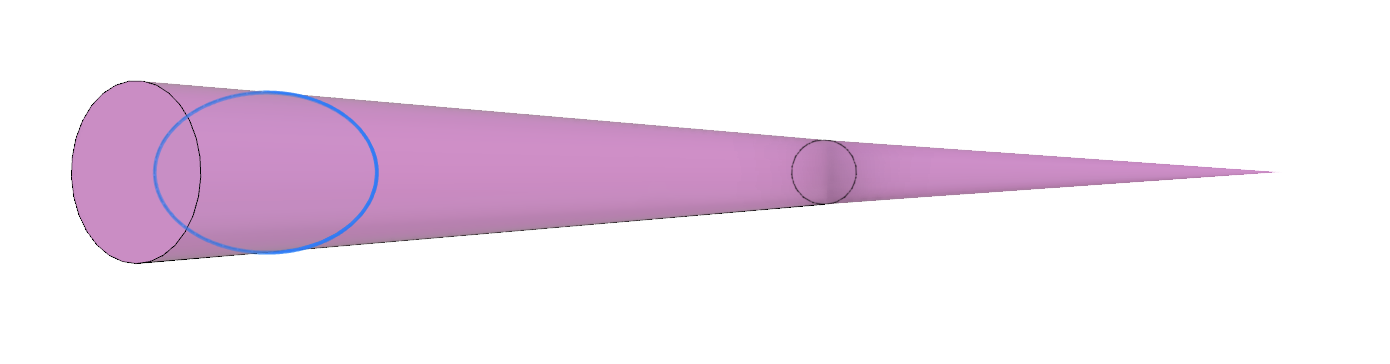
\includegraphics[width=\textwidth]{images/conic-section-2.png}
\caption{The same scene as figure \ref{fig:conic_section} but viewing straight down at the mirror (the rightmost black circle). The elliptical conic section is apparent (blue).}
\end{figure}


This means that the reflected surface of the color field will not
generally be a perfect circle but an ellipse. Depending on where on the
color fields the mirrors are reflecting the shape of the reflecting
area will be differently shaped and sized.

The more extreme the angle of incidence of the cone the more extreme the
proportions of the ellipse will be. As the angle of incidence approaches
tangency to the surface the length of ellipses major axis will approach
infinity. We need to make sure that the entire area inside the
silhouette of the reflected shape will be cover only the color we want
it to cover and nothing else.

What I want to stress with this section is that we cannot simply think
of the sampling of the palette as a point sampling but an area sampling
and to be more specific an elliptical area. This shape and area changes
depending on the angle of the rays between the mirror and the palette.

Since we now know that the mirror will sample colors from an area it
might be a good idea to paint the colors of the palette as fields so
that the entire sampled area is the same color. Making the palette
color fields slightly oversized allows for some errors (in e.g mirror
angle and positions) while still fitting the frustums base inside it.

One way we could do is to line up all the colors in the palette in a
vertical column and have the mirrors point to whatever color it needs to
reflect. In the example below (fig. \ref{fig:one_image_3d}) we can see how the rays reflects on the
mirrors that are rotated in such a way that the light strikes one of the
five color fields. The effect can only be seen when viewing the mirrors
from the precalculated position.

In the example below we need one color field per color in the image.
All mirrors assigned to yellow points at the same area inside the yellow
field. All that are assigned blue point to a point inside the blue etc.

\begin{figure}[ht!]
\centering
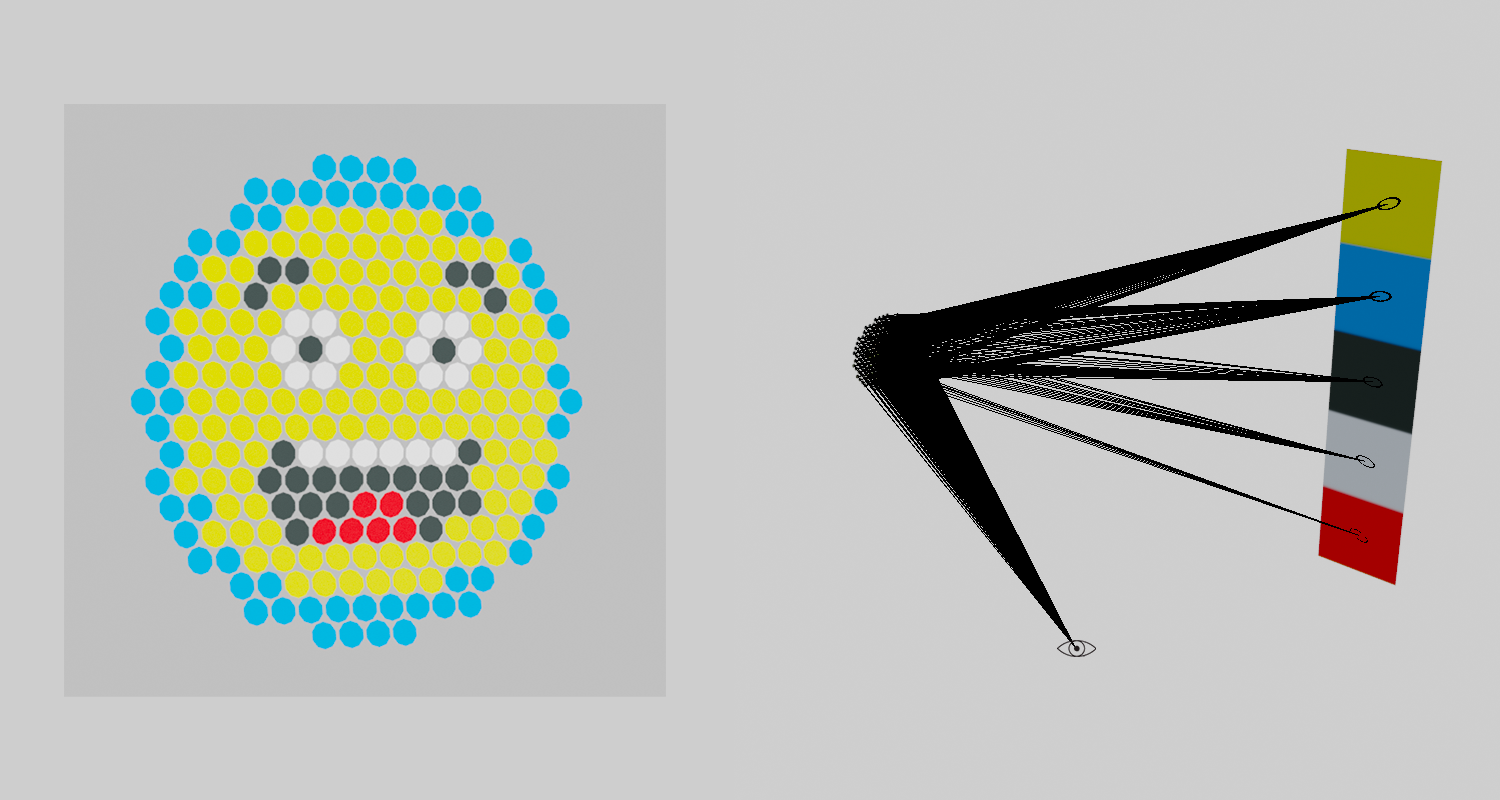
\includegraphics[width=\textwidth]{images/one-image-3d.png}
\caption{A computer generated rendition of the mirrors appearing to be colored when seen from the correct location (left). The light rays bouncing on the mirrors and a color palette with five colors (right). Note the ellipses on the palette that represents the light stricken area and the rays only represents the single ray that hits the center point of that area.}
\label{fig:one_image_3d}
\end{figure}




If we replace the palette with another palette that has different
colors the image will of course change. If we are careful with what
colors the first and second palette has we can actually make two valid
images without touching any mirrors. To do this we need to think of each
mirror being assigned a sequence of colors instead of just a single
color.

If we place two vertical lines of colors we can think of one column as
a frame of an animation and the rows as the sequences of colors
assigned to mirrors. To change frame we can simply shift the palette
left and right so that the mirrors reflections either strike the left or
the right column (fig. \ref{fig:two_image_3d_frame1}-\ref{fig:two_image_3d_frame2}).


\begin{figure}[ht!]
\centering
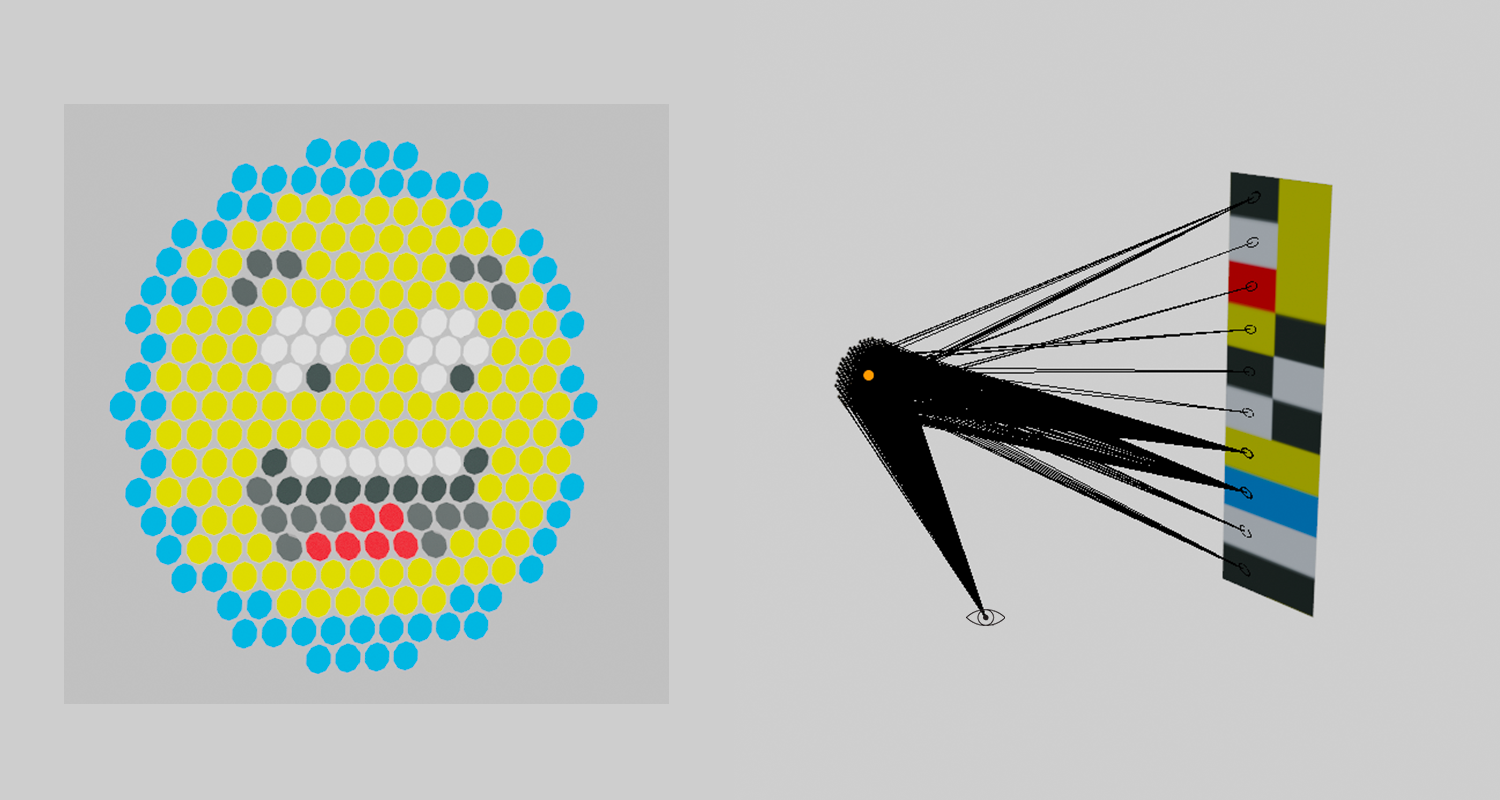
\includegraphics[width=\textwidth]{images/two-image-3d-frame1.png}
\caption{When the mirror points to the left column of color fields in produces one image.}
\label{fig:two_image_3d_frame1}
\end{figure}

\begin{figure}[ht!]
\centering
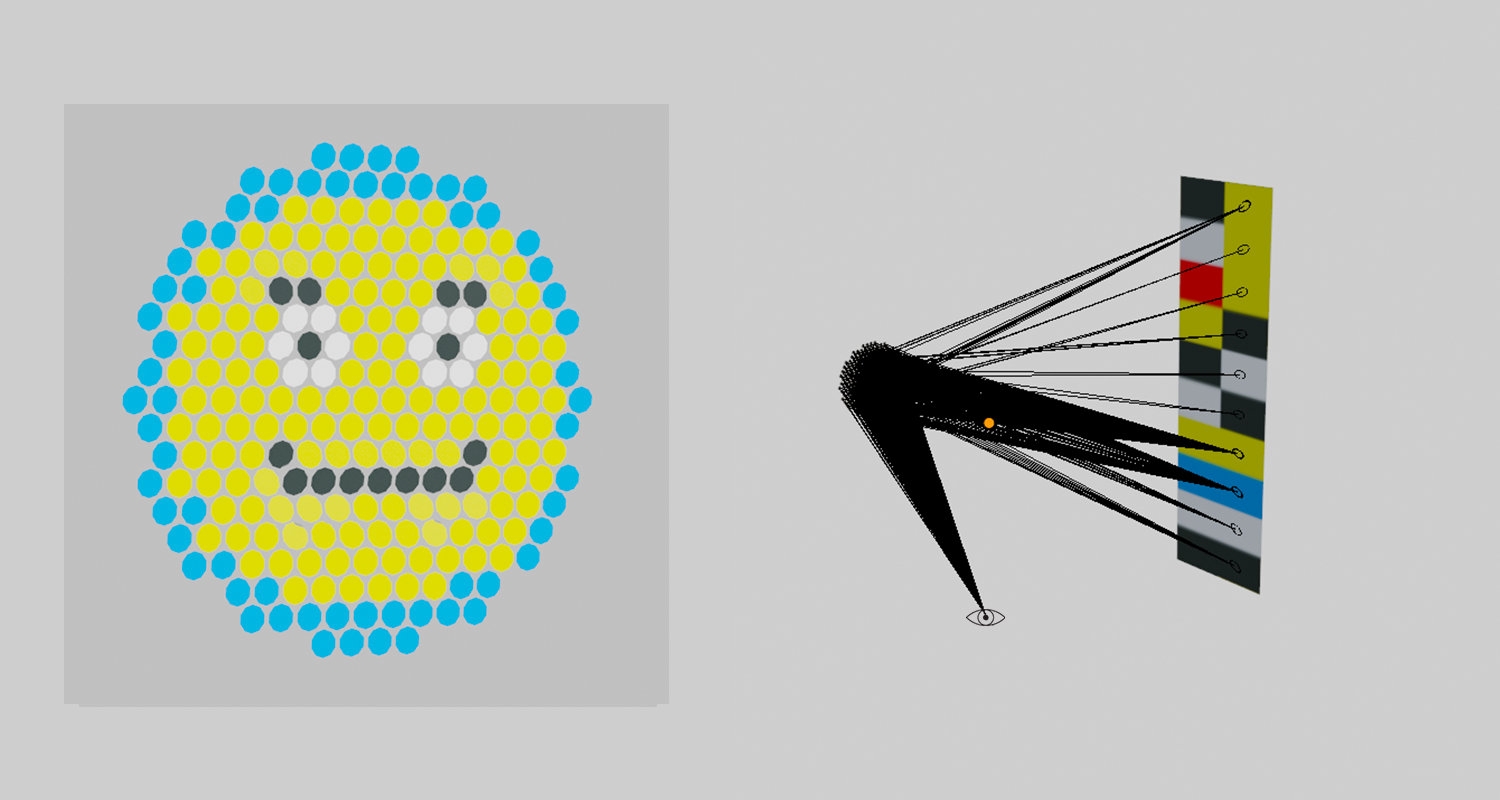
\includegraphics[width=\textwidth]{images/two-image-3d-frame2.png}
\caption{When palette is shifted to the left making the mirrors point to the right column of color fields it produces a second image.}
\label{fig:two_image_3d_frame2}
\end{figure}


In the example in figure \ref{fig:two_image_3d_frame1} and \ref{fig:two_image_3d_frame2} the palette has been shifted slightly to the left
while everything else is left untouched. Even though we use the same
amount of colors we now have ten rows instead of five in the palette.
Each mirror is now assigned a color sequence rather than a single
color. Note that each column of the palette contains some colors
multiple times. In the first image the mirrors depicting the eyebrows
are black but in the second picture the same mirrors are yellow. This
black-yellow color sequence is represented in the first row from the top
of the palette. Further, the mirrors depicting the eyebrows in the
second image are yellow in the first image and black in the second so
those mirrors uses the yellow-black sequence in the fourth row. The red
tongue in the first image disappears in the second image so the red
color only exists once in the first column since all mirrors assigned
red in the first image transitions to yellow in the second.

If we want to add more frames to our animation we could just add another
column. One problem that will be apparent really quickly is that the
more frames we add and the more sequences will be needed to cover all
possible transitions. Adding another column usually also means adding
multiple more rows\footnote{The number of color sequences that can be
  created with \(x\) colors and \(y\) frames is \(x^y\). This means
  that having two colors and five frames will in the worst case (all
  combinations might not be used) make \(5^2 = 25\) rows to be able to
  fit all possible combinations.}. Since the color fields needs to be a
certain physical size the palette has to grow in size with longer
animations and with a larger amount of colors. For longer or more
colorful animations it will become a problem of fitting the palette
into a room.

\section{Some tricks used to optimize and reduce the physical space occupied by the color fields}

A tricky issue for making a good mirror picture keeping the size
down and in particular the size of the color palette. Having more
color fields allows for more complex color sequences and hence more
complex images but it will also require a spatially bigger color
palette or smaller color fields. When the color fields get smaller it
requires a higher precision of the mirrors angles to accurately fit the
frustums base within the color field. Smaller color fields also means
that the rays needs to strike them at an angle close to the normal to
not distort the frustum base. The bigger the color palette fields are
the more viewing position room for error there is so we want to optimize
for as few color fields as possible since that will make more of them
fit in each unit of area. So we want to minimize the number of color
fields since that allows us to maximize their size given the same
overall size.


\subsection{De Bruijn sequences}

From the example with the smileys one can make the observation that one
horizontal sequence might start with the same colors as another ends
with. It might be possible to put all sequences in one long horizontal
line and let some sequences overlap each other reducing the total number
of color fields. The palette would work the same way as before: just
shift it one step to the left to advance one frame. For animations with
more frames there might be an even larger overlap where one sequences
first two colors is the same as another's last two colors etc. If we
keep on overlapping like this we will eventually have something called a \emph{De
Bruijn sequence}. A De Bruijn sequence is a sequence that contains every
possible sub-sequence of a particular length once, and only once. \\
It is actually possible to compute the De Bruijn sequence rather easily
although we will not go into the details of it here but instead just
assume we can do it.

Take for example this naïve sequence that is made up by concatenating all two
letter combinations of A, B , C, D and E (we are using letters here
instead of colors for clarity). Of course it contains all two letter
sub-sequences e.g. AB, DA, BD, DD (below set in bold) etc. since it was
made from it in the first place but we can see that there are multiple
instances of many of the combinations. For example there are more than
one AB (bold) which is redundant.

A A \textbf{A B} A C A D A E B \textbf{A B} B B C B D B E C A C B C C C
D C E D A D B D C D D D E E A E B E C E D E E

Below is the De Bruijn sequence, also containing all two letter
sub-sequences but with the difference that it does not contain any
duplicates and hence is much shorter.

A \textbf{A B} A C A D A E B B C B D B E C C D C E D D E E A

In the first example with the naïve implementation we needed to use
\(y*x^y = 50\) fields (where \(x\) denotes the number of colors and
\(y\) the length of the sub-sequence) while we with a De Bruijn sequence
we only need \(x^y + 1 = 26\) to fit all possible color sequences in the
best case saving about 50\% space.

\begin{figure}[ht!]
\centering

\includegraphics[width=\textwidth]{images/two-image-debruijn-sequence.png}
\caption{The De Bruijn sequence for the example smiley animation above. They eyebrows that used the black-yellow and yellow-black transitions can be found in the middle. Spatially those two sequences takes up only three unit squares while the naïve version uses four, a 25\% saving.}
\end{figure}

Now, we might not actually need all the color fields in the De Bruijn
sequence. There might not be any need for a transition from A to A (e.g.
in the smiley animation there are no transition from red to red) and in
that case we can prune away those sub-sequences and end up with an even
shorter sequence.

The only drawback with using a De Bruijn sequence is that it needs to be
in one continues line which is not very space efficient. We'd like to
have the ratio of the height and the width of the full color palette as
close to \(1.0\) as possible since we get less conic distortions by
having the mirrors set at shallow angles.

\subsection{Disc shaped palettes}

The sequence can be awfully long so it might be an idea to try to pack
the color fields for example in a color circle instead of a color line.
By doing this we will also trade a lot of horizontal space for a little
vertical space making the entire contraption a bit more manageable. This
also means that instead of moving the color fields horizontally we need
to start rotating something\footnote{If the center of the color circle,
  the center of the mirrors and the center of the spectators eye lies on
  the same line we can rotate either the color circle or the mirrors. If
  any of them are not we can only rotate the color circle and still
  produce the effect.}.

\begin{figure}[ht!]
\centering
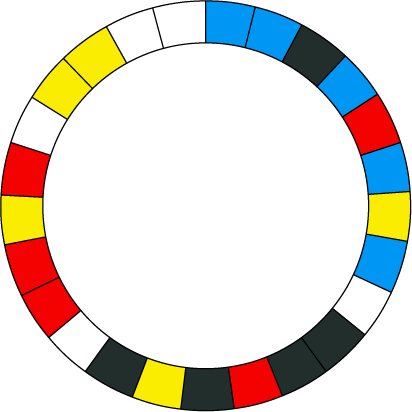
\includegraphics{images/debruijn-wheel.png}
\caption{The smiley animation De Bruijn sequence as a circle.}
\end{figure}


Arranging the De Bruijn sequence in a circle has the small effect that
the sequence is one element shorter than the regular De Bruijn variant
since the last element also works as the first. In the above example the
last blue can be dropped since there is already two blue at the
beginning while still preserving the blue-blue and white-blue
transitions (at 12 o clock in the circle).


\subsection{Loopability and better space utilization}

Even if the De Bruijn sequence is efficient at packing information in a
sequence it's still not great for actual wall space. All the space in
the center is wasted. We could just keep the circle idea but combine it
with the row-column we had in the beginning but wrapping it around a
circle. That would make a color palette disc instead of a circle. We
can advance to the next frame by rotating the disc and if we keep
rotating we'll get back to the first frame again which gives us the nice
feature that the animation loops (see fig. \ref{fig:sequence_wheel_non_sorted}).

\begin{figure}[ht!]
\centering
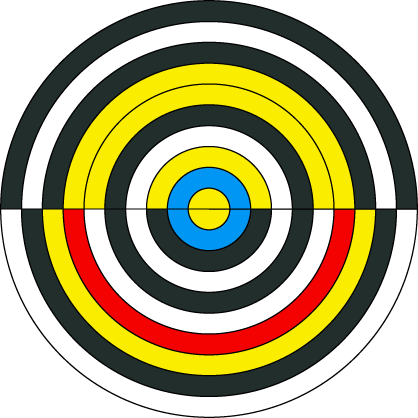
\includegraphics{images/sequence-wheel-non-sorted.png}
\caption{The smiley animation color sequence as a disc.}
\label{fig:sequence_wheel_non_sorted}
\end{figure}



\subsection{Sorting the sequence rings with Shannon entropy}

The radial ordering of the sequences (rings) are practically arbitrary.
The sequences closer to the middle cover a smaller area since the
circumference increases with the radius. Since the mirrors might not be
totally exact due to the fabrication process it can be a good idea to
have more information density in the periphery of the disc where the
area are bigger. We could for example sort the sequences in a way such
as we put the single color sequences end up close to the middle and the
sequences with multiple colors end up close to the periphery. An over
engineered method (that I've opted to go with) is to sort the sequences
by their Shannon entropy \footnote{Shannon entropy of \(X\) is defined as:
\(\eta(X) = -\sum_{i=1}^n {\mathrm{P}(x_i) \log \mathrm{P}(x_i)}\)\\
Where \(x_1, ..., x_n\) is the possible outcomes which occur with
probability \(\mathrm{P}(x_1), ..., \mathrm{P}(x_n)\).}.
We don't really have to dwell too long on the nitty gritty but can
conclude we can compute a number for each sequence that will be
different when not much happens compared to when a lot is happening. We
can then use that to sort the radial rings. In our example here single
color sequences ends up in the middle. In practice this means that the
sequences with less transitions end up in the middle of the circle and
the ones with a lot of transitions end up at the periphery.

\begin{figure}[ht!]
\centering
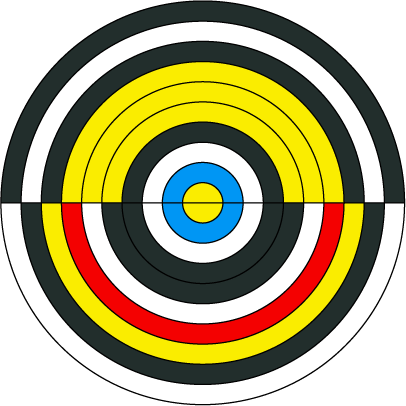
\includegraphics{images/sequence-wheel.png}
\caption{The smiley animation color sequence with the rings sorted on Shannon entropy.}
\end{figure}



\subsection{Increasing frame-rate by multiplication}

The sequence loops every full revolution of the disc. To make the frame
rate higher without spinning the disc faster we can multiply the color
fields in each radial section. Since the sequence is looping anyway we
haven't in effect made any changes to it. A nice side effect is that the
disc can look slightly more interesting.

\begin{figure}[ht!]
\centering
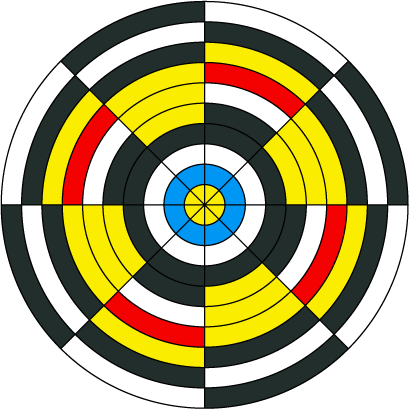
\includegraphics{images/sequence-wheel-frame-duplicate.png}
\caption{The smiley animation color sequence with the elements of the sequences multiplied four times.}
\end{figure}



\subsection{Prune redundancies}

After sequence multiplication it is obvious that a few sequences are
redundant. In our example we have the black-white transition that is
topologically equal to the white-black transition. The same goes for the
black-yellow and yellow-black transitions. We can just assign each
mirror a sequence with a starting offset and drop the duplicate. For
example to get the black-white sequence we can aim a mirror the first
black field starting from 0° on the disc. To assign the white-black
sequence we just skip ahead a bit and aim it the first white field. The
first frame will then be black or white respectively and when rotating
the disc we advance to the next color in the sequence being white and
black respectively. Since there are multiple valid starting offsets
(depending on how many times we did the sequence multiplication) we can
actually just assign any valid one at random for each mirror.

\begin{figure}[ht!]
\centering
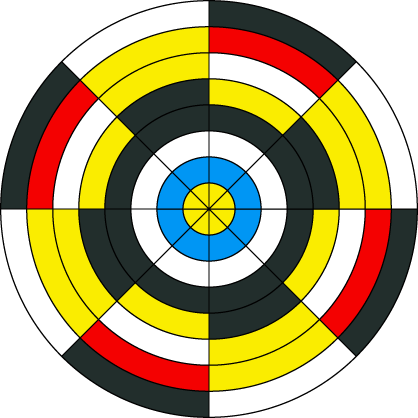
\includegraphics{images/sequence-wheel-removed-redundancies.png}
\caption{The smiley animation color sequence with topologically similar sequences pruned.}
\end{figure}



\subsection{Ring staggering}

If we think that the disc looks a bit static we can introduce some
rotational shift between each ring radially. This doesn't affect the
sequence but gives us some artistic flexibility.

\begin{figure}[ht!]
\centering
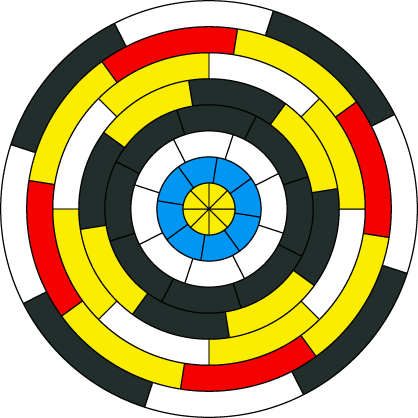
\includegraphics{images/sequence-wheel-helix-shift.png}
\caption{The smiley animation color sequence with each radial ring shifted 3.7° in relation to the next ring.}
\end{figure}

\subsection{Not overlapping pictures}

As we have seen in previous optimizations it is possible to reduce the
number of color fields used to encode a sequence but it is even better
to keep the number of sequences down to begin with. Making animations constructed
in a certain way can make the number of sequences be equal to the number
of colors regardless of how many frames there are. Imagine that all
images in all frames have one smaller image in it with a solid
background color around it. The position of the smaller image in each
frame only overlaps the background in the other frames. This leads that
each mirror is assigned a sequence that contains one element with a
color and all other elements are just the background color. With the
pruning redundancies trick above we can collapse the number of sequences
to one per color no matter how many colors or frames there is.

\begin{figure}[ht!]
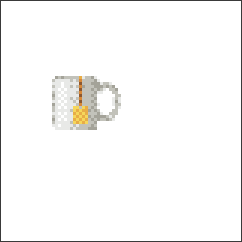
\includegraphics[width=0.3\textwidth]{images/tea-sun-lager-0.png}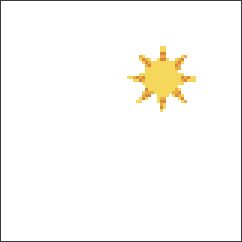
\includegraphics[width=0.3\textwidth]{images/tea-sun-lager-1.png}
\includegraphics[width=0.3\textwidth]{images/tea-sun-lager-2.png}
\caption{Three frame animation where each frame contains a smaller image that doesn't overlap.}
\end{figure}

In the above animation of three frames has three objects placed on a
solid white background. It is made out of eleven colors. If the objects
would all overlap it would in the worst case end up being 1331 different
sequences to cover all possible transitions that would have to fit in
the palette. Without the overlapping images we only need 11 sequences to
cover all possible transitions (again, the same as the number of
colors). There are for example no grey-yellow-orange transition or
brown-yellow-yellow there is just color-white-white. Adding another
frame would not add more sequences since it would just make all
sequences be color-white-white-white etc.

\begin{figure}[ht!]
\centering
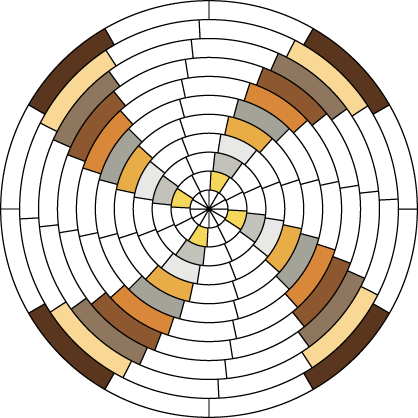
\includegraphics{images/tea-sun-lager-disc.png}
\caption{Palette for the above "tea, sun and lager" animation with four times frame rate multiplication and some staggering.}
\end{figure}



\subsection{Pruning when having too many sequences}

Sometimes the number of colors and/or frames are too high and we end up
with too many sequences even after all previously described
optimizations. When there are too many sequences it is hard to fit all
of them in any given space. One last resort can then be to compromise
and try to prune sequences that are rarely used and replace them with a
substitute that are very similar.

The algorithm reduces the number of sequences until we have the desired
number of sequences. When reducing, some colors will be completely
discarded since they might have very similar approximates already in the
set of sequences (see fig. \ref{fig:reducing}). For example a light brown to red transition can maybe
be replaced with a slightly darker brown to red transition without much
of a visual difference overall. It can also be that a single mirror is
assigned to a sequence and then we can assign that mirror to a sequence
that looks quite similar without it being easy to even notice it. Though
when the number of sequences gets too low ghosting artifacts starts to
appear. Ghosting is when features of one image starts leaking into the
other. In future work this algorithm could probably be improved to avoid
ghosting by for example incorporating more advanced error diffusion
techniques like \emph{Floyd-Steinberg dithering} or \emph{Atkinson
dithering} adapted to work on sequences.

\begin{figure}[ht!]

\centering
\begin{subfigure}[t]{0.4\textwidth}
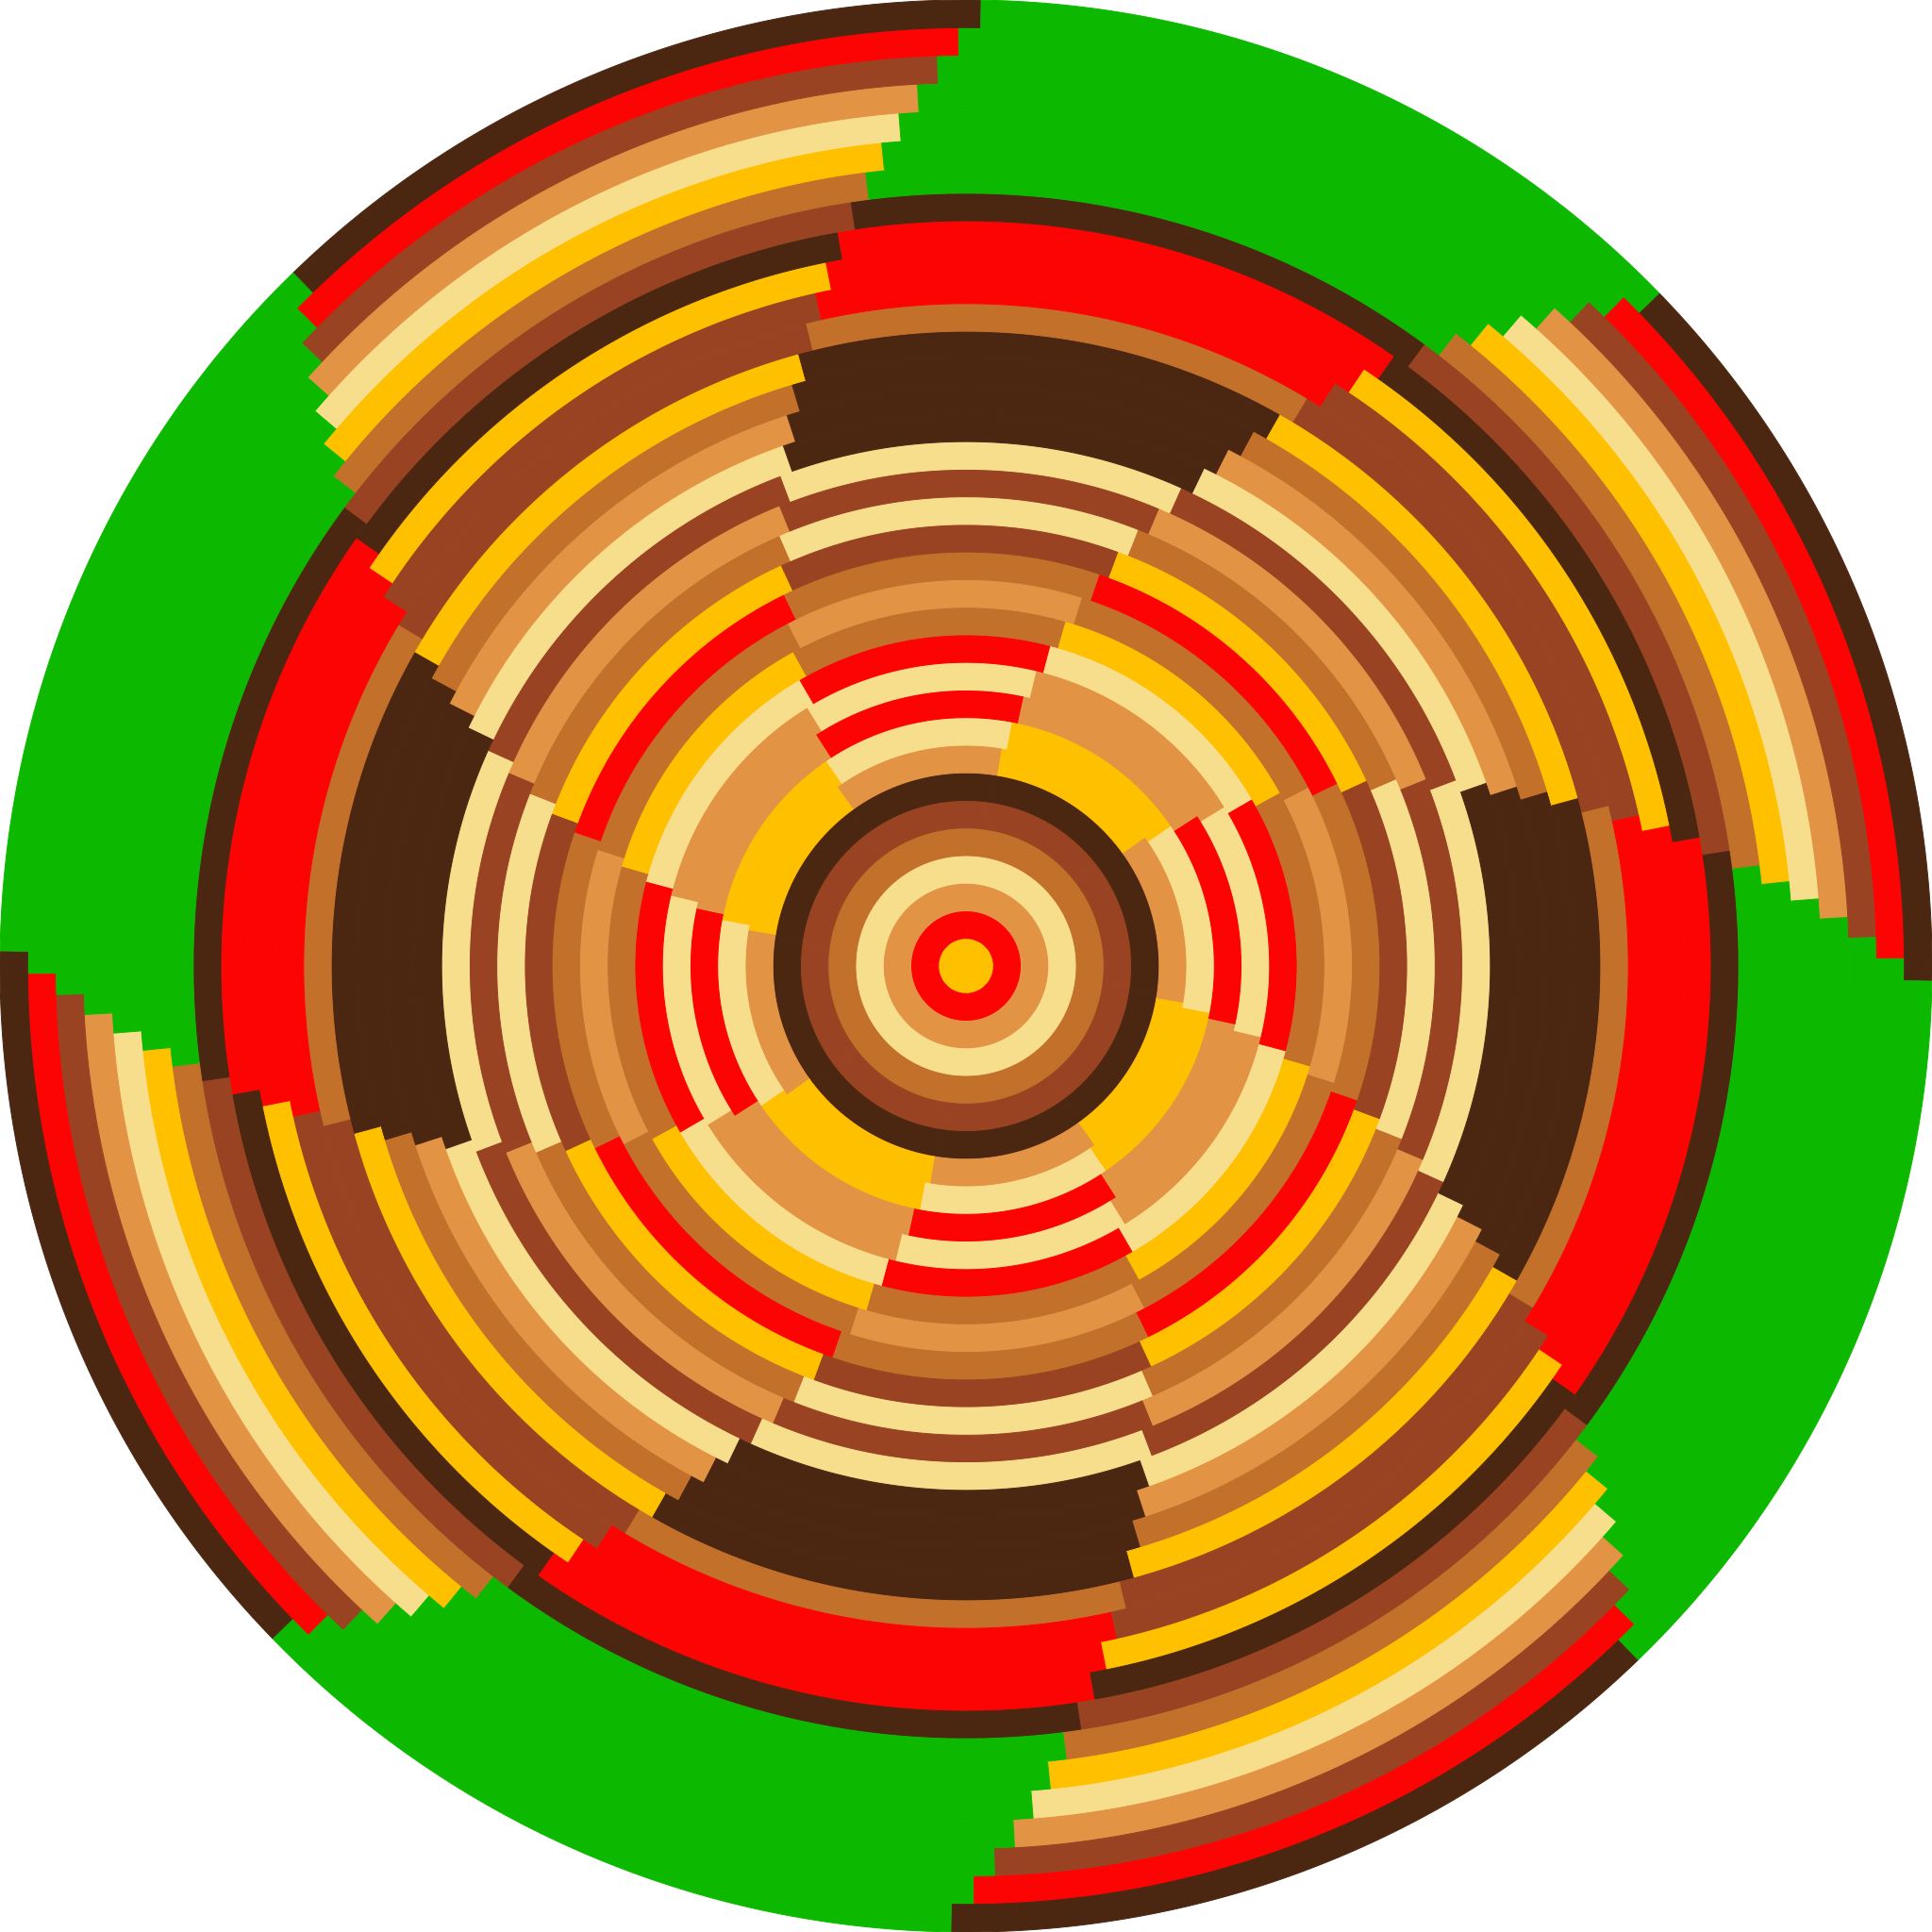
\includegraphics[width=0.3\textwidth]{images/reduction/35/disc.png}
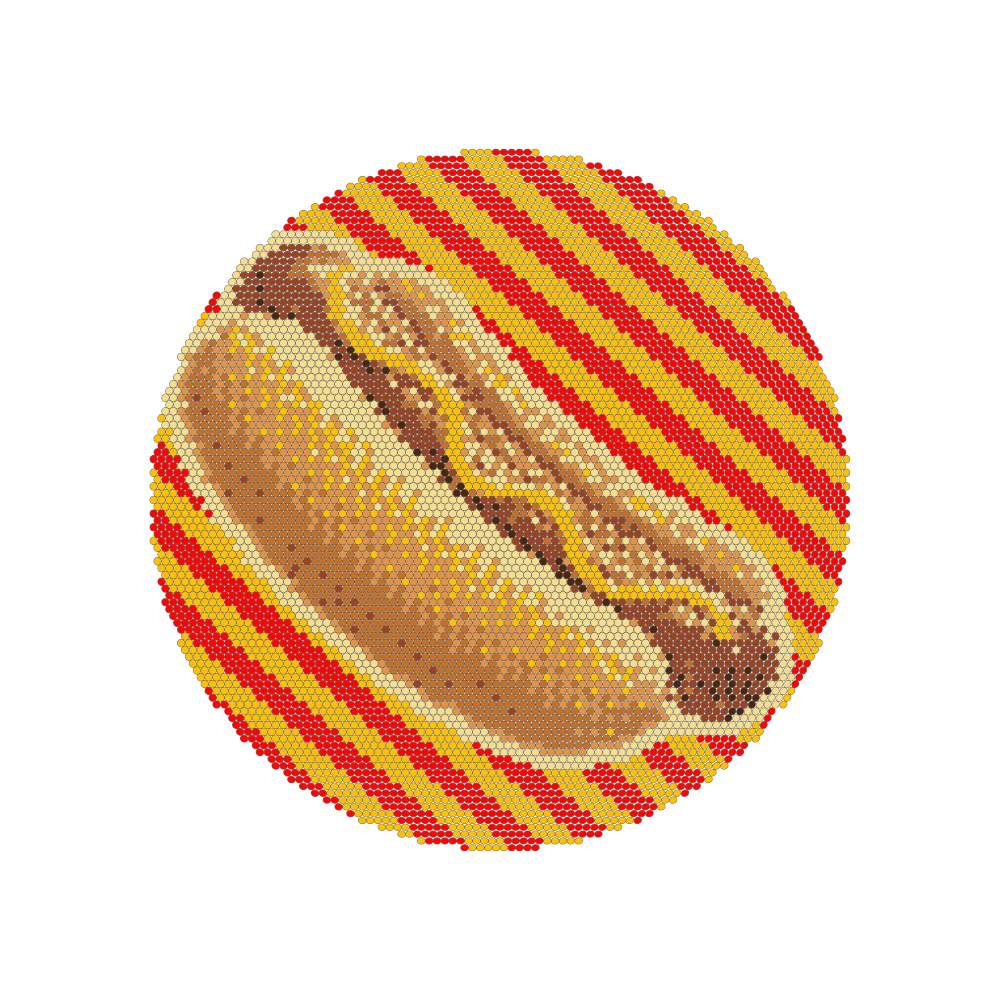
\includegraphics[width=0.3\textwidth]{images/reduction/35/sim0.png}
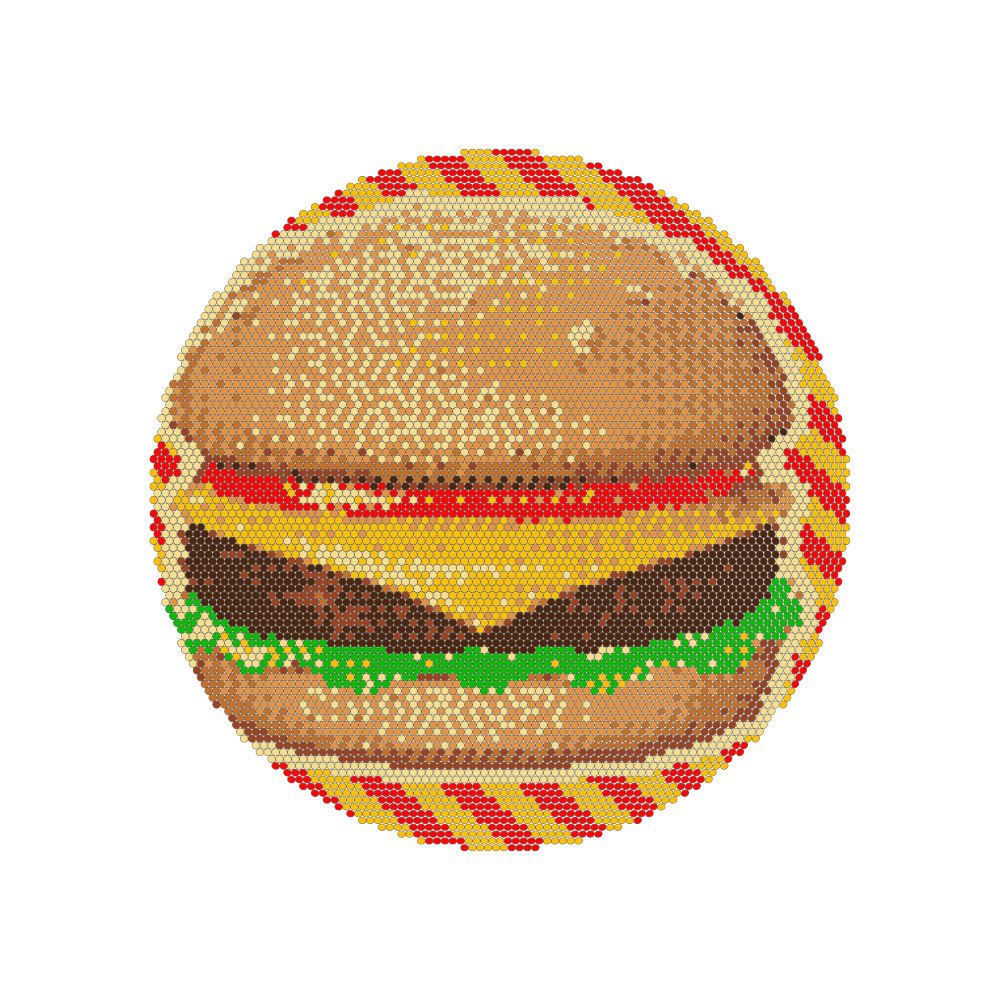
\includegraphics[width=0.3\textwidth]{images/reduction/35/sim1.png}
\caption{35 sequences}
\end{subfigure}
\hfill
\begin{subfigure}[t]{0.4\textwidth}
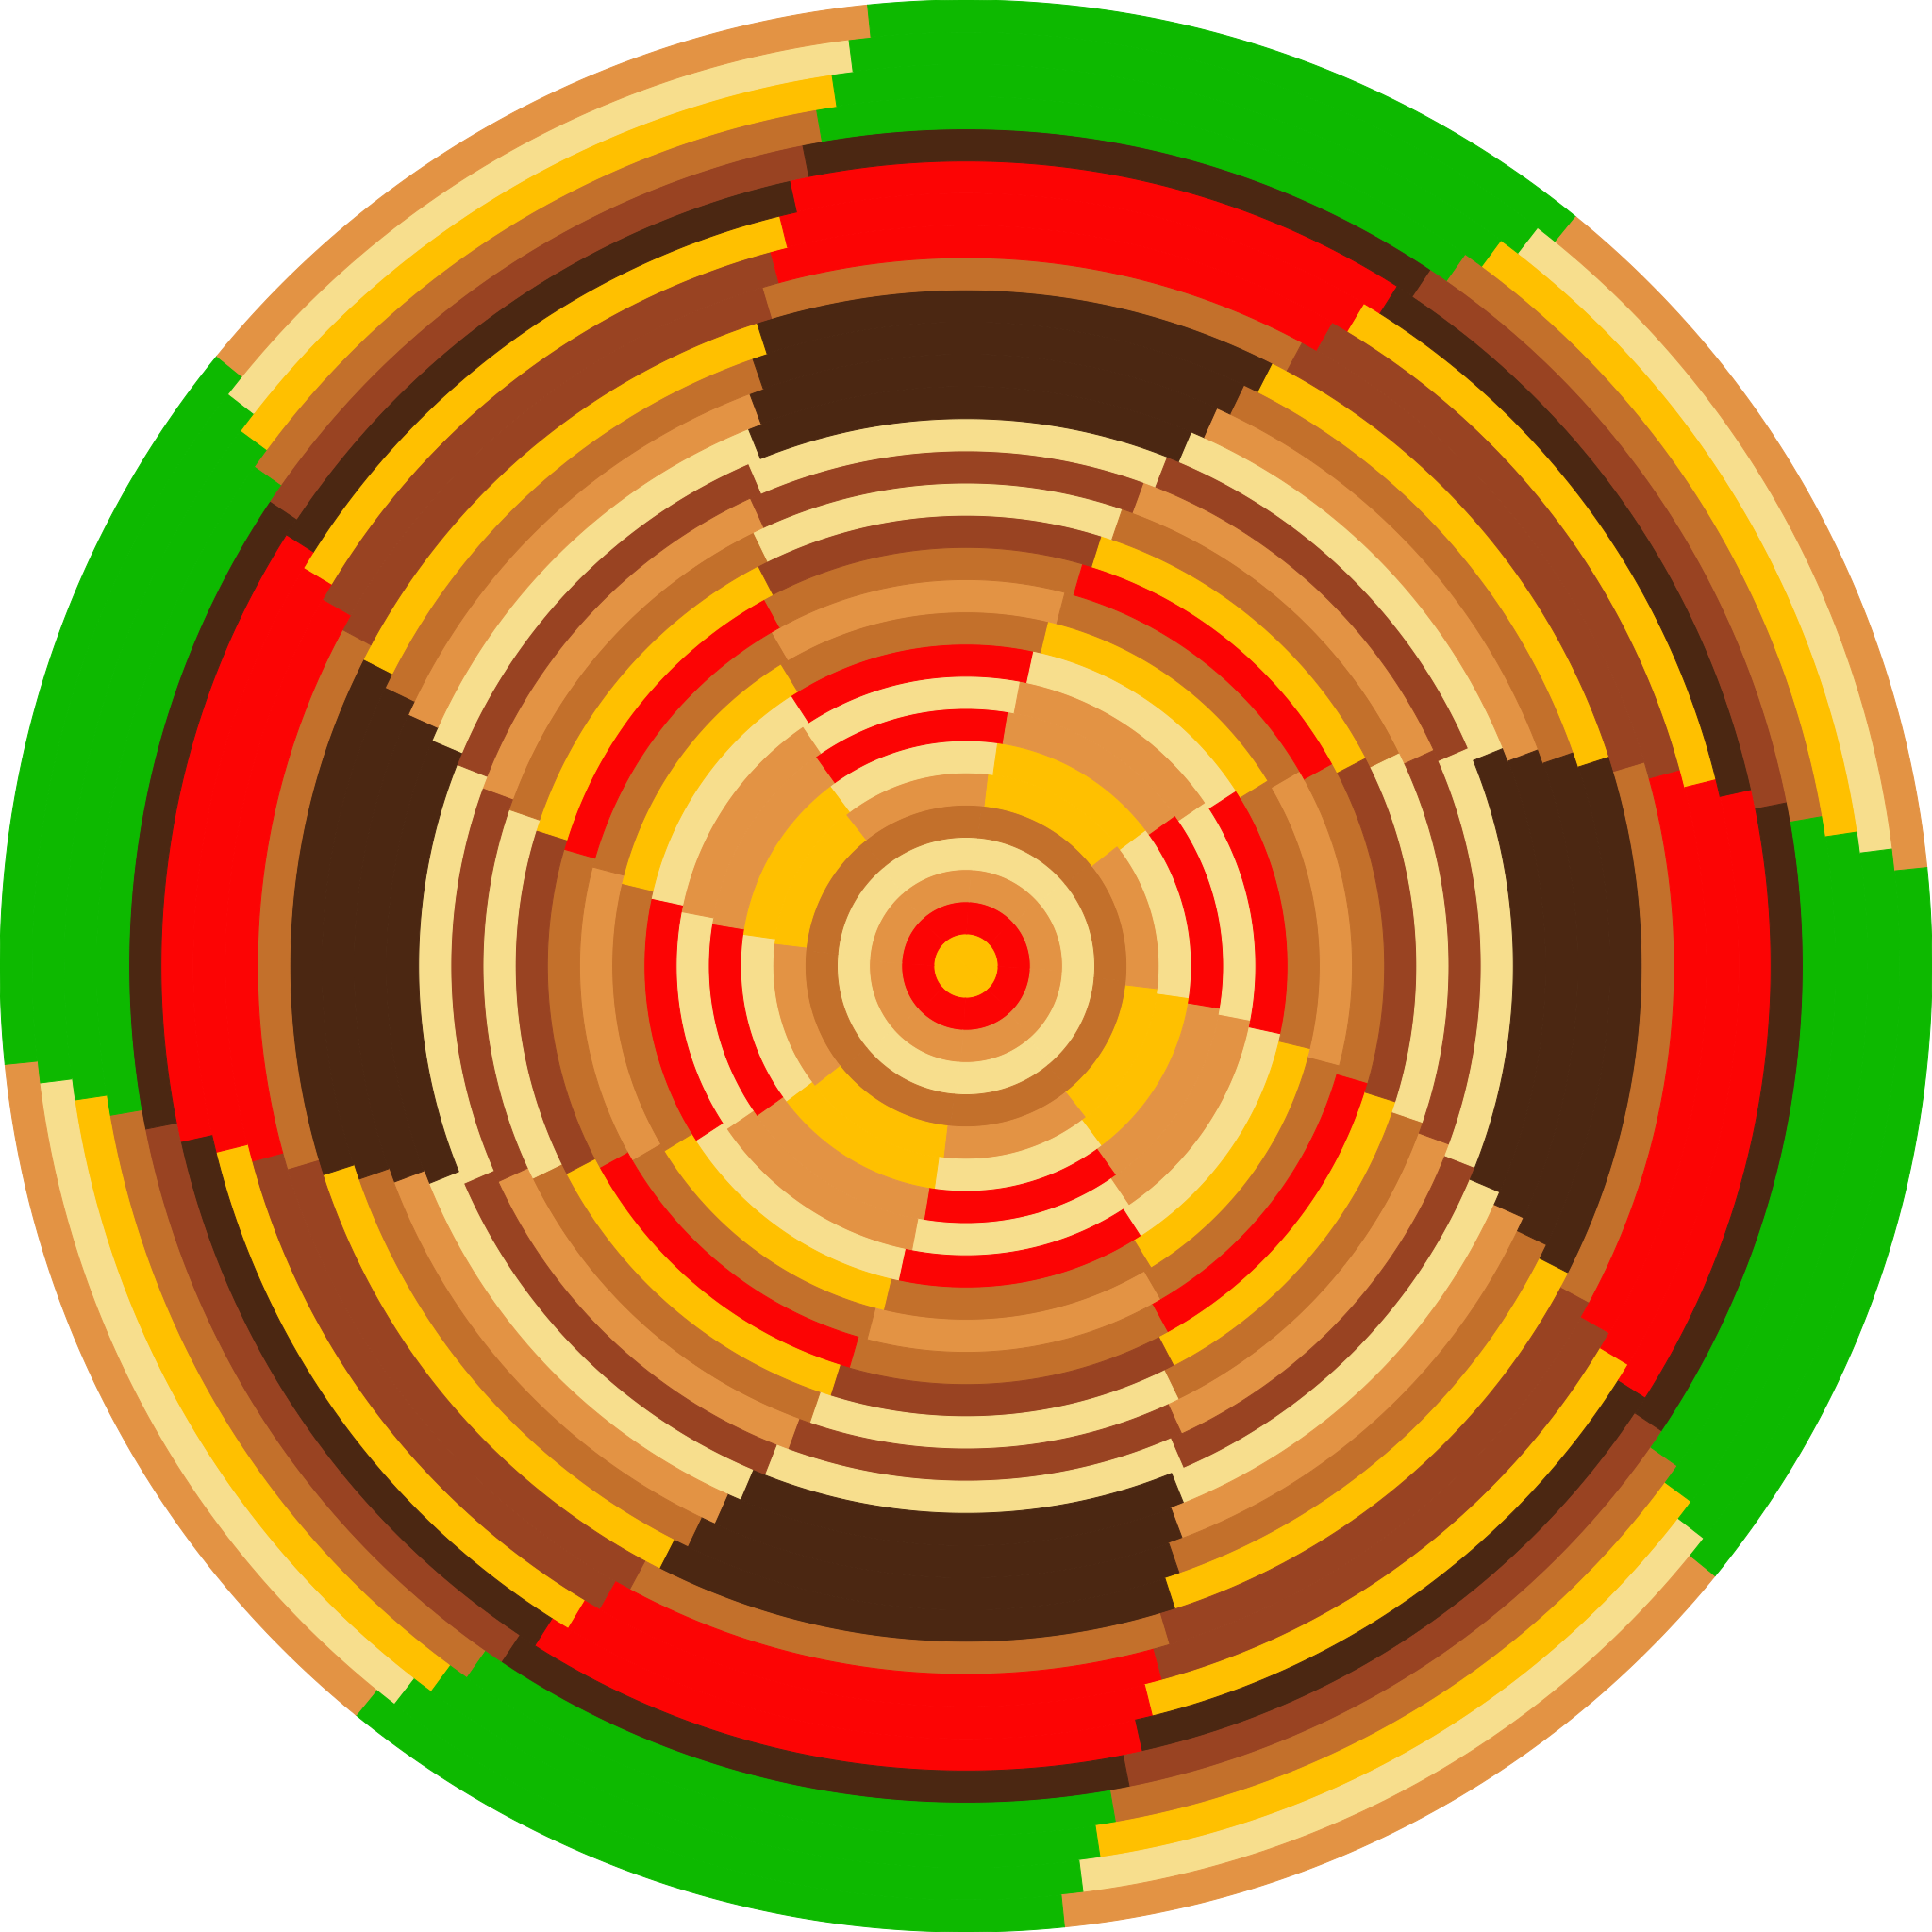
\includegraphics[width=0.3\textwidth]{images/reduction/30/disc.png}
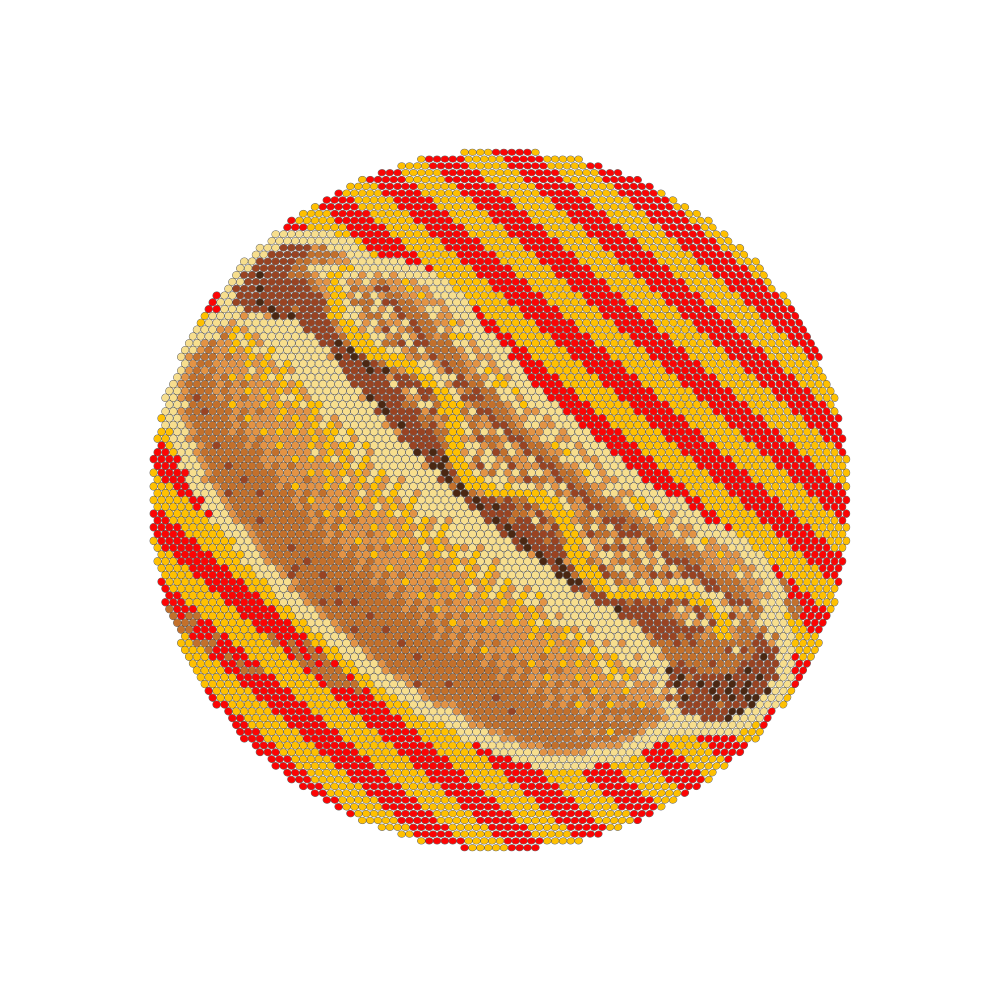
\includegraphics[width=0.3\textwidth]{images/reduction/30/sim0.png}
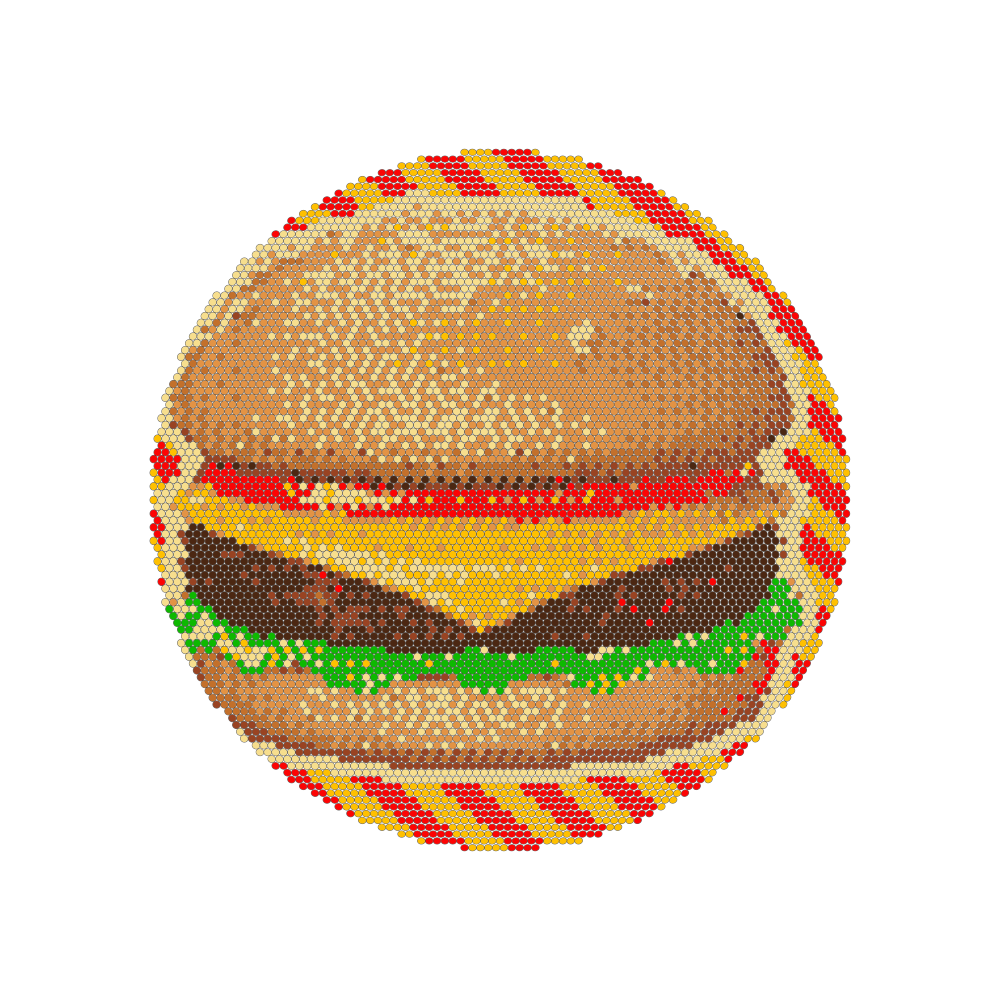
\includegraphics[width=0.3\textwidth]{images/reduction/30/sim1.png}
\caption{30 sequences}
\end{subfigure}

%\end{figure}
%\begin{figure}[ht!]
%\ContinuedFloat

\begin{subfigure}[t]{0.4\textwidth}
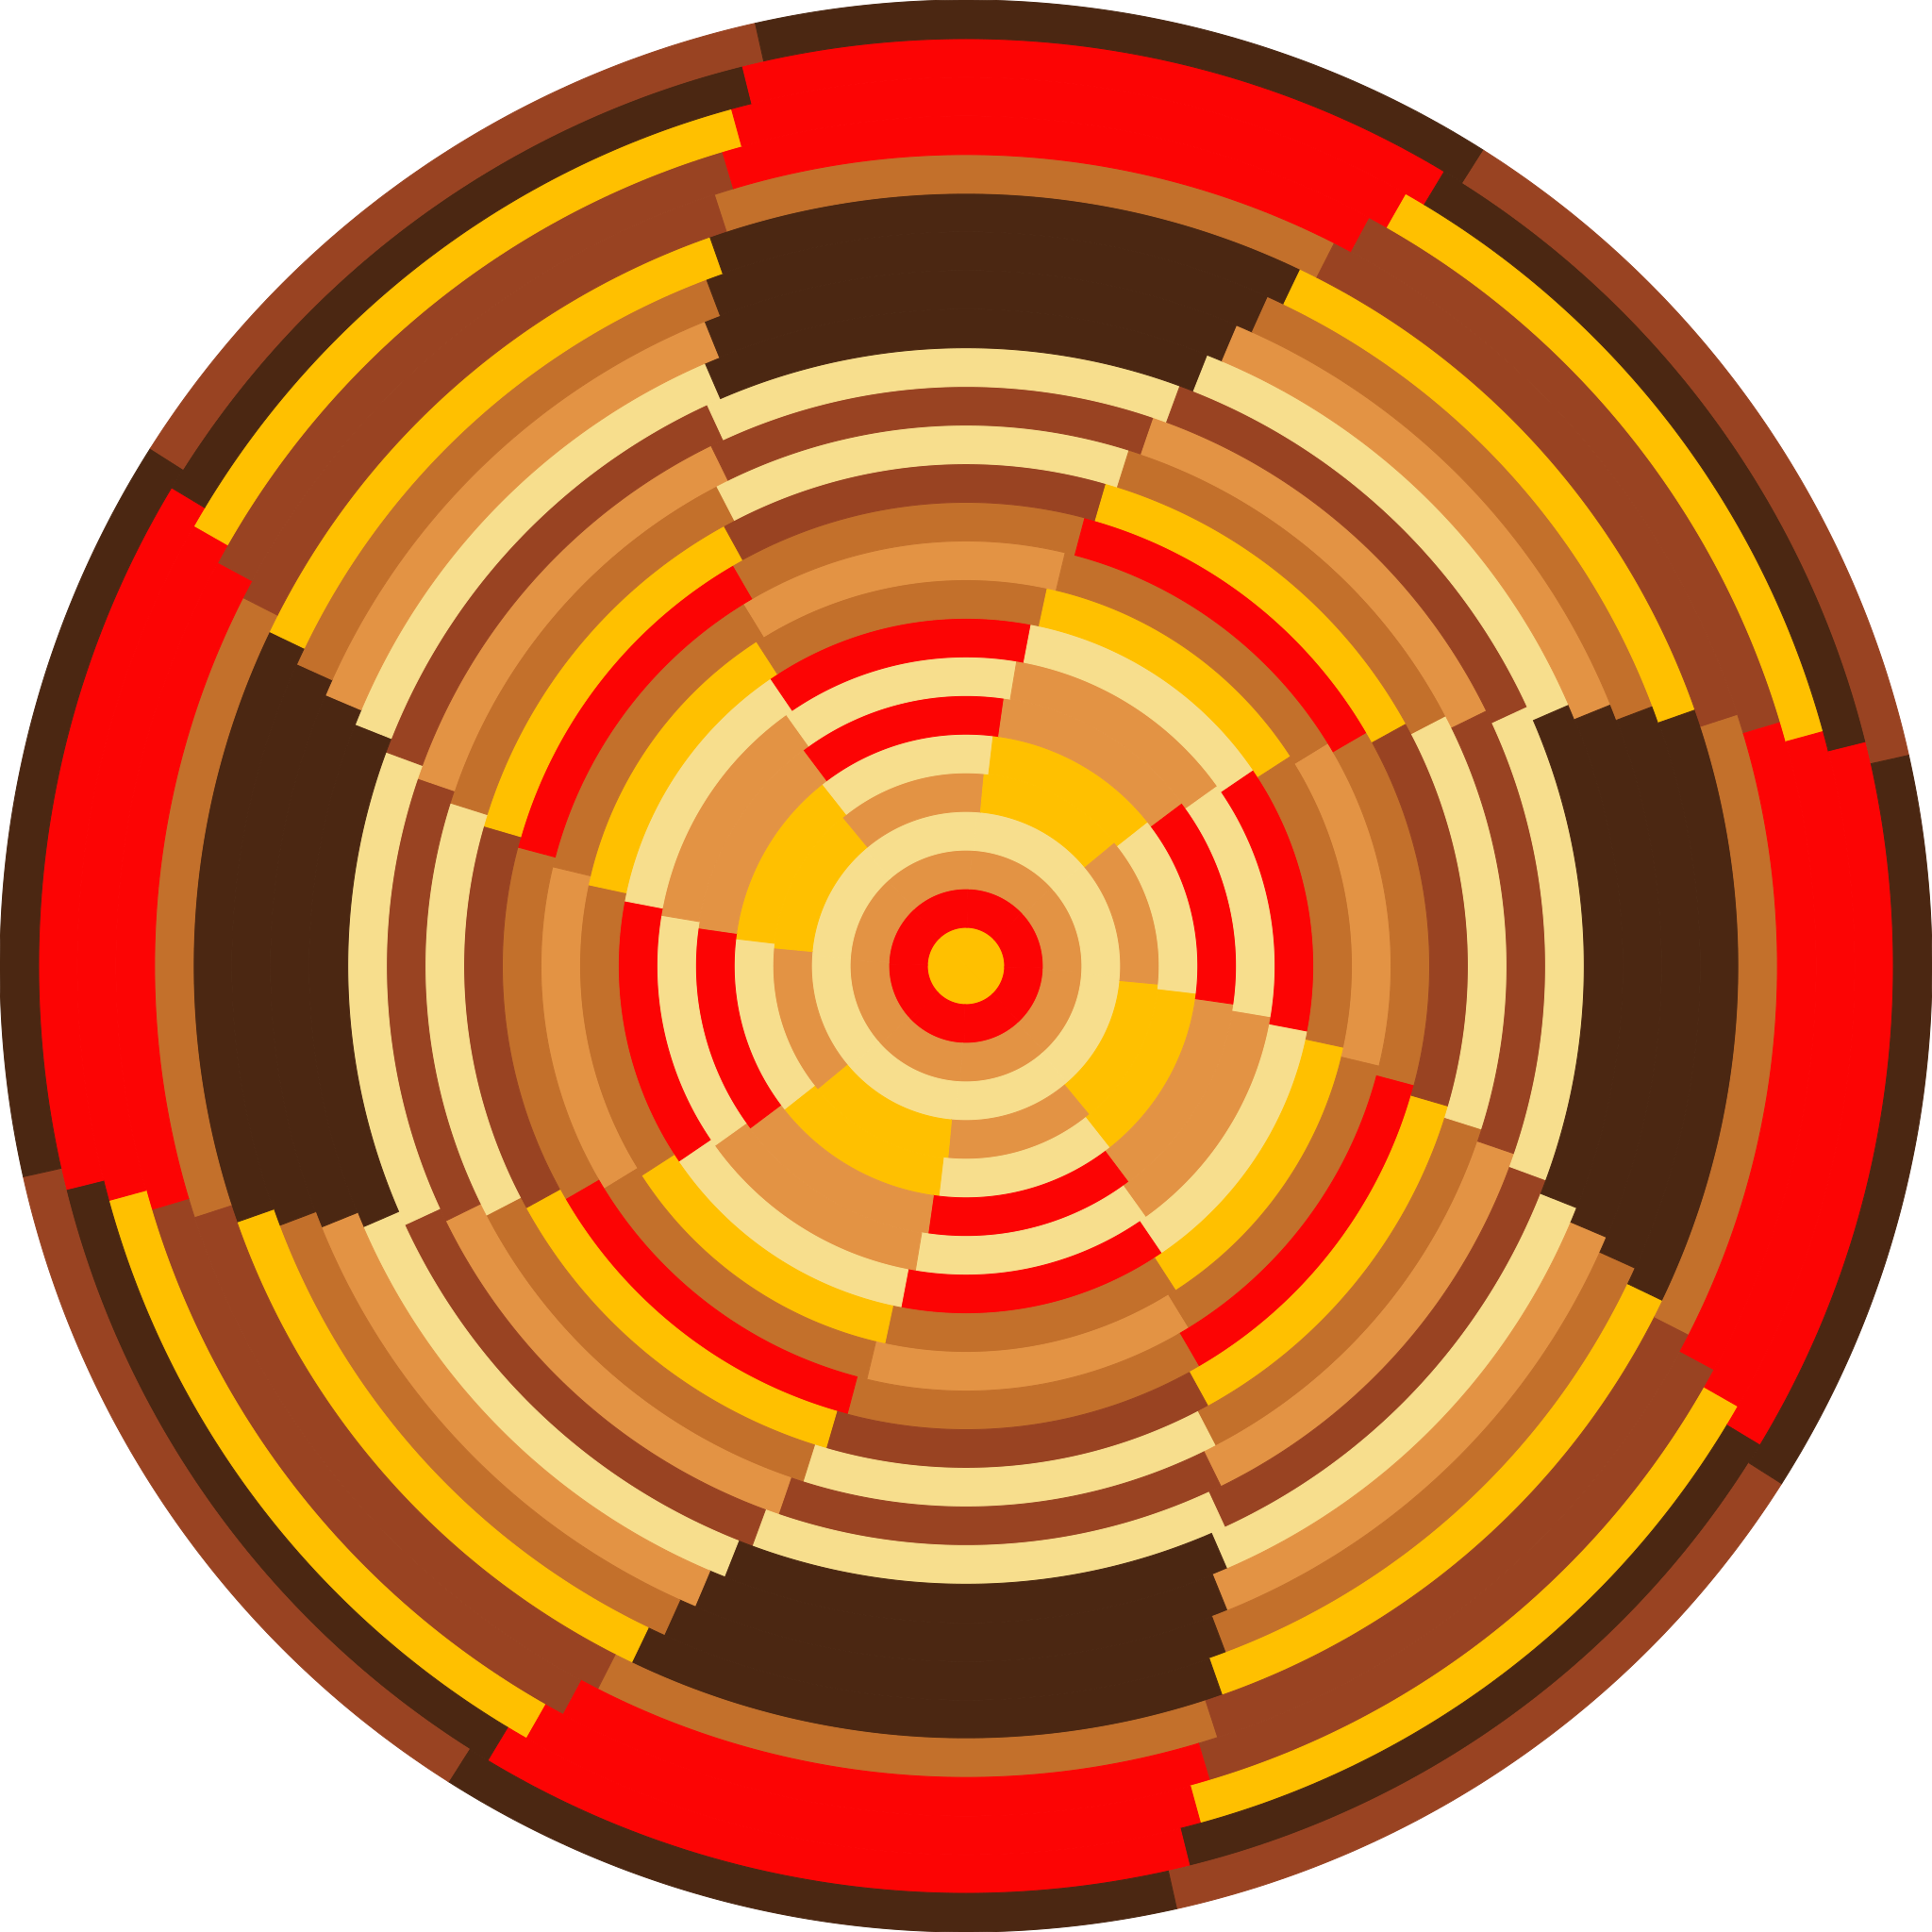
\includegraphics[width=0.3\textwidth]{images/reduction/25/disc.png}
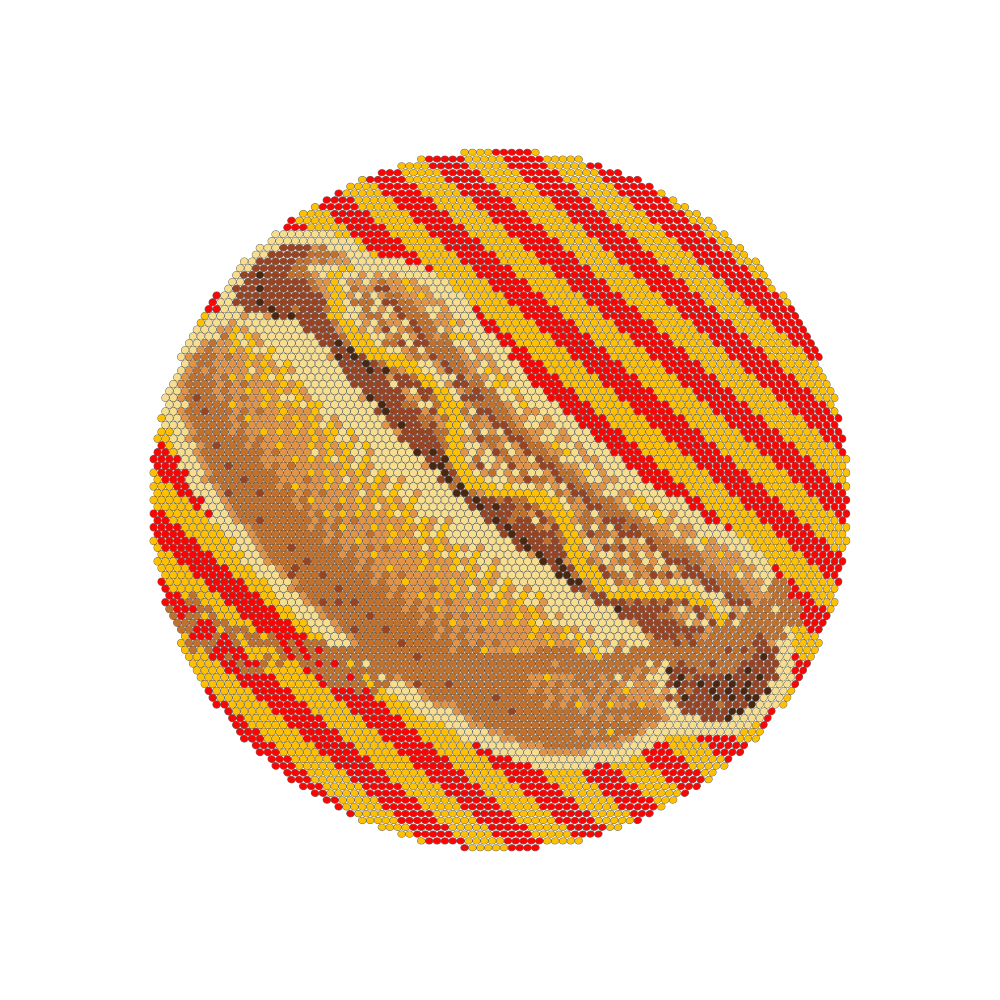
\includegraphics[width=0.3\textwidth]{images/reduction/25/sim0.png}
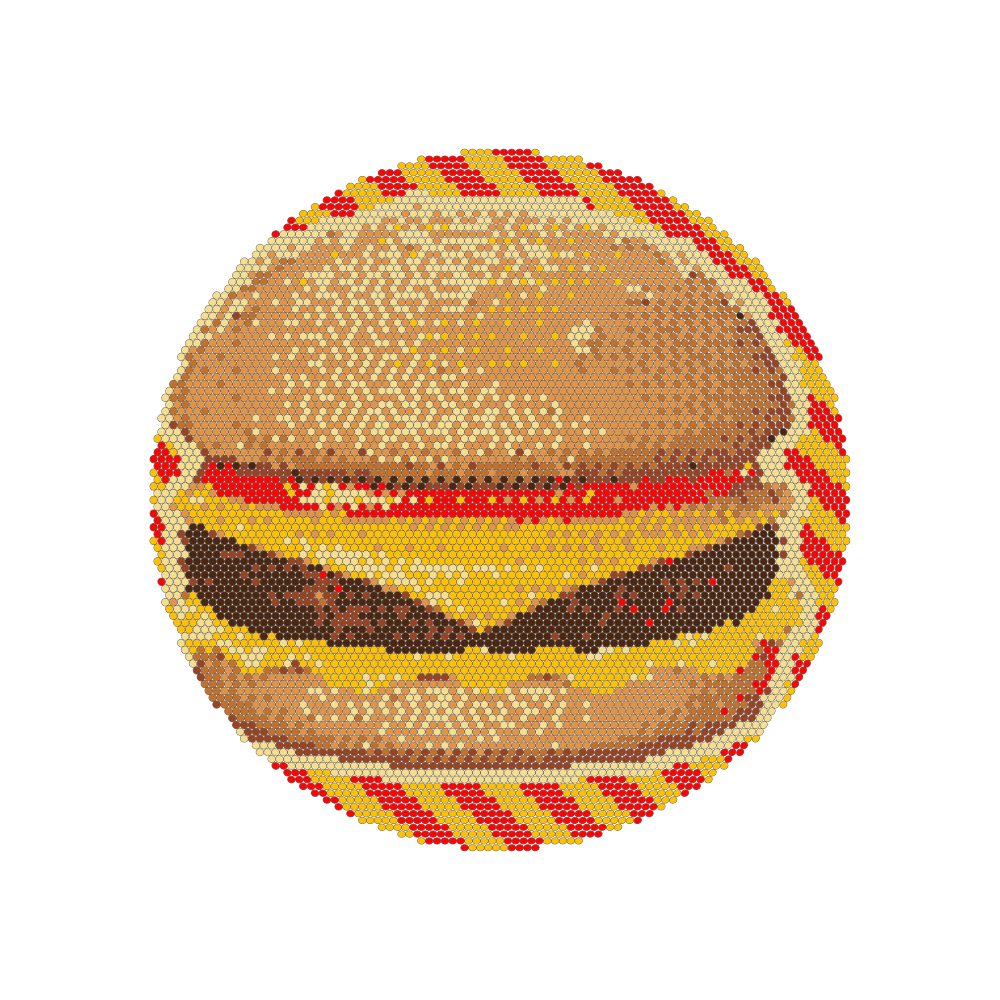
\includegraphics[width=0.3\textwidth]{images/reduction/25/sim1.png}
\caption{25 sequences}
\end{subfigure}
\hfill
\begin{subfigure}[t]{0.4\textwidth}
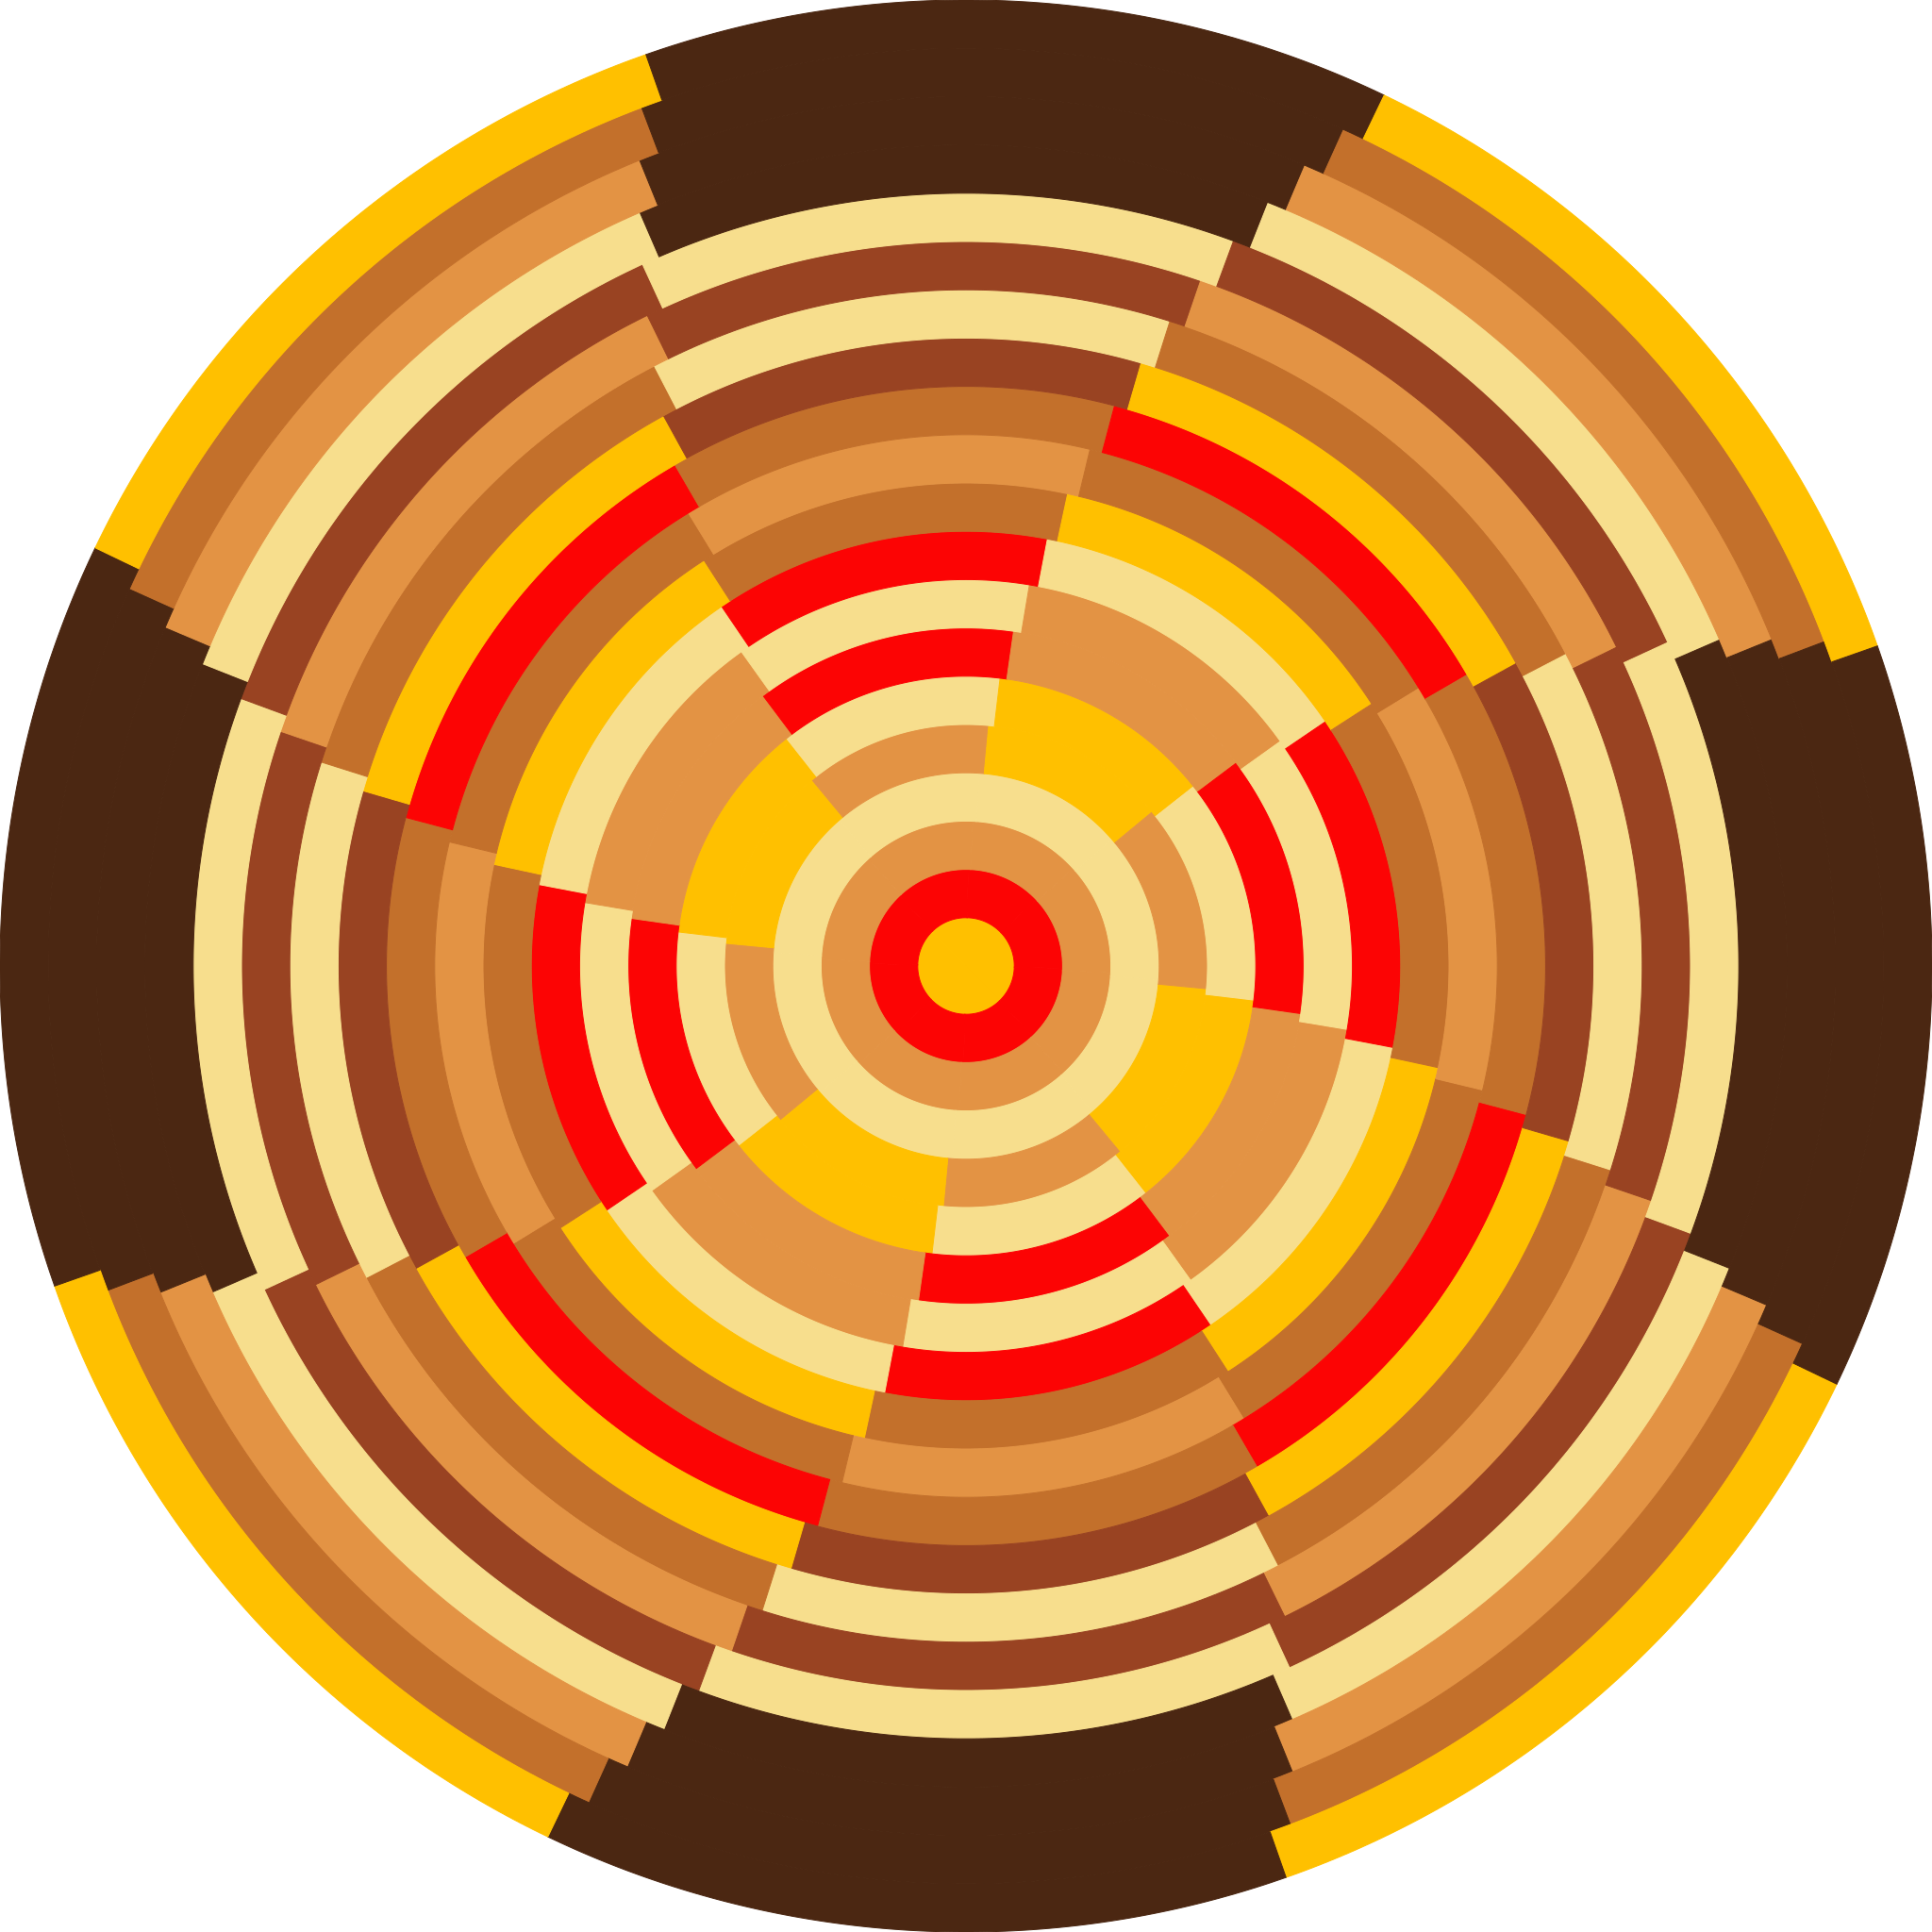
\includegraphics[width=0.3\textwidth]{images/reduction/20/disc.png}
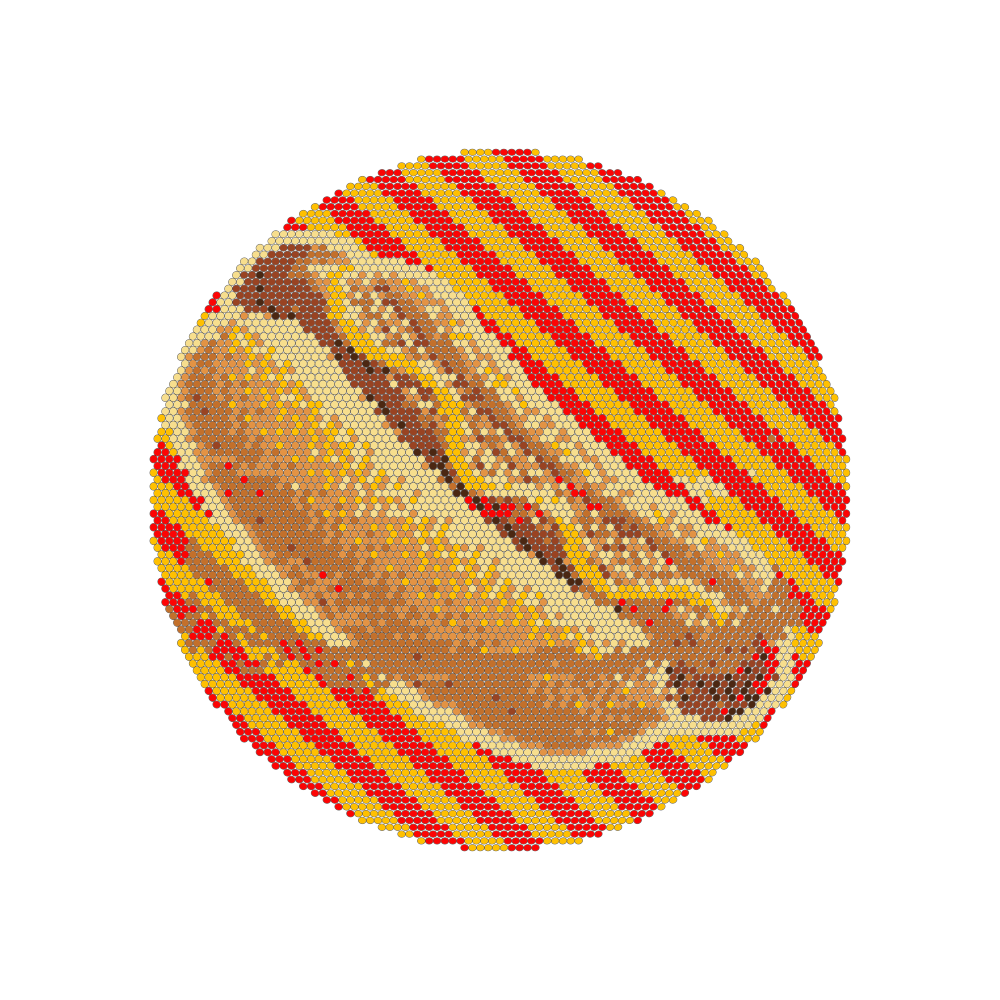
\includegraphics[width=0.3\textwidth]{images/reduction/20/sim0.png}
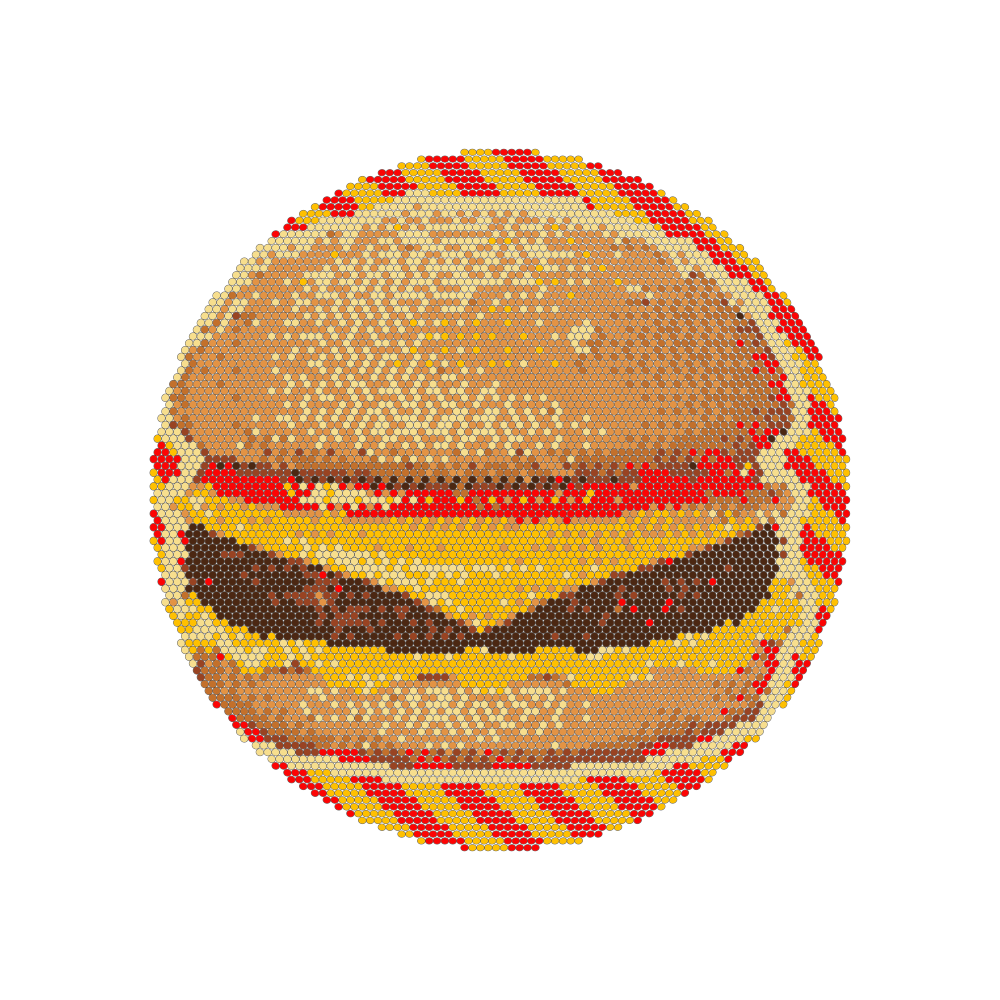
\includegraphics[width=0.3\textwidth]{images/reduction/20/sim1.png}
\caption{20 sequences}
\end{subfigure}

%\end{figure}
%\begin{figure}[ht!]
%\ContinuedFloat

\begin{subfigure}[t]{0.4\textwidth}
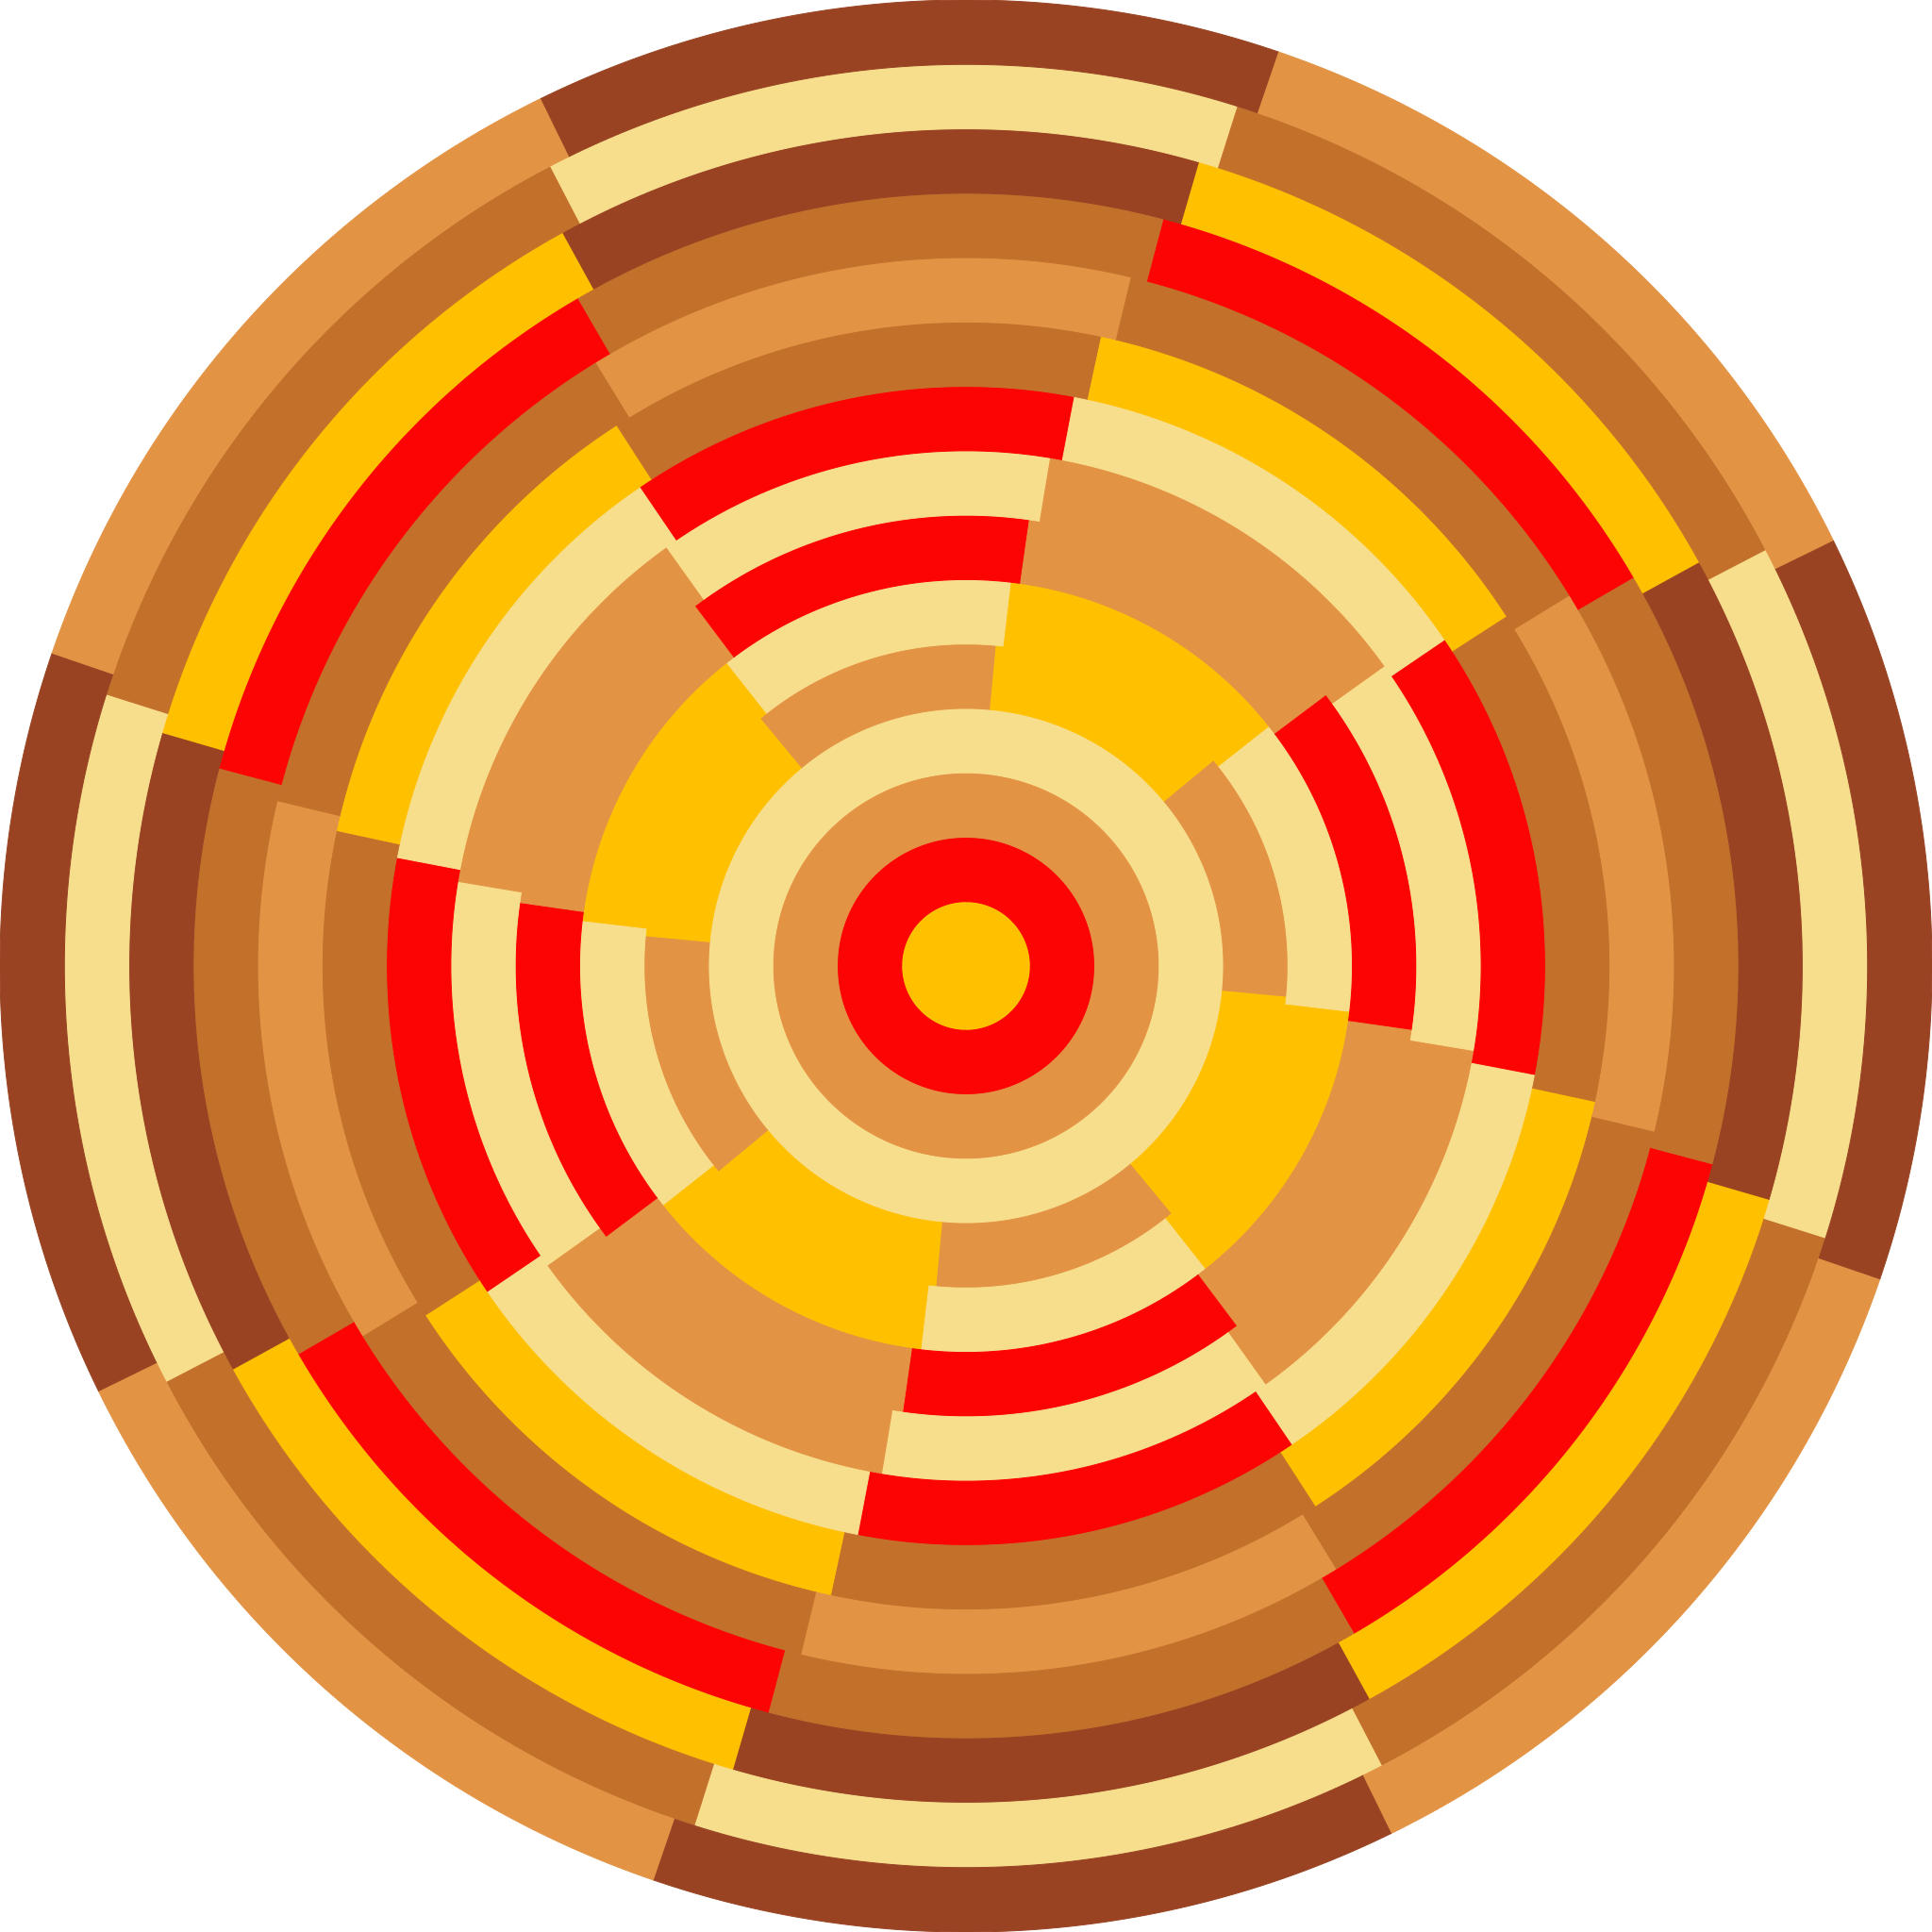
\includegraphics[width=0.3\textwidth]{images/reduction/15/disc.png}
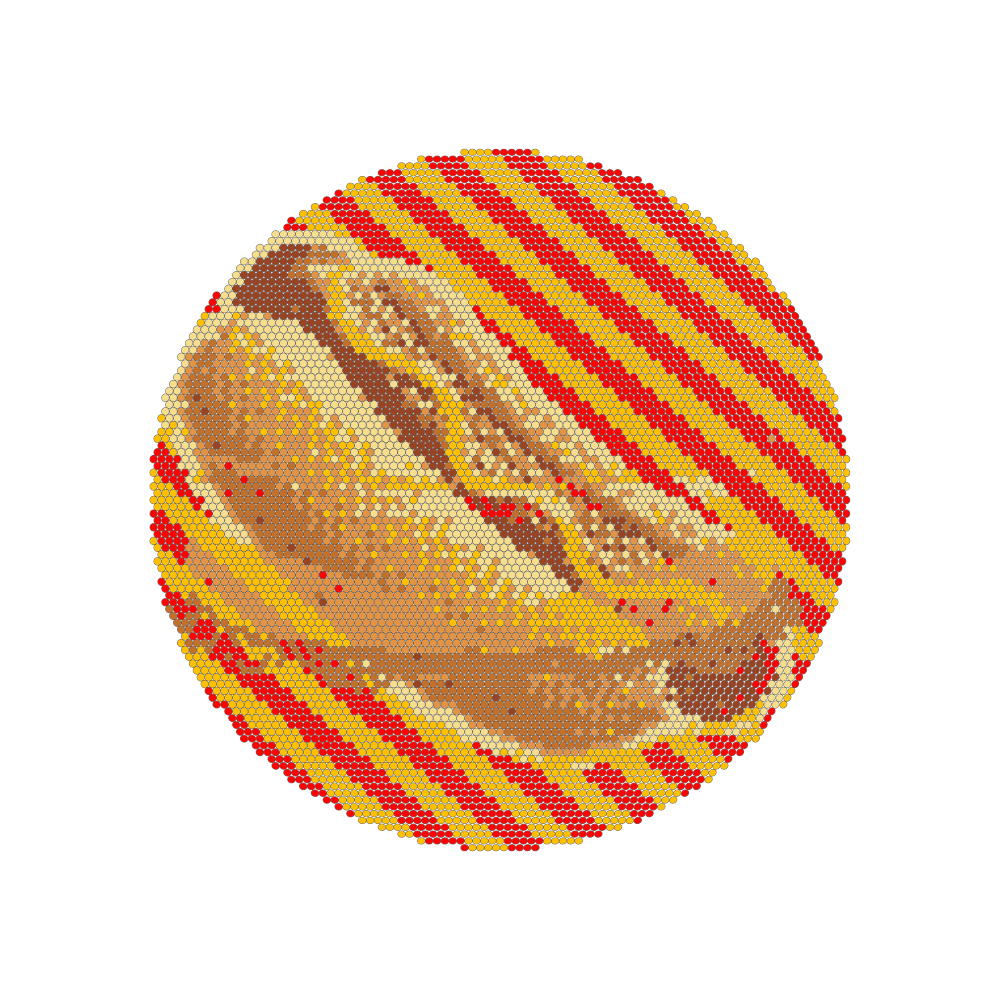
\includegraphics[width=0.3\textwidth]{images/reduction/15/sim0.png}
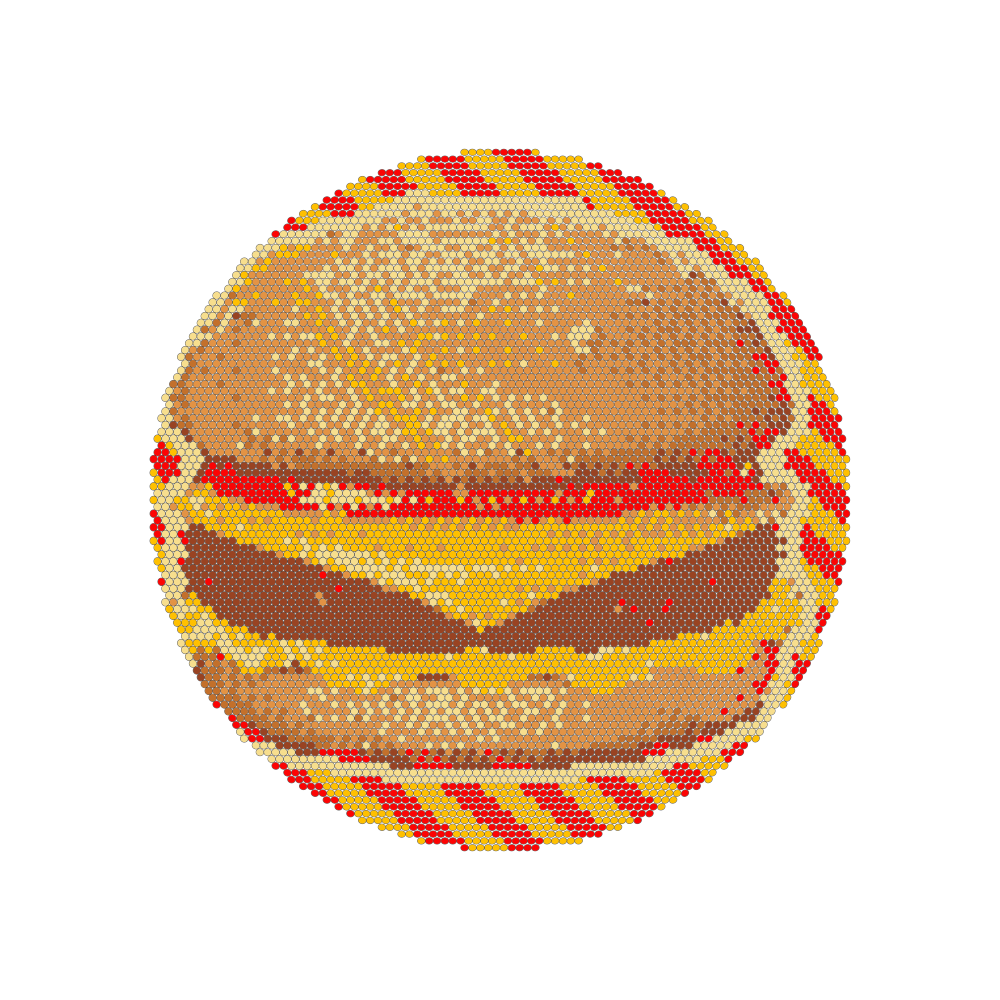
\includegraphics[width=0.3\textwidth]{images/reduction/15/sim1.png}
\caption{15 sequences}
\end{subfigure}
\hfill
\begin{subfigure}[t]{0.4\textwidth}
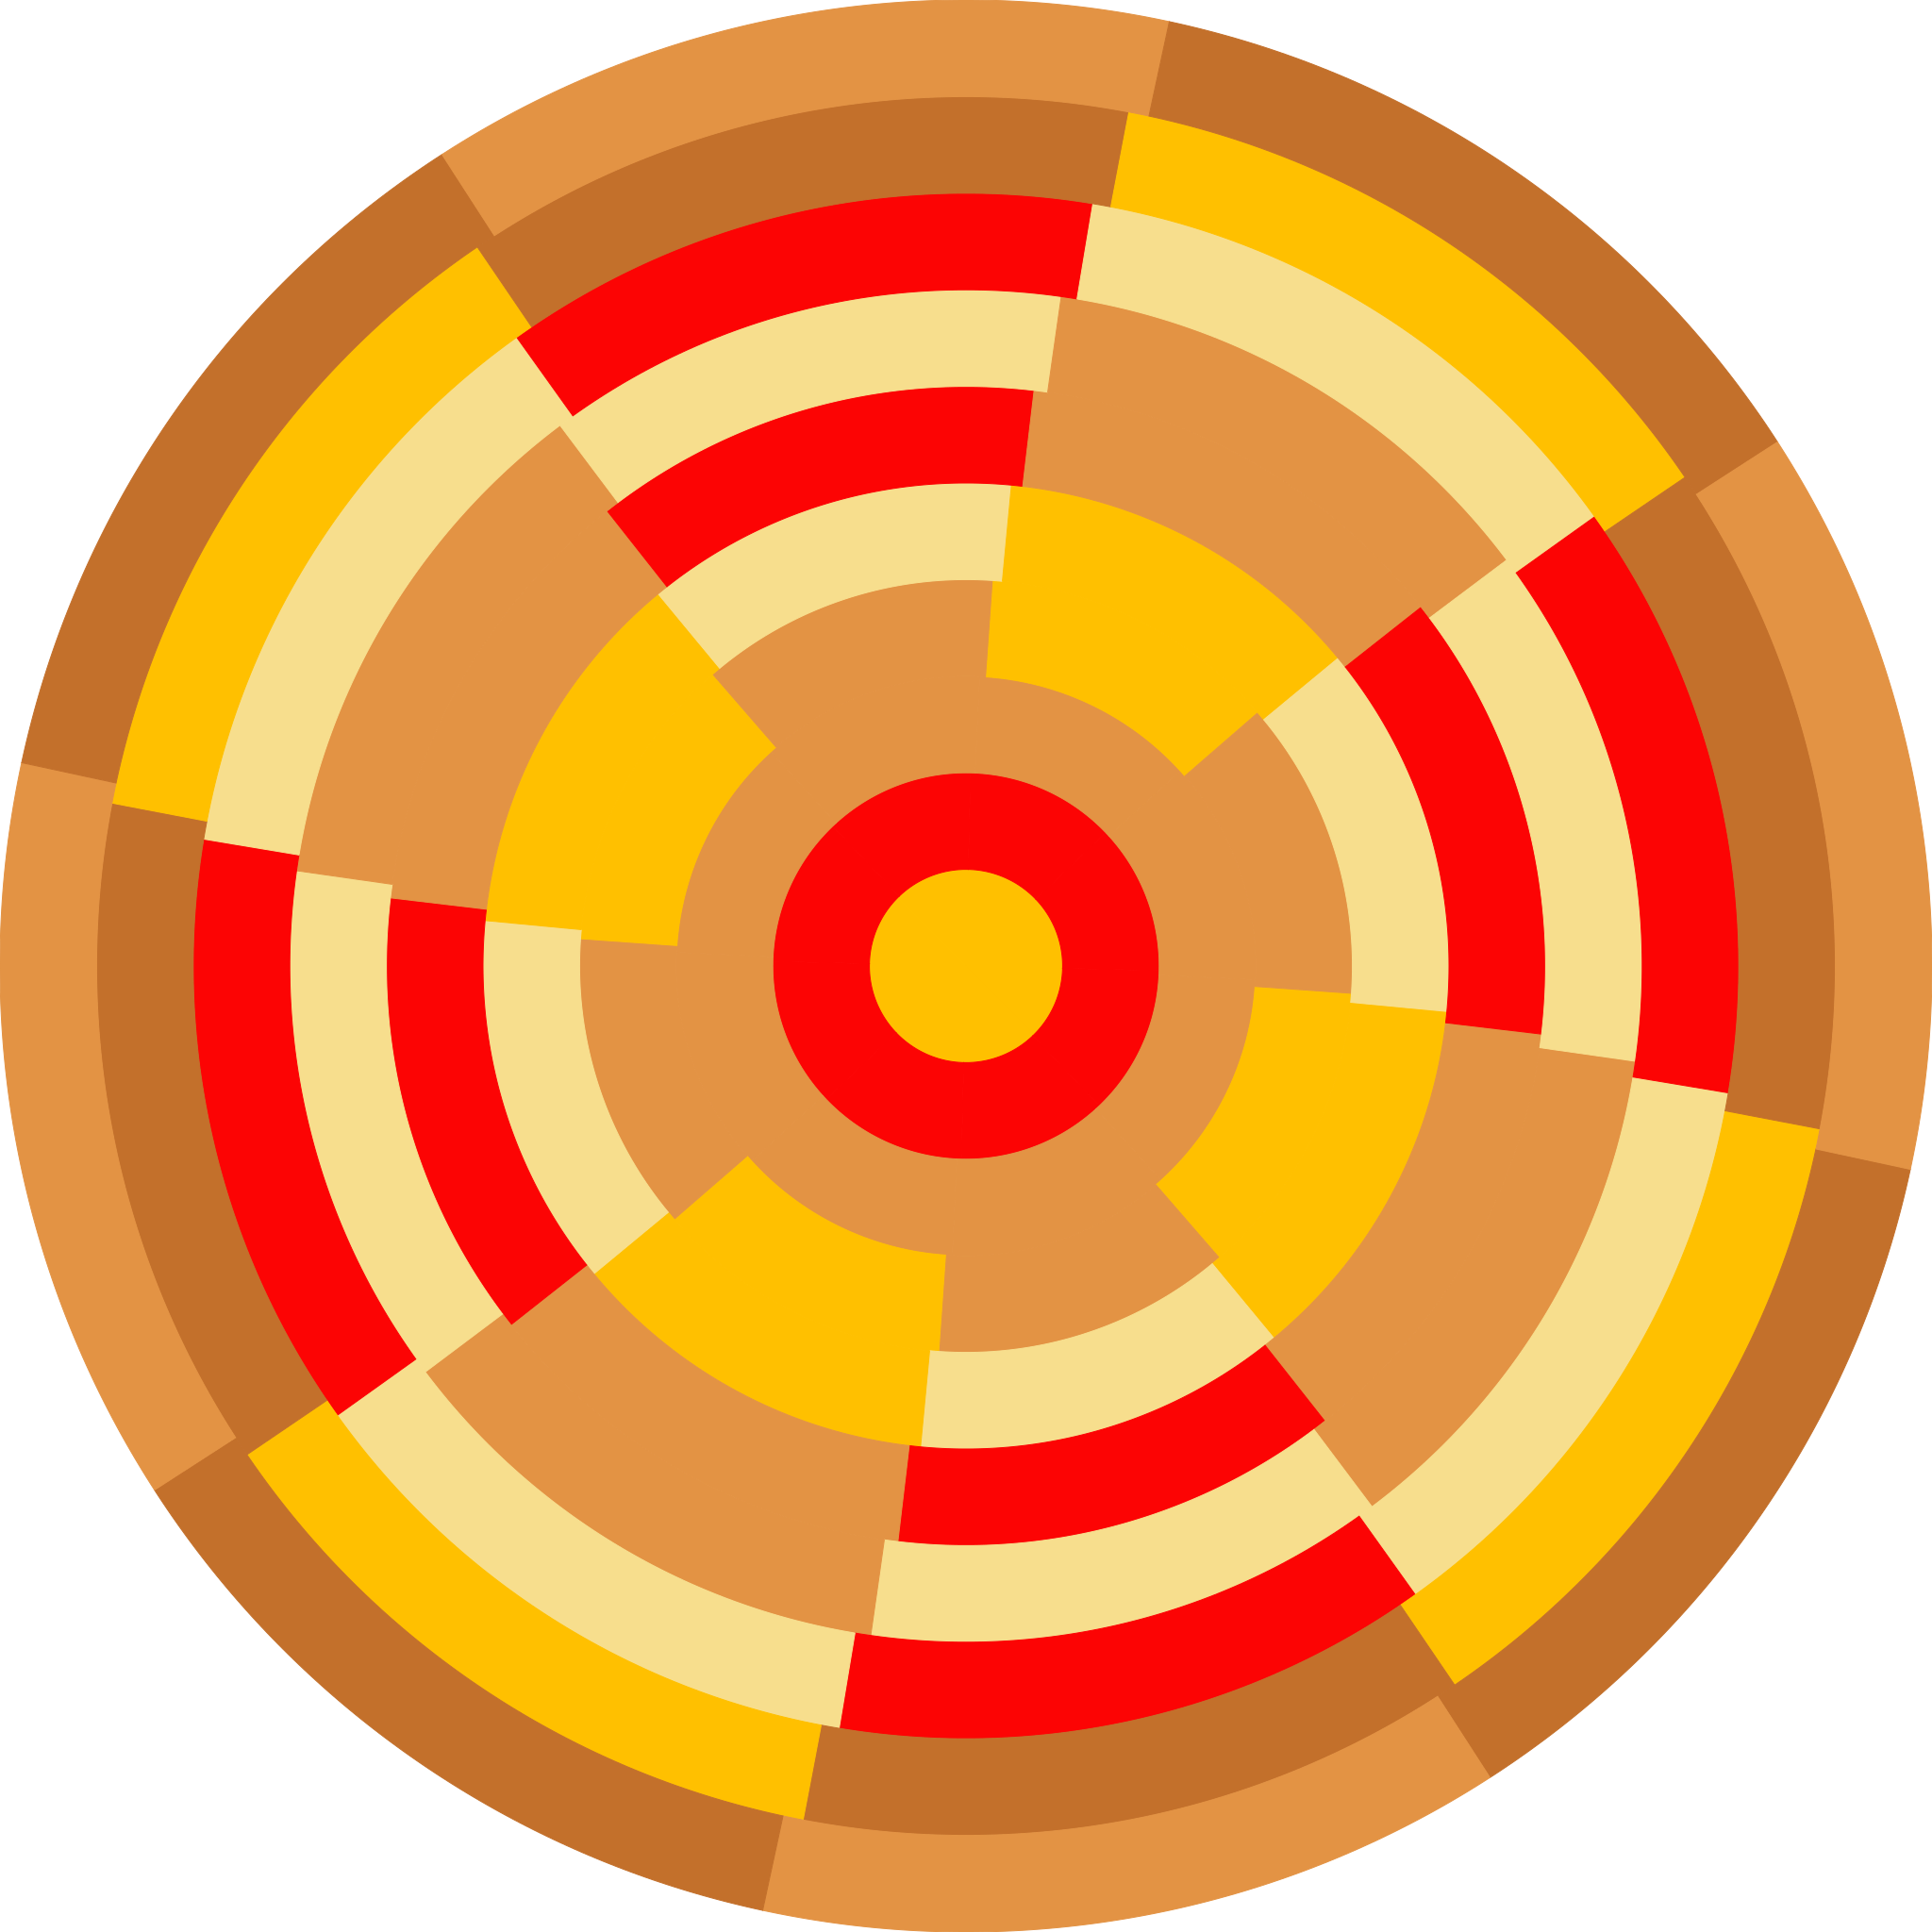
\includegraphics[width=0.3\textwidth]{images/reduction/10/disc.png}
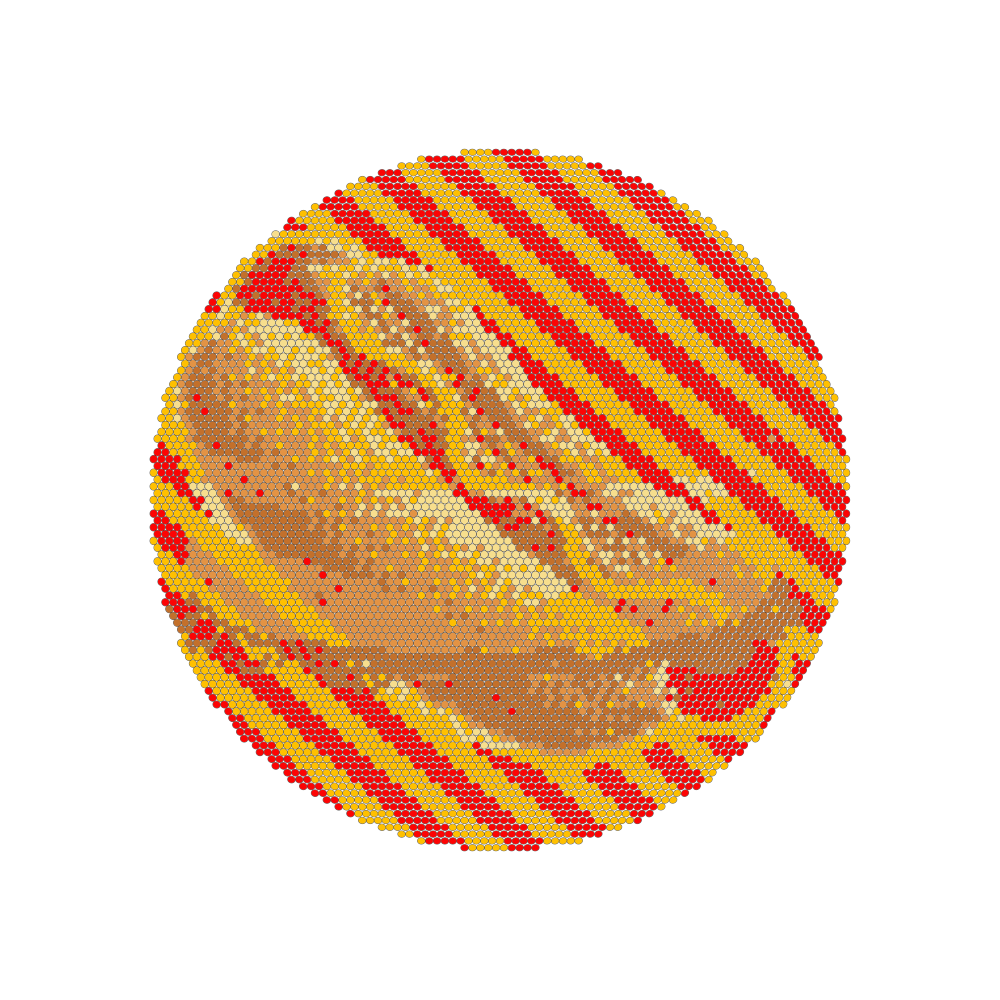
\includegraphics[width=0.3\textwidth]{images/reduction/10/sim0.png}
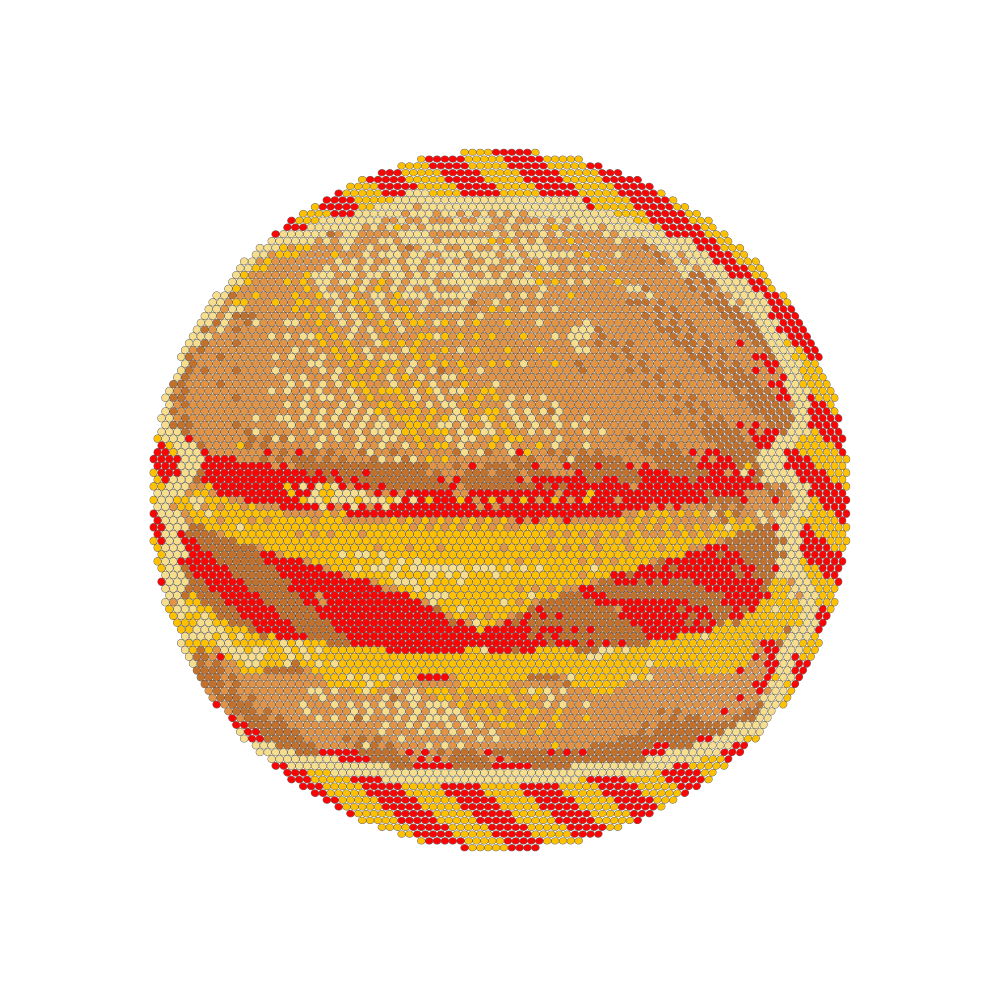
\includegraphics[width=0.3\textwidth]{images/reduction/10/sim1.png}
\caption{10 sequences}
\end{subfigure}

%\end{figure}
%\begin{figure}[ht!]
%\ContinuedFloat

\begin{subfigure}[t]{0.4\textwidth}
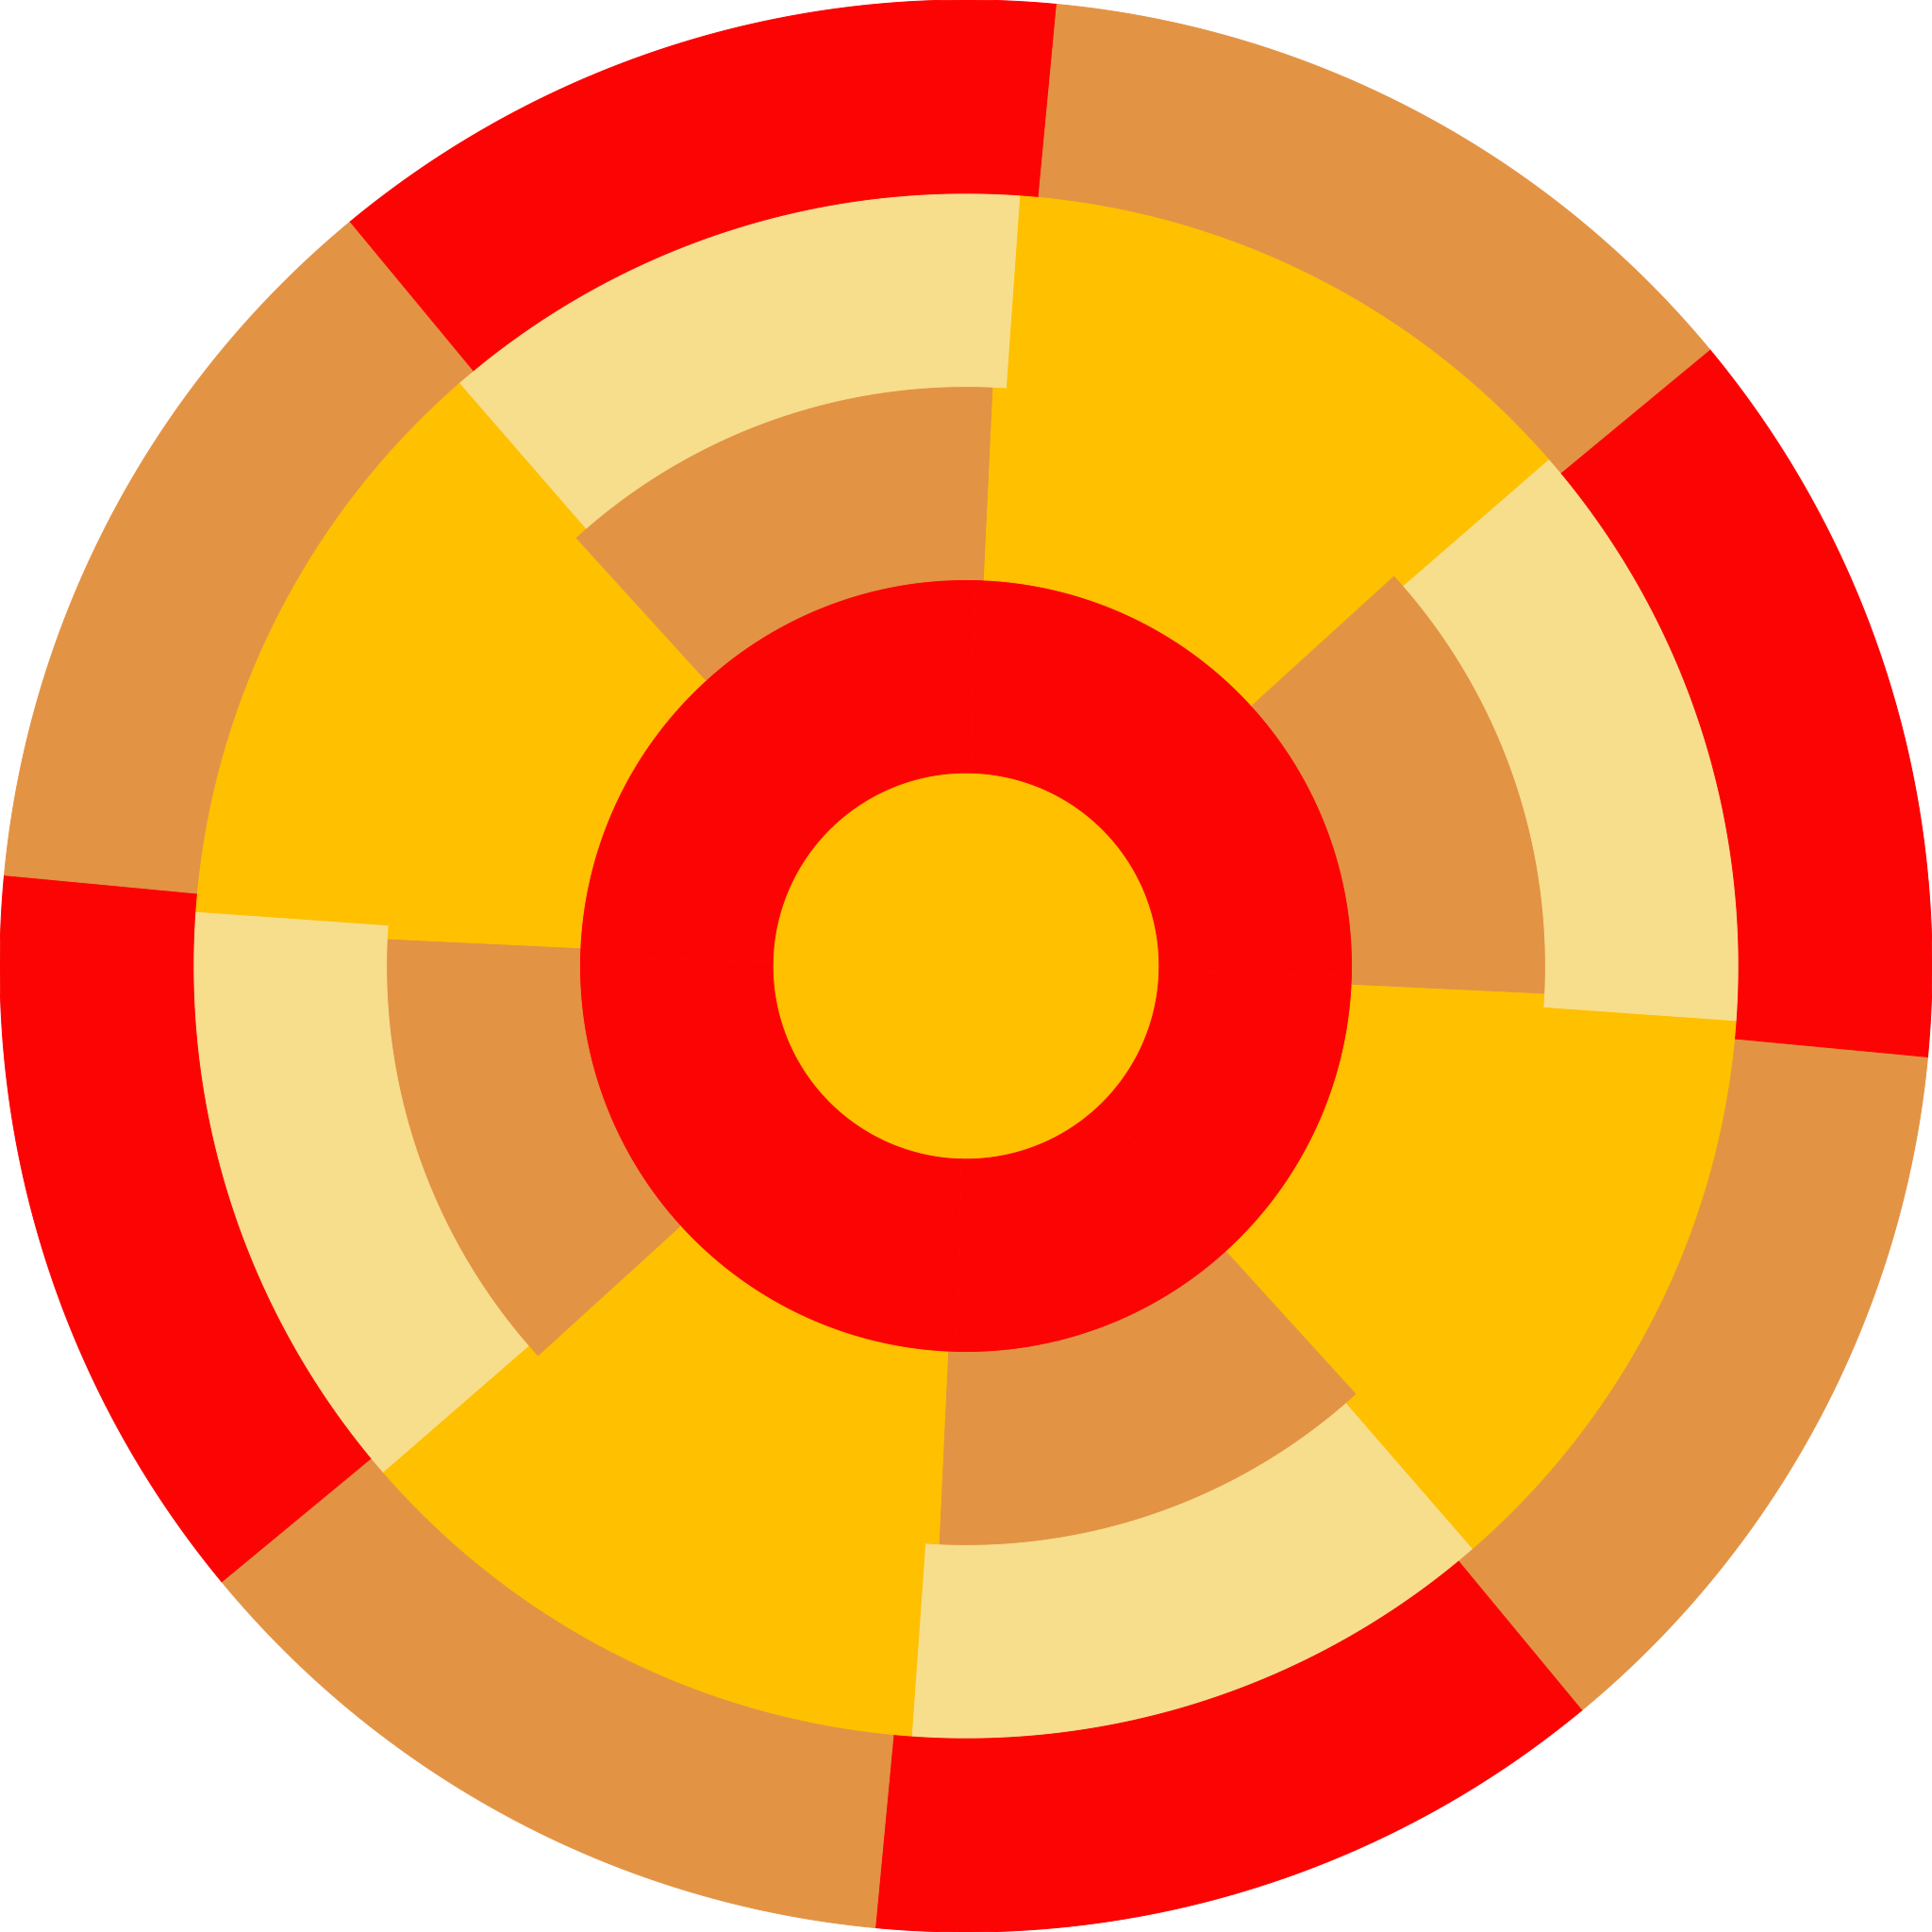
\includegraphics[width=0.3\textwidth]{images/reduction/5/disc.png}
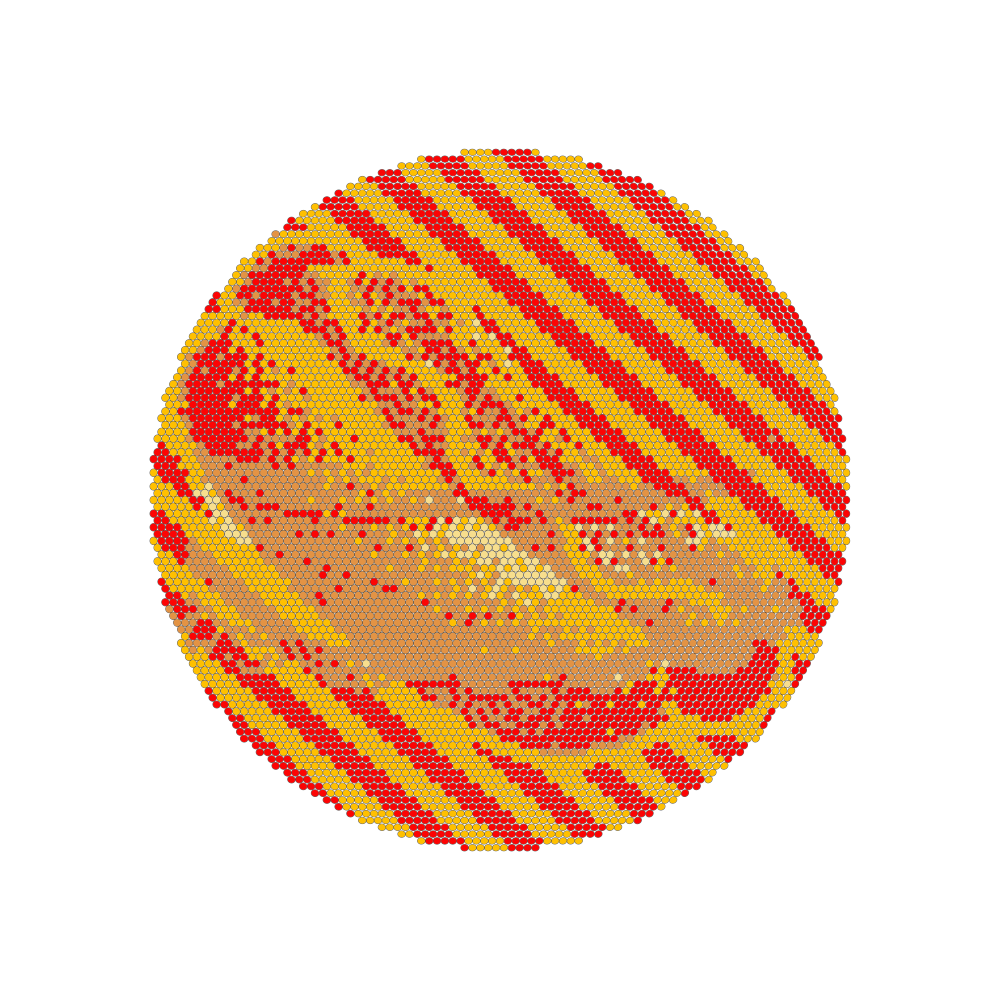
\includegraphics[width=0.3\textwidth]{images/reduction/5/sim0.png}
\includegraphics[width=0.3\textwidth]{images/reduction/5/sim1.png}
\caption{5 sequences}
\end{subfigure}
\hfill
\begin{subfigure}[t]{0.4\textwidth}
\includegraphics[width=0.3\textwidth]{images/reduction/1/disc.png}
\includegraphics[width=0.3\textwidth]{images/reduction/1/sim0.png}
\includegraphics[width=0.3\textwidth]{images/reduction/1/sim1.png}
\caption{1 sequence}
\end{subfigure}

\caption{ The first row shows the animation with 35 sequences. The palette disc is really struggling to fit all sequences but the resulting images are vivid with colors and contrast. After reducing to 30 sequences not much can be seen visually but it's possible to see some brown spots in the red line to the left of the hotdog from a strong reduction in sequences containing green. By 25 sequences all green color has been removed and the hamburger image bleeds into the hotdog. The reduction to 20 sequences doesn't change much but the hamburgers tomato and right side of the bun is starting to leak into adjacent areas. At 15 sequences all darker colors have disappeared and we are starting to loose contrast. The sausage also see significant ghosting from the hotdog. At 10 we are down to five colors from the original eight. The meat in the burger are clearly ghosting. At five sequences its still possible to guess the original images but it's getting hard. Finally at one sequence there is just a mess of brown left and where the first image is the inverse of the second.}
\label{fig:reducing}
\end{figure}



\section{Using Software to simulate the mirror setups for rapid iterations.}

To be able to verify that all the calculation has been made right it is
very helpful to first run a simulation \emph{in silico}\footnote{\emph{In
  silico} refers to doing something on the silicon i.e. on a computer
  (computer chips are made out of silicon). It is a term is pseudo-latin
  (the correct term would have been in \emph{silicio}) and alludes to
  the latin terms \emph{in vivo} (for experiments on living biological
  organisms in their habitat), \emph{in vitro} (for experiments on
  organisms in test tubes) and \emph{in situ} for experiments taken
  place on site.}. This enables rapid iterations and verification.
Building the mirrors and testing it out just to realize some
calculations was wrong would be very costly.

My pipeline consists of a custom software that takes as input a
\texttt{.png} or \texttt{.jpeg} image. Then it converts the pixel
position from a rectilinear coordinate system to a hexagonal using sub
pixel sampling. Then the software assembles the palette. If that initial
palette contains too many colors it is reduced using the methods
described above. When the palette colors are computed it creates a
color field texture and exports it as a \texttt{.png} image as well as
the coordinates for the color field centers. Further it computes the
angles of all the mirrors given the position, size and orientation of
the color fields, the mirror and the spectator. Then the software
creates a \texttt{.obj} file with a 3d model of all mirrors and color
fields and some additional debug information. That 3d model can be
imported into any 3d-rendering software (I use Blender) for light
simulation. Blender is able to simulate the light rays emitted from a
lamp and how they reflect on the color fields and on the mirrors and
then end up in a virtual camera.

\begin{figure}[ht!]
\centering
\includegraphics[width=0.8\textwidth]{images/simulation/rooster.png}
\caption{Rendering Leonardo with light ray path tracing.}
\end{figure}

Having a 3d-model that can be rendered with in a plausible physics
simulation makes it a lot easier to see what happens when there are any
misalignments.

If one also wants to simulate caustics and volumetric materials I can
highly recommend installing the LuxCore plugin for Blender that uses
the Bidir rendering engine. See the \emph{Calibration} section for
details and figures.


\section{Fabricating the mirror array panel}

While calculating the angles and positions of the mirrors in an
idealized world is one thing, actually reproducing the same with high
accuracy and precision\footnote{Accuracy is how close to a given set of
  measurements are to their true value while precision is how close or
  dispersed the measurements are to each other. BS ISO 5725-1, 1994,
  \emph{Accuracy (trueness and precision) of measurement methods and
  results - Part 1: General principles and definitions.}}. A small angle
of error of the mirrors might multiply quickly over relatively long
distances and make the mirror reflect a different position than was
calculated for. It is therefore of paramount importance that,
especially, the angles of the mirrors can be positioned as
calculated.

I have experimented with a few different techniques that I intend to
describe in this chapter.


\subsection{3D-printing}

The most common 3D-printer technology is called FDM\footnote{Fused
  Deposition Modeling} and works by placing a string of melted plastic
layer by layer until the entire desired volume is filled. Usually each
layer is about 0.25 mm thick which is enough to be noticeable both
by looking at the finished part and by touch. Since the layers are
relatively thick and each layer has the same thickness it can be hard to
produce surfaces with very shallow slopes which is exactly what we want
to do. For example a slope with 1$^{\circ}$ incline only changes the height of 0.174 mm over 10 mm that would result in a reflection target change of about 17 mm at a mirror-to-color-field distance of 1m. This means that it is physically impossible to print that on a regular FDM printer (since the minimum layer height is 0.25 mm, more than double the required height).


\begin{figure}[ht!]
\centering
\includegraphics{images/layer-lines-25mm.png}
\caption{3D-printing with a surface with a slope of 1° using layer height of 0.25mm results in the layers being too thick (black line). The desired surface (red, dashed) would intersect one of the layers and also not being supported anywhere else.}
\end{figure}

Another type of 3D-printer is the SLA \footnote{Stereolithography
  Apparatus, also called Photosolidification printers or more commonly
  Resin printers.} printers. They work by selectively cure a
photosensitive resin layer by layer with an UV-projector. The same problems apply as with FDM
but it is possible to achieve much higher resolutions (up to 0.01 mm).
Even with this very high resolution it is still only about two layer
steps over 10 mm supporting a 1° sloping surface.

\begin{figure}[ht!]
\centering
\includegraphics{images/layer-lines-01mm.png}
\caption{3D-printing with a surface with a slope of 1° using layer height of 0.1mm (black line) results in the desired surface (red, dashed) would not be supported on anything but two points. The resolution is too low to have multiple steps support the surface. To achieve good results the layer needs to be much thinner to be able to closely approximate the desired surface slope.}
\end{figure}


My testing confirms the thesis that it's difficult to produce substrates
that a mirror can be glued to with high enough precision and accuracy
using FDM and SLA printers.


\subsection{Milling}

The second option to create a surface for gluing mirrors is
CNC\footnote{Computer Numerical Control}-milling the surface. Milling
does the opposite of 3D-printing by, instead of adding, removing
material. It is using something that looks like a drill but that is
ground sharp not only at the tip but also at the sides to carve away
material both axially and radially. I'm not going to go into depth on how a milling machine works
but you can think of it as a rod that spins very rapidly and everything
it touches becomes dust.

Here we can also reap the benefits of using a round mirror that we talked about in the section about arranging the mirrors. 
Since the milling bit tool is round it cannot create holes with sharp inside corners but it can with ease create round holes.
This means that we can, without effort, create holes that the mirrors will fir snugly in. 

The most common type of milling machines are called 3-axis machines. As
the name suggests the tool can move in three axes. The standard
nomenclature is calling the left/right axis \emph{X}, the towards/away
axis \emph{Y} and the up/down axis \emph{Z}. Since the tool is always
aligned to the Z-axis it can not produce overhangs\footnote{This is
  technically not correct since it is possible to have a variable-radius
  tool with a thinner shank that reach in under an overhang.}. It's
usually said that a 3-axis machine can only mill 2.5 dimensions models
since it cannot machine on all sides of the object, only those reachable
straight from the top . This also means that the tip of the tool can not
be aligned perpendicular to the surface that we want to machine (as it
is always aligned to the Z-axis) we are still confined to milling steps
of some sort. This can of course be partially alleviated by milling in
the direction of the slope, continually adjusting all axes
simultaneously, but the geometry of the cutting tool will still either
produce grooves or we will have to cut with an an infinitely small tool.

\begin{figure}[ht!]
\centering
\includegraphics{images/milling-z-aligned.png}
\caption{A 3-axis milling machine always aligns the tool with the Z-axis. This results, just as the 3D-printing, in steps. Even though a CNC-milling machine can achieve higher resolution it is still going to produce steps.}
\end{figure}

In my experiments using a 3-axis CNC can produce working parts but is
not able to create perfect sockets for the mirrors to sit in (since
that would require machining overhangs). To achieve high enough
resolution one have to take very small step-overs and machine the same
surface multiple times in multiple directions which leads to very long
machining times. One experiment I did was 630x480 mm and took over nine
continuous hours to machine.

To achieve full 3 dimensional models one have to use a 5-axis mill. The
two extra axes called roll and pitch (and usually denoted the B- and
C-axis) allows the tool to align to the surface normal of the model.
This means that making a very accurate round socket for the mirror is as
easy as aligning a properly sized tool in the desired angle and then
just plunging into the stock material. This makes this method very fast
in comparison since it is basically only machining the geometry we want
and nothing else. Professional machines can hold tolerances within one
arc-second\footnote{One arc-second equals 1/3600 \textsuperscript{th} of
  a degree.} which is plenty accurate for what our application and many
orders of magnitude more than what can be done with previously mentioned
techniques.

\begin{figure}[ht!]
\centering
\includegraphics{images/milling-tool-aligned.png}
\caption{A 5-axis milling machine can aligned the tool to the desired surface normal (red-dashed) and can therefore plunge into the material creating a pocket with the desired angle.}
\end{figure}


When milling we also have the benefit over other techniques that 
we can work in basically any material. One consideration that has to be taken into account
when selecting material is warping. If there are stresses in the material
from for example painting the surface it has a tendency to bend away
from the surface being machined when the one side is partially removed.
This is true for most materials both organic, like wood, and inorganic, like metals and plastics.

I have mainly used dyed through HDF\footnote{High Density Fiberboard}
since it relatively cheap, slightly harder than MDF\footnote{Medium Density Fiberboard} and therefore
retains a sharp edge better, has mixed directional fibers making it
less prone to warping and is less effected by temperature and humidity
changes than for example wood. I have also done some experiments with
perspex boards that showed good results but had a tendency of producing
a burr that had to be manually removed and is also quite a bit more
expensive.

If one has access to a 5-axis milling machine I highly recommend using
one. When the pockets have been milled the mirrors can be glued into the
pockets. Since the pockets are perfectly flat bottomed and the sides of
the pockets are normal to the bottom surface the mirror is very easy to
align. I'm using super glue holds the mirrors firmly and dries fast. It
might be possible to use other types of glue but I haven't tested that.

\begin{figure}[ht!]
  \centering
  \begin{subfigure}[t]{0.45\textwidth}
    \includegraphics[width=0.8\textwidth]{images/milling.jpeg}
    \caption{Using a 5-axis milling machine to create angled pockets for mirrors in a black HDF.}
  \end{subfigure}
  \hfill
  \begin{subfigure}[t]{0.45\textwidth}
    \centering
    \includegraphics[width=0.8\textwidth]{images/mirror_pockets.png}
    \caption{10mm mirrors being glued into the angled pockets of a HDF board.}
  \end{subfigure}
\end{figure}


\section{Calibrating}

Collectively the mirrors act like a lens and hence has a focal plane
(rather than a focal point that some lenses have). The objective of
calibration is to position the color fields aligned along the focal
plane and at the correct position within that focal plane. If you
imagine a four by four, square color field and the targets of the
mirrors are in the center of each separate color field one can imagine
that there will be multiple focal points where light rays from multiple
mirrors converge. All those focal points will lie on the focal plane. 
If the color field is outside the focal plane there
will be no convergence and some rays may miss the target field leaking
into other color fields.

As we already have established optics are geometrically reversible. This
opens for a simple way to visualize the light path to be able to
accurately position the mirrors, spectator and color palette in
relation to each other. By placing a strong point light source at the
position of the spectator shining on the mirrors a pattern of lit dots
will appear on the color fields. This way one can visually inspect
exactly where the targets will be with the current positioning and it's
easy to make small adjustments to fix any errors by either moving the
color fields, the mirrors or the spectator. This can be done both in
silico as well as in situ.

\begin{figure}[ht!]
\centering
\includegraphics[width=1.0\textwidth]{images/simulation/calibration.png}
\caption{Simulation with a light beam striking the mirrors in a smokey room to visualize the light paths. From the left, the first image depicts a correct calibration where all the focal points are positioned in the center of each color field. The second image shows the color field moved in front of the focal plane. The third image shows what happens when the color fields are positioned behind the focal plane making the rays converge and then diverge before it hits the color fields. It best shown in the upper left corner where it is easy to see the focal point laying in front of the color fields.}
\end{figure}


\begin{figure}[ht!]
\centering
\includegraphics[width=0.6\textwidth]{images/calibration-photo.png}
\caption{Ongoing calibration in the field. It looks very similar to the simulated version.}
\end{figure}


Moving the position of the spectator could also have a very large
effect. This of course depends on the relation of the distances between
the spectator and the mirrors and the mirrors and the color fields. If
the distance between the spectator and mirror is larger than the mirror
and color fields distance the spectator can move more without the
targets on the color field moving. It basically acts as an optical
lever.


% \begin{figure}[ht!]
% \centering
% \begin{frame}{Embedded Animation}
%   \animategraphics[loop,controls,width=\linewidth]{10}{images/simulation/animation/}{1}{20}
% \end{frame}
% \caption{Simulated animation of the effect of the coulour field targets as the spectator moves in relation to the mirrors.}
% \end{figure}

\clearpage

\section{Results}

So far I have fabricated five images using the techniques described in
this paper. I'm here going to present them in chronological order of
fabrication.

\subsection{Nightshades}

The \emph{Nightshades} was the first image I made. At this point, the most
interesting was to figure out if this would actually work in reality. I
struggled for a very long time trying to figure out what images to use.
After months of experimenting with different images and having a hard
time deciding on one someone said "It's tomato/tomato" so I figured a
tomato and a potato would work (both flowering plants of the
\emph{Solanaceae} or the \emph{Nightshades} botanical family). The
sculpture is set up so that first a tomato is displayed and as the
disc slowly rotates it will quickly switch over to a potato and then
repeating the animation. Technically the trickiest thing was to reduce
the palette enough to fit the resulting disc and while keeping enough
colors to be able to see both images. I've used dithering shading on
both images to create more perceived colors than actually exist. The
light brown color used for the highlight of the potato is also
red-tinted enough to be used as highlight of the tomato. The tomatoes
green leafs are actually made up of the green background plus a brown
dithering pattern to make it look a dark green. I've also slightly
edited the image to remove some color sequences. For example the
highlight on the tomato has a missing section to avoid a
light-brown/light-brown sequence that would also be used for those
10-ish mirrors.

Something to note is that diagonal dithering does not translate well
when mapping the mirror pattern from rectilinear to hexagonal. There is
a tendency to create streaks of colors when converting to hexagonal if
the coordinate systems are mapped directly. I have since transitioned
to using the sub-pixel sampling method instead.

\begin{figure}[ht!]
\centering
\includegraphics[width=0.3\textwidth]{images/potato-tomato/input_1.png}\includegraphics[width=0.3\textwidth]{images/potato-tomato/input_0.png}\includegraphics[width=0.3\textwidth]{images/potato-tomato/disc.png}
\caption{Input images and color field texture}
\end{figure}

\begin{figure}[ht!]
\centering
\includegraphics[width=0.4\textwidth]{images/results/potato_tomato_1.jpg}
\includegraphics[width=0.4\textwidth]{images/results/potato_tomato_2.jpg}
\caption{Built structure}
\end{figure}

\pagebreak

\subsection{We know how to live}

\emph{We know how to live} is the title of a song on \emph{Cock
Sparrer's} 1994 album \emph{Guilty as charged}. In the song they sing
"Mugs of tea, the sun and lager - we know how to live". I found it quite
amusing that the song, being a punk rock/oi song, was celebrating
something mundane as mugs of tea. To avoid getting stuck picking images
I figured I'd just have commit quickly before I'd change my mind or
start doubting the idea.

The texture is wrapped around a rotating cylinder so that at least three
columns are visible to the mirrors at all times. Since all objects in
the picture is set on a solid white background and none of them overlap
I can exploit the fact that the resulting texture will contain as many
sequences as there are unique colors. 

\begin{figure}[ht!]

\centering
\includegraphics[width=0.25\textwidth]{images/tea-sun-lager/input_0.png}\includegraphics[width=0.25\textwidth]{images/tea-sun-lager/input_1.png}\includegraphics[width=0.25\textwidth]{images/tea-sun-lager/input_2.png}\includegraphics[width=0.25\textwidth]{images/tea-sun-lager/texture.png}
\caption{Input images and color field texture}
\end{figure}

\begin{figure}[ht!]
\centering
\includegraphics[width=0.3\textwidth]{images/results/we_know_how_to_live_2.jpg}\includegraphics[width=0.3\textwidth]{images/results/we_know_how_to_live_1.jpg}\includegraphics[width=0.3\textwidth]{images/results/we_know_how_to_live_3.jpg}
\caption{Built structure}
\end{figure}

\pagebreak

\subsection{Leonardo}

\emph{Leonardo} was the name of a rooster I bought from a friend for
five SEK while at kindergarten. The name Leonardo referred to the
\emph{Teenage Mutant Ninja Turtle} "Leonardo"\footnote{Leonardo was the
  Ninja Turtle wearing a blue bandana and had double Ninjatos as his
  signature weapon (commonly confused as Katanas). Of course the Ninja
  Turtles name Leonardo in turn refers to the renaissance painter and
  inventor Leonardo da Vinci. The other Ninja Turtles was called
  \emph{Rafael} (red, twin sai), \emph{Michelangelo} (orange, dual
  nunchaku) and \emph{Donatello} (purple, bō staff).} that was all the
rage in the late 80's and early 90's. After having made
\emph{Nightshades} and \emph{We know how to live} I thought it was a
little bit too difficult as a spectator to find the optimal position
since the color fields were relatively small. I wanted to do something
that had some more colors and I was a little disappointed that it was
possible to discern the mug, sun and beer glass in \emph{We know how to
live} without having the color palette present. I scrolled through
emojis trying to find something colorful and decided on the rooster. I
tried to dither it quite hard and also added a gradient background to
add noise to the image. From this came a palette of 16 colors. Four
shades of pink, four of red, four of brown and four of blue. I sorted
the colors by darkness and painted it on textile patches that I sewed
together into a 3.5x3.0m large curtain.


\begin{figure}[ht!]
\centering
  \begin{subfigure}[t]{0.45\textwidth}
    \centering
    \includegraphics[width=0.5\textwidth]{images/rooster/input_0.png}\includegraphics[width=0.5\textwidth]{images/rooster/texture.png}
    \caption{Input image and color field texture}
  \end{subfigure}
  \begin{subfigure}[t]{0.45\textwidth}
    \centering
    \includegraphics[width=0.9\textwidth]{images/results/leonardo.jpg}
    \caption{Built structure}
  \end{subfigure}
\end{figure}

\pagebreak

\subsection{Brontide}

I realized after making the big textile used for \emph{Leonardo} that I
could reuse it to show other images. The only problem was that the
color palette was already set and it was not the most usable. Had I
anticipated this I had maybe added some more base colors like green,
orange or purple. But I had what I had so I started to look for images
that could work with that palette. I had watched a documentary of
volcanoes squirting magma into the sea that I thought could fit. I also
liked the idea of the very noisy and chaotic image since that would make
it even more difficult to see what was depicted without the color
fields. After googling around for volcanoes a couple of days I found a
still from the 1940 Disney animated musical \emph{Fantasia} with a very
nice erupting volcano and also containing mostly bluish and reddish
tones.

\emph{Brontide} is a word for the low, muffled sound of thunder at a
distance or the sound of seismic activity\footnote{The name of the long
  necked dinosaur \emph{Brontosaur} has the same etymology stemming from
  \emph{"bronte"} being greek for \emph{"thunder"} and \emph{"souros"}
  meaning \emph{"lizard"}. The suffix \emph{-id} means "offspring of" or
  "coming from" so \emph{Brontide} is something that comes from thunder.}.

\begin{figure}[ht!]
\centering
  \begin{subfigure}[t]{0.45\textwidth}
    \centering
    \includegraphics[width=0.5\textwidth]{images/volcano/input_0.png}\includegraphics[width=0.5\textwidth]{images/volcano/texture.png}
    \caption{Input image and color field texture}
  \end{subfigure}
  \begin{subfigure}[t]{0.45\textwidth}
    \centering
    \includegraphics[width=0.9\textwidth]{images/results/brontide.jpg}
    \caption{Built structure}
  \end{subfigure}
\end{figure}

\pagebreak

\subsection{Strokes}

The last in the textile palette series is \emph{Strokes}. I thought it
would be interesting to do something abstract where the "correct"
position doesn't matter that much. I used Photoshop but couldn't really
make anything that I thought worked so I just made a lot of strokes like
you would when striking out a misspelled word. I kept on adding more
lines in different colors and there it was like colorful pick-up
sticks.


\begin{figure}[ht!]
\centering
  \begin{subfigure}[t]{0.45\textwidth}
    \centering
    \includegraphics[width=0.5\textwidth]{images/lines/input_0.png}\scalebox{-1}[1]{\includegraphics[width=0.5\textwidth]{images/lines/texture.png}}
    \caption{Input image and color field texture}
  \end{subfigure}
  \begin{subfigure}[t]{0.45\textwidth}
    \centering
    \includegraphics[width=0.9\textwidth]{images/results/strokes.jpg}
    \caption{Built structure}
  \end{subfigure}
\end{figure}

\end{document}
